\section{Vista de escenarios}
La siguiente Figura \ref{fig:CU_General} \nameref{fig:CU_General} muestra  el diagrama de los casos de uso de la herramienta, contemplando a dos actores finales: Entrenador y Practicante.\\

\begin{figure}[H]
	\begin{center}
		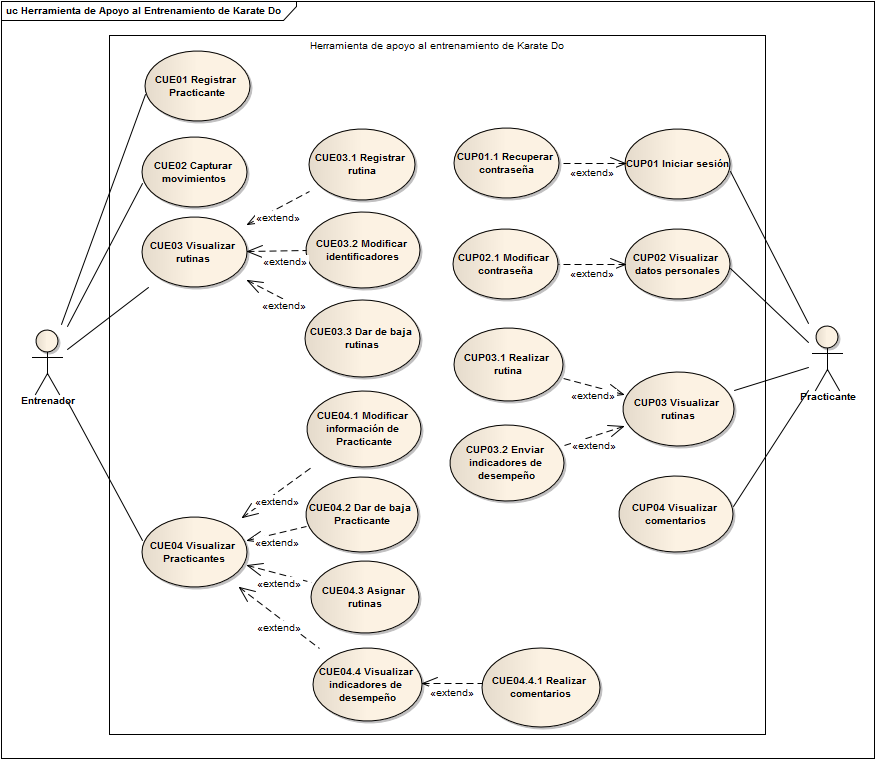
\includegraphics[scale=0.5]{./Figuras/Casos/CUGeneral}
	\end{center}
	\caption{Casos de uso Herramienta de apoyo al entrenamiento de Karate-Do}
	\label{fig:CU_General}
\end{figure}

\clearpage
%------------------------------------------------------------------------------------
\subsection{Casos de uso aplicación Entrenador}
La Figura \ref{fig:CU_Entrenador} \nameref{fig:CU_Entrenador} que se presenta a continuación, muestra el diagrama de los casos de uso correspondientes al actor Entrenador, además seguido de este se muestran las descripciones y trayectorias de cada uno de ellos.

\begin{figure}[H]
	\begin{center}
		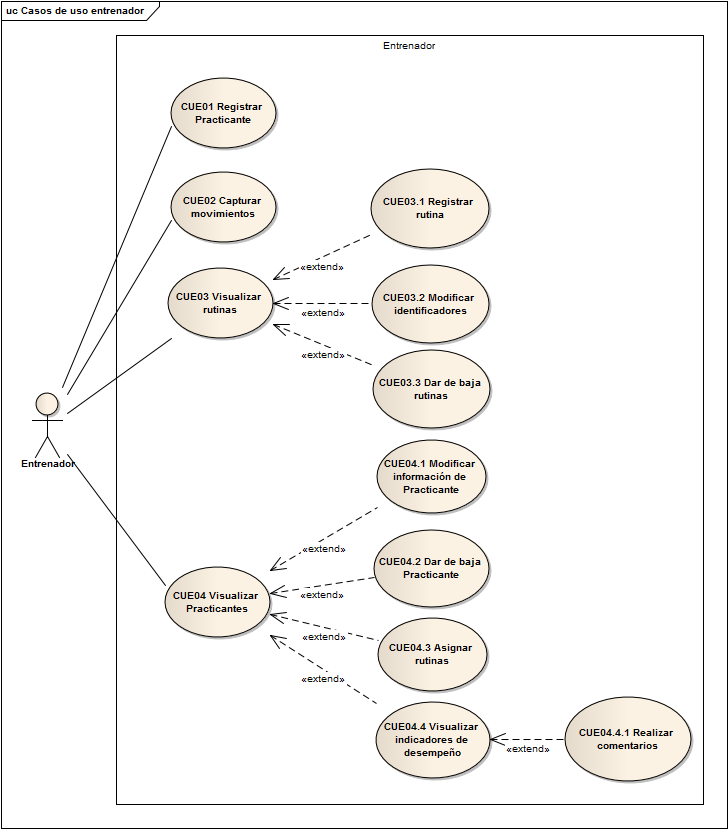
\includegraphics[scale=0.6]{./Figuras/Casos/Casos_de_uso_entrenador}
	\end{center}
	\caption{Casos de uso - Entrenador}
	\label{fig:CU_Entrenador}
\end{figure}

\subsubsection{CUE01 Registrar Practicante}
\label{cu:CUE01}
%--------------------------------------------------------------------------------------------------------
\textbf{\textcolor[rgb]{0, 0, 0.545098}{Resumen}} \\

Este caso de uso brinda al Entrenador la posibilidad de generar el registro de un Practicante, facilitando al Entrenador contar con un control de los Practicantes registrados en la herramienta así como de los datos relevantes de cada uno de ellos, de los cuales realiza el seguimiento de su desempeño.\\

\textbf{\textcolor[rgb]{0, 0, 0.545098}{Descripción}} \\

\begin{table}[H]
\centering
\begin{tabular}{| l | p{12 cm} |}
\hline
\rowcolor[rgb]{0.529412, 0.807843, 0.980392} {\textbf{Caso de uso:}} & \hspace{7em}{\textbf{CUE01 Registrar Practicante}}\\
\hline
\textbf{Actor:} &  \nameref{act:Entrenador}. \\
\hline
\textbf{Objetivo:} & Permitir al Entrenador registrar un nuevo Practicante.\\
\hline
\textbf{Entradas:} & Para llevar a cabo el registro de un nuevo Practicante, el Entrenador deberá hacer uso de la pantalla \nameref{pant:IUE01} y deberá capturar la siguiente información:
		\begin{compactitem} 
			\setlength\itemsep{-0.25em}
			\item Nombre(s)del usuario. Se escriben desde el teclado.
			\item Apellido(s). Se escriben desde el teclado.
			\item Edad. Se escribe desde el teclado.
			\item Domicilio. Se escribe desde el teclado.
			\item Teléfono. Se escribe desde el teclado.
			\item Correo electrónico. Se escribe desde el teclado.
			\item Avatar del Practicante. Se selecciona con el mouse.
			\item Peso. Se escribe desde el teclado.
			\item Estatura. Se escribe desde el teclado.
			\item Grupo sanguíneo. Se selecciona con el mouse.
			\item Grado de cinta. Se selecciona con el mouse.
			\item Nombre de usuario. Se escribe desde el teclado.
		\end{compactitem} \\
\hline
\textbf{Salidas:} & \vspace{-2mm}	%Para quitar el espacio en blanco de la fila
					\begin{compactitem}
						\setlength\itemsep{-0.25em}
						\item Se muestra en la pantalla \nameref{pant:IUE01}, el mensaje \nameref{msj:MSG01}, cuando se registre un Practicante de manera exitosa.
						\item Se envía al correo electrónico registrado el mensaje de tipo correo \nameref{msj:MSG08}, enviando la información de usuario y contraseña correspondiente.
					\end{compactitem}\\
\hline
\textbf{Precondiciones:} & \vspace{-2mm}	%Para quitar el espacio en blanco de la fila
							\begin{compactitem}
								\setlength\itemsep{-0.25em}
								\item El Practicante no debe estar registrado previamente en la herramienta.
							\end{compactitem}\\
\hline
\textbf{Postcondiciones:} & \vspace{-2mm}	%Para quitar el espacio en blanco de la fila
							\begin{compactitem}
								%\setlength\itemsep{-0.25em}
								\item Se registrará en la herramienta un nuevo Practicante.
								\item Se actualizará el catálogo: \textit{Practicantes}
							\end{compactitem}\\
\hline
\end{tabular}
\end{table} 

\begin{table}[H]
\centering
\begin{tabular}{| c | p{12 cm} |}
\hline
\textbf{Reglas de negocio:} & \vspace{-2mm}	%Para quitar el espacio en blanco de la fila
							\begin{compactitem}
								%\setlength\itemsep{-0.25em}
								\item \nameref{rn:RNR01}.
								\item \nameref{rn:RNR02}.
								\item \nameref{rn:RNR03}.
								\item \nameref{rn:RNR04}.
								\item \nameref{rn:RNR05}.
								\item \nameref{rn:RNR06}.
								\item \nameref{rn:RNR07}.
								\item \nameref{rn:RNR08}.
								\item \nameref{rn:RNR10}.
								\item \nameref{rn:RNR11}.
								\item \nameref{rn:RNR13}.
							\end{compactitem}\\		
\hline

\textbf{Errores:} & \vspace{-2mm}	%Para quitar el espacio en blanco de la fila
					\begin{compactitem}
						\setlength\itemsep{-0.25em}
						\item Se muestra en la pantalla \nameref{pant:IUE01} el mensaje de error \nameref{msj:MSG12} cuando el Entrenador no haya ingresado datos a los campos obligatorios.
						\item Se muestra en pantalla el mensaje de error \nameref{msj:MSG13} cuando el Entrenador haya ingresado datos con un formato incorrecto en algún campo.
						\item Se muestra en pantalla el mensaje de error \nameref{msj:MSG11} cuando el Entrenador intente registrar a un Practicante que ya se encuentre registrado en la herramienta.
					\end{compactitem}\\
\hline
\textbf{Tipo:} & Primario.\\
\hline	
\end{tabular}
\caption{Resumen de atributos de CUE01 Registrar Practicante}
\label{tab:CUE01}
\end{table} 

%--------------------------------------------------------------------------------------------------------
\textbf{\textcolor[rgb]{0, 0, 0.545098}{Trayectorias del caso de uso}} \\
%\textbf{Trayectorias del caso de uso} \\

\textbf{\large{Trayectoria principal}}

\begin{enumerate}
	\item 
\includegraphics[width=15pt, height=10pt]{./Figuras/iconosCU/usuario.png} Solicita registrar un nuevo \textit{Practicante} seleccionando la opción \textit{Registrar practicante} del menú \nameref{menu:ME02}.
	\item 
\includegraphics[width=15pt]{./Figuras/iconosCU/herramienta.png} Solicita al \textit{Entrenador} ingresar la información requerida para registrar un nuevo \textit{Practicante} mediante el uso de la pantalla \nameref{pant:IUE01}.
	\item 
\includegraphics[width=15pt, height=10pt]{./Figuras/iconosCU/usuario.png} Ingresa los datos del \textit{Practicante} a registrar, según la información especificada en la regla de negocio \nameref{rn:RNR02}.
	\item 
\includegraphics[width=15pt]{./Figuras/iconosCU/herramienta.png} Verifica que se hayan ingresado los valores en los campos obligatorios según lo especificado en la regla de negocio \nameref{rn:RNR01} y \nameref{rn:RNR03}. \textbf{[Trayectoria A]} 
	\item 
\includegraphics[width=15pt]{./Figuras/iconosCU/herramienta.png} Verifica que los valores en los campos cumplan con el formato correcto según lo especificado en las reglas de negocio \nameref{rn:RNR04}, \nameref{rn:RNR05}, \nameref{rn:RNR07} y \nameref{rn:RNR10}. \textbf{[Trayectoria B]}
	\item 
\includegraphics[width=15pt, height=10pt]{./Figuras/iconosCU/usuario.png} Solicita registrar al \textit{Practicante} seleccionando la opción \textit{Guardar}. \textbf{[Trayectoria C]}
	\item 
\includegraphics[width=15pt]{./Figuras/iconosCU/herramienta.png} Verifica que el nombre de usuario del \textit{Practicante} no se encuentre registrado en la herramienta, según lo especificado en la regla de negocio \nameref{rn:RNR06}.  \textbf{[Trayectoria D]}
	\item 
\includegraphics[width=15pt]{./Figuras/iconosCU/herramienta.png} Verifica que el \textit{Practicante} no se encuentre registrado en la herramienta, según lo especificado en la regla de negocio \nameref{rn:RNR13}. \textbf{[Trayectoria E]}
	\item 
\includegraphics[width=15pt]{./Figuras/iconosCU/herramienta.png} Genera una contraseña de manera aleatoria según lo especificado en la \nameref{rn:RNR08}.
	\item 
\includegraphics[width=15pt]{./Figuras/iconosCU/herramienta.png} Registra los datos del \textit{Practicante}.
	\item 
\includegraphics[width=15pt]{./Figuras/iconosCU/herramienta.png} Se envía por medio del mensaje de tipo correo \nameref{msj:MSG08} el nombre de usuario y la contraseña del Practicante recién registrado, según lo especificado en la \nameref{rn:RNR11}.
	\item 
\includegraphics[width=15pt]{./Figuras/iconosCU/herramienta.png} Muestra el mensaje de notificación \nameref{msj:MSG01}.
	\item 
\includegraphics[width=15pt]{./Figuras/iconosCU/herramienta.png} Regresa al menú \nameref{menu:ME02}.
\end{enumerate}
	
- - - - \textit{Fin del caso de uso.} \\

%.....................................................

\textbf{\large{Trayectoria alternativa A:}}\\
\textbf{Condición: } El \textit{Entrenador} no ingresó los valores correspondientes  en los campos marcados como obligatorios.

\begin{enumerate}
	\item 
\includegraphics[width=15pt]{./Figuras/iconosCU/herramienta.png} Muestra en la pantalla \nameref{pant:IUE01}, el mensaje de error \nameref{msj:MSG12}.
	\item 
\includegraphics[width=15pt]{./Figuras/iconosCU/herramienta.png} Continúa en el paso 3 de la trayectoria principal.
\end{enumerate}

- - - - \textit{Fin de trayectoria.} \\

%.....................................................
\textbf{\large{Trayectoria alternativa B:}}\\
\textbf{Condición: } El \textit{Entrenador} ingresó valores con un formato incorrecto.

\begin{enumerate}
	\item 
\includegraphics[width=15pt]{./Figuras/iconosCU/herramienta.png} Muestra en 
	pantalla el mensaje de error \nameref{msj:MSG13}.
	\item 
\includegraphics[width=15pt]{./Figuras/iconosCU/herramienta.png} Continúa en el paso 3 de la trayectoria principal.
\end{enumerate}

- - - - \textit{Fin de trayectoria.} \\

\textbf{\large{Trayectoria alternativa C:}}\\
\textbf{Condición: } El \textit{Entrenador} desea cancelar la operación.

\begin{enumerate}
	\item 
\includegraphics[width=15pt, height=25pt]{./Figuras/iconosCU/usuario.png} Solicita cancelar la operación seleccionando la opción \textit{Cancelar}.
	\item 
\includegraphics[width=15pt]{./Figuras/iconosCU/herramienta.png} Cancela la operación y regresa al menú \nameref{menu:ME02}.
	\item Fin del caso de uso.
\end{enumerate}

- - - - \textit{Fin de trayectoria.} \\

%.....................................................


%.....................................................
\textbf{\large{Trayectoria alternativa D:}}\\
\textbf{Condición: } El \textit{Entrenador} ingresa un nombre de usuario que se encuentra previamente registrado.

\begin{enumerate}
	\item 
\includegraphics[width=15pt]{./Figuras/iconosCU/herramienta.png} Muestra en pantalla el mensaje de error \nameref{msj:MSG11}.
	\item 
\includegraphics[width=15pt]{./Figuras/iconosCU/herramienta.png} Continúa en el paso 3 de la trayectoria principal.
\end{enumerate}

- - - - \textit{Fin de trayectoria.} \\

%.....................................................
\textbf{\large{Trayectoria alternativa E:}}\\
\textbf{Condición: } El \textit{Entrenador} desea registrar a un \textit{Practicante} que se encuentra previamente registrado.

\begin{enumerate}
	\item 
\includegraphics[width=15pt]{./Figuras/iconosCU/herramienta.png} Muestra en pantalla el mensaje de error \nameref{msj:MSG11}.
	\item 
\includegraphics[width=15pt]{./Figuras/iconosCU/herramienta.png} Continúa en el paso 3 de la trayectoria principal.
\end{enumerate}

- - - - \textit{Fin de trayectoria.} \\
%\newpage
\clearpage
\subsubsection{CUE02 Capturar movimientos}
\label{cu:CUE02}

\textbf{\textcolor[rgb]{0, 0, 0.545098}{Resumen}} \\

Este caso de uso brinda al Entrenador la posibilidad de capturar un movimiento de técnica de los disponibles en el catálogo de movimientos, para su posterior uso al crear rutinas.\\

\textbf{\textcolor[rgb]{0, 0, 0.545098}{Descripción}}

\begin{table}[H]
\centering
\begin{tabular}{| l | p{12 cm} |}
\hline
\rowcolor[rgb]{0.529412, 0.807843, 0.980392} {\textbf{Caso de uso:}} & \hspace{7em}{\textbf{CUE02 Capturar movimientos}}\\
\hline
\textbf{Actor:} &  \nameref{act:Entrenador}. \\
\hline
\textbf{Objetivo:} & Permitir al Entrenador capturar movimientos y guardarlos en la herramienta.\\
\hline
\textbf{Entradas:} & Para llevar a cabo el registro del movimiento capturado, el Entrenador debe hacer uso de la pantalla \nameref{pant:IUE02} donde el Entrenador debe capturar lo siguiente:
		\begin{compactitem} 
			\setlength\itemsep{-0.25em}
			\item Movimiento. Se obtiene mediante el sensor Kinect.
		\end{compactitem} \\
\hline
\textbf{Salidas:} & \vspace{-2mm}	%Para quitar el espacio en blanco de la fila
					\begin{compactitem}
						\setlength\itemsep{-0.25em}
						\item Se muestra en la pantalla \nameref{pant:IUE02} el mensaje de notificación \nameref{msj:MSG01},  cuando se registre el movimiento de manera exitosa.
					\end{compactitem}\\
\hline
\textbf{Precondiciones:} & 	\vspace{-2mm}	%Para quitar el espacio en blanco de la fila
							\begin{compactitem}
								\setlength\itemsep{-0.25em}
								\item Ninguna.
							\end{compactitem}\\
\hline
\textbf{Postcondiciones:} & \vspace{-2mm}	%Para quitar el espacio en blanco de la fila
							\begin{compactitem}
								\setlength\itemsep{-0.25em}
								\item Se registra en la herramienta un movimiento de técnica.
								\item Se actualizará la información del catálogo de \textit{movimientos de técnica}.
							\end{compactitem}\\
							
\hline
\textbf{Reglas de negocio:} & \vspace{-2mm}	%Para quitar el espacio en blanco de la fila
							\begin{compactitem}
								\setlength\itemsep{-0.25em}
								\item \nameref{rn:RNR34}
								\item \nameref{rn:RNR35}
								\item \nameref{rn:RNR36}
								\item \nameref{rn:RNR37}
								\item \nameref{rn:RNR38}
							\end{compactitem}\\							
\hline
\textbf{Errores:} &	\vspace{-2mm}	%Para quitar el espacio en blanco de la fila
					\begin{compactitem}
						\setlength\itemsep{-0.25em}
						\item Se muestra en la pantalla \nameref{pant:IUE02} el mensaje de error \nameref{msj:MSG25} cuando no se pueda guardar el movimiento en la base de datos.
					\end{compactitem}\\
\hline
\textbf{Tipo:} & Primario.\\
\hline	
\end{tabular}
\caption{Resumen de atributos de CUE02 Capturar movimientos}
\label{tab:CUE02}
\end{table} 
\clearpage

%--------------------------------------------------------------------------------------------------------
\textbf{\textcolor[rgb]{0, 0, 0.545098}{Trayectorias del caso de uso}} \\
%\textbf{Trayectorias del caso de uso} \\

\textbf{\large{Trayectoria principal}}

\begin{enumerate}
	\item 
\includegraphics[width=15pt, height=10pt]{./Figuras/iconosCU/usuario.png} Solicita capturar un movimiento seleccionando la opción \textit{Capturar} del menú principal \nameref{menu:ME01}.	
	\item 
\includegraphics[width=15pt]{./Figuras/iconosCU/herramienta.png} Muestra el menú de la pantalla \nameref{pant:IUE02}.
	\item 
\includegraphics[width=15pt, height=10pt]{./Figuras/iconosCU/usuario.png} Selecciona el movimiento a capturar del catálogo disponible mediante el gesto \textit{Seleccionar}.
	\item 
\includegraphics[width=15pt]{./Figuras/iconosCU/herramienta.png} Muestra la pantalla de captura \nameref{pant:IUE02}.
	\item 
\includegraphics[width=15pt, height=10pt]{./Figuras/iconosCU/usuario.png} Realiza el saludo de Karate Do.
	\item 
\includegraphics[width=15pt, height=10pt]{./Figuras/iconosCU/usuario.png} Se coloca en posición de alerta.
	\item 
\includegraphics[width=15pt, height=10pt]{./Figuras/iconosCU/usuario.png} Realiza el movimiento seleccionado según lo especificado en la regla de negocio \nameref{rn:RNR34} con ayuda del modelo que especifica la regla de negocio \nameref{rn:RNR35}. \textbf{[Trayectoria A]}
	\item 
\includegraphics[width=15pt]{./Figuras/iconosCU/herramienta.png} Comienza la captura del movimiento por medio del sensor Kinect según lo especificado en la regla de negocio \nameref{rn:RNR36}.
	\item 
\includegraphics[width=15pt, height=10pt]{./Figuras/iconosCU/usuario.png} Finaliza la captura del movimiento según lo especificado en la regla de negocio \nameref{rn:RNR37}. \textbf{[Trayectoria B]}
	\item 
\includegraphics[width=15pt]{./Figuras/iconosCU/herramienta.png} Captura el movimiento en el archivo según lo especificado en la regla de negocio \nameref{rn:RNR38}
	\item 
\includegraphics[width=15pt]{./Figuras/iconosCU/herramienta.png} Guarda el movimiento en la base de datos. \textbf{[Trayectoria C]}
	\item 
\includegraphics[width=15pt]{./Figuras/iconosCU/herramienta.png} Muestra el mensaje \nameref{msj:MSG01}.
\end{enumerate}
	
- - - - \textit{Fin del caso de uso.} \\


%.....................................................
\textbf{\large{Trayectoria alternativa A:}}\\
\textbf{Condición: } El \textit{Practicante} desea regresar a la pantalla anterior sin realizar la captura del movimiento.

\begin{enumerate}
	\item 
\includegraphics[width=15pt, height=10pt]{./Figuras/iconosCU/usuario.png} Solicita cancelar la operación y regresar a la pantalla anterior por medio del gesto \textit{Regresar}.
	\item 
\includegraphics[width=15pt]{./Figuras/iconosCU/herramienta.png} Regresa al menú de la pantalla \nameref{pant:IUE02}.
	\item Continua en el paso 3 de la trayectoria principal.
\end{enumerate}

- - - - \textit{Fin de trayectoria.} \\

%.....................................................
\textbf{\large{Trayectoria alternativa B:}}\\
\textbf{Condición: } El \textit{Entrenador} desea repetir el movimiento capturado.

\begin{enumerate}
	\item 
\includegraphics[width=15pt, height=10pt]{./Figuras/iconosCU/usuario.png} Solicita volver a capturar el movimiento colocándose en posición de alerta.
	\item 
\includegraphics[width=15pt]{./Figuras/iconosCU/herramienta.png} Continúa en el paso 6 de la trayectoria principal.
\end{enumerate}

- - - - \textit{Fin de trayectoria.} \\

%.....................................................
\textbf{\large{Trayectoria alternativa C:}}\\
\textbf{Condición: } La conexión ha fallado al guardar el movimiento capturado en la base de datos.

\begin{enumerate}
	\item 
\includegraphics[width=15pt]{./Figuras/iconosCU/herramienta.png} Muestra en la pantalla \nameref{pant:IUE02} el mensaje de error \nameref{msj:MSG25} cuando no se pueda guardar el movimiento en la base de datos.
	\item Continua en el paso 3 de la trayectoria principal.
\end{enumerate}

- - - - \textit{Fin de trayectoria.} \\

%\newpage
\clearpage
\subsubsection{CUE03 Visualizar rutinas}
\label{cu:CUE03}

\textbf{\textcolor[rgb]{0, 0, 0.545098}{Resumen}} \\

Este caso de uso brinda al Entrenador la posibilidad de visualizar la lista de ejercicios de calentamiento disponibles, la lista de movimientos de técnica capturados y la lista de las rutinas de entrenamiento registradas.\\

\textbf{\textcolor[rgb]{0, 0, 0.545098}{Descripción}}

\begin{table}[H]
\centering
\begin{tabular}{| l | p{12 cm} |}
\hline
\rowcolor[rgb]{0.529412, 0.807843, 0.980392} {\textbf{Caso de uso:}} & \hspace{7em}{\textbf{CUE03 Visualizar rutinas}}\\
\hline
\textbf{Actor:} &  \nameref{act:Entrenador}. \\
\hline
\textbf{Objetivo:} & Permitir al Entrenador visualizar las listas de movimientos y rutinas previamente registrados.\\
\hline
\textbf{Entradas:} & Para llevar a cabo los elementos, el Entrenador debe hacer uso de la pantalla \nameref{pant:IUE03}. \\
\hline
\textbf{Salidas:} & \vspace{-2mm}	%Para quitar el espacio en blanco de la fila
					\begin{compactitem}
						\setlength\itemsep{-0.25em}
						\item Ninguna.
					\end{compactitem}\\
\hline
\textbf{Precondiciones:} & 	\vspace{-2mm}	%Para quitar el espacio en blanco de la fila
							\begin{compactitem}
								\setlength\itemsep{-0.25em}
								\item Se requiere que existan elementos en al menos uno de los catálogos: ejercicios de calentamiento, movimientos de técnica y rutinas de entrenamiento.
							\end{compactitem}\\
\hline
\textbf{Postcondiciones:} & \vspace{-2mm}	%Para quitar el espacio en blanco de la fila
							\begin{compactitem}
								%\setlength\itemsep{-0.25em}
								\item Ninguna.
							\end{compactitem}\\
							
\hline
\textbf{Reglas de negocio:} & \vspace{-2mm}	%Para quitar el espacio en blanco de la fila
							\begin{compactitem}
								%\setlength\itemsep{-0.25em}
								\item Ninguna.
							\end{compactitem}\\							
\hline
\textbf{Errores:} &	\vspace{-2mm}	%Para quitar el espacio en blanco de la fila
					\begin{compactitem}
						\setlength\itemsep{-0.25em}
						\item  Se muestra en el menú principal \nameref{menu:ME01}, el mensaje de error \nameref{msj:MSG24}, cuando debido a un error de conexión no se muestren los elementos de forma correcta.
					\end{compactitem}\\
\hline
\textbf{Tipo:} & Primario.\\
\hline	
\end{tabular}
\caption{Resumen de atributos de CUE03 Visualizar rutinas}
\label{tab:CUE03}
\end{table} 

%--------------------------------------------------------------------------------------------------------
\textbf{\textcolor[rgb]{0, 0, 0.545098}{Trayectorias del caso de uso}} \\
%\textbf{Trayectorias del caso de uso} \\

\textbf{\large{Trayectoria principal}}

\begin{enumerate}
	\item 
\includegraphics[width=15pt, height=10pt]{./Figuras/iconosCU/usuario.png} Solicita visualizar los ejercicios de calentamiento, movimientos de técnica y rutinas de entrenamiento registrados en la herramienta seleccionando la opción \textit{Rutinas} del menú \nameref{menu:ME01}.
	\item 
\includegraphics[width=15pt]{./Figuras/iconosCU/herramienta.png} Busca la información en los catálogos de \textit{ejercicios de calentamiento, movimientos de técnica y rutinas de entrenamiento}. \textbf{[Trayectoria A]}
	\item 
\includegraphics[width=15pt]{./Figuras/iconosCU/herramienta.png} Muestra las listas rutinas, ejercicios de calentamiento y movimientos de técnica en la pantalla \nameref{pant:IUE03}. \textbf{[Trayectoria B]}
\end{enumerate}
	
- - - - \textit{Fin del caso de uso.} \\

%.....................................................
\textbf{\large{Trayectoria alternativa A:}}\\
\textbf{Condición: } Debido a un error de conexión, no se muestran los elementos de forma correcta.

\begin{enumerate}
	\item 
\includegraphics[width=15pt]{./Figuras/iconosCU/herramienta.png} Muestra en el menú principal \nameref{menu:ME01}, el mensaje de error \nameref{msj:MSG24}, indicando que la operación no puede continuar de forma correcta.
	\item Fin del caso de uso.
\end{enumerate}

- - - - \textit{Fin de trayectoria.} \\

%.....................................................
\textbf{\large{Trayectoria alternativa B:}}\\
\textbf{Condición: } El \textit{Entrenador} desea regresar a la pantalla anterior.

\begin{enumerate}
	\item 
\includegraphics[width=15pt, height=10pt]{./Figuras/iconosCU/usuario.png} Solicita regresar a la pantalla anterior seleccionando la opción \textit{Regresar}.
	\item 
\includegraphics[width=15pt]{./Figuras/iconosCU/herramienta.png} Muestra el menú principal \nameref{menu:ME01}.
	\item Fin del caso de uso.
\end{enumerate}

- - - - \textit{Fin de trayectoria.} \\

\textbf{\large{Extiende:}}

\begin{enumerate}
	\item 
\includegraphics[width=15pt]{./Figuras/iconosCU/herramienta.png} \nameref{cu:CUE03.1}
	\item 
\includegraphics[width=15pt]{./Figuras/iconosCU/herramienta.png} \nameref{cu:CUE03.2}
	\item \includegraphics[width=15pt]{./Figuras/iconosCU/herramienta.png} \nameref{cu:CUE03.3}
\end{enumerate}
%\newpage
\clearpage
\subsubsection{CUE03.1 Registrar rutina}
\label{cu:CUE03.1}

\textbf{\textcolor[rgb]{0, 0, 0.545098}{Resumen}} \\

Este caso de uso brinda al Entrenador la posibilidad de registrar una rutina de entrenamiento, compuesta por ejercicios de calentamiento y movimientos de técnica. El registro de las rutinas será realizado mediante la selección de los ejercicios y los movimientos registrados previamente, además del número de repeticiones para cada ejercicio y movimiento.\\

\textbf{\textcolor[rgb]{0, 0, 0.545098}{Descripción}} \\
%\textbf{Descripción} \\

\begin{table}[H]
\centering
\begin{tabular}{| c | p{12 cm} |}
\hline
\rowcolor[rgb]{0.529412, 0.807843, 0.980392} {\textbf{Caso de uso:}} & \hspace{7em}{\textbf{CUE03.1 Registrar rutina}}\\
\hline
\textbf{Actor:} &  \nameref{act:Entrenador}. \\
\hline
\textbf{Objetivo:} & Permitir al Entrenador registrar una nueva rutina de entrenamiento.\\
\hline
\textbf{Entradas:} & Para llevar a cabo el registro de una nueva rutina de entrenamiento, el Entrenador debe hacer uso de la pantalla \nameref{pant:IUE03.1} donde debe capturar la siguiente información:
	\begin{compactitem} 
			\setlength\itemsep{-0.25em}
			\item Nombre de la rutina de entrenamiento. Se escribe desde el teclado.
			\item Imagen alusiva a la rutina. Se selecciona con el mouse.
			\item Ejercicios de calentamiento. Se seleccionan con el mouse.
			\item Movimientos de técnica. Se seleccionan con el mouse.
			\item Repeticiones de cada ejercicio y movimiento. Se seleccionan con el mouse.
	\end{compactitem} \\
\hline
\textbf{Salidas:} & \vspace{-2mm}	%Para quitar el espacio en blanco de la fila
					\begin{compactitem}
						\setlength\itemsep{-0.25em}
						\item Se muestra en la pantalla \nameref{pant:IUE03.1} el mensaje de notificación \nameref{msj:MSG01} cuando se registre una rutina de manera exitosa.
						\item Se muestra en la pantalla \nameref{pant:IUE03} el mensaje de notificación \nameref{msj:MSG02}, cuando no existan elementos registrados en los catálogos correspondientes.
					\end{compactitem}\\
\hline
\textbf{Precondiciones:} & \vspace{-2mm}	%Para quitar el espacio en blanco de la fila
							\begin{compactitem}
								\setlength\itemsep{-0.25em}
								\item Se requiere que existan elementos en los catálogos: ejercicios de calentamiento y movimientos de técnica.
							\end{compactitem}\\
\hline
\textbf{Postcondiciones:} & \vspace{-2mm}	%Para quitar el espacio en blanco de la fila
							\begin{compactitem}
								%\setlength\itemsep{-0.25em}
								\item Se registrará en la herramienta una nueva rutina.
								\item Se actualizará la información del catálogo de rutinas.
							\end{compactitem}\\
\hline
\end{tabular}
\end{table} 

\begin{table}[H]
\centering
\begin{tabular}{| c | p{12 cm} |}
\hline
\textbf{Reglas de negocio:} & \vspace{-2mm}	%Para quitar el espacio en blanco de la fila
							\begin{compactitem}
								%\setlength\itemsep{-0.25em}
								\item \nameref{rn:RND02}.
								\item \nameref{rn:RNR01}.
								\item \nameref{rn:RNR14}.
								\item \nameref{rn:RNR15}.
								\item \nameref{rn:RNR16}.
								\item \nameref{rn:RNR17}.
							\end{compactitem}\\							
\hline

\textbf{Errores:} & \vspace{-2mm}	%Para quitar el espacio en blanco de la fila
					\begin{compactitem}
						\setlength\itemsep{-0.25em}
						\item Se muestra en la pantalla \nameref{pant:IUE03.1} el mensaje de error \nameref{msj:MSG12} cuando el Entrenador no haya ingresado datos a los campos obligatorios.
						\item Se muestra en pantalla el mensaje de error \nameref{msj:MSG13} cuando el Entrenador haya ingresado datos con formato incorrecto en un campo.
						\item Se muestra en pantalla el mensaje de error \nameref{msj:MSG16} cuando el Entrenador no haya seleccionado al menos 3 ejercicios de calentamiento o cuando haya seleccionado más de 5 ejercicios.
						\item Se muestra en pantalla el mensaje de error \nameref{msj:MSG16} cuando el Entrenador no haya seleccionado al menos 2 movimientos de técnica o cuando haya seleccionado más de 4 movimientos.
						\item Se muestra en pantalla el mensaje de error \nameref{msj:MSG20} cuando el Entrenador haya excedido el número de registros de rutinas permitidos.
					\end{compactitem}\\
\hline
\textbf{Tipo:} & Secundario, viene del \nameref{cu:CUE03}.\\
\hline	
\end{tabular}
\caption{Resumen de atributos de CUE03.1 Registrar rutina}
\label{tab:CUE031}
\end{table} 

%--------------------------------------------------------------------------------------------------------
\textbf{\textcolor[rgb]{0, 0, 0.545098}{Trayectorias del caso de uso}} \\
%\textbf{Trayectorias del caso de uso} \\

\textbf{\large{Trayectoria principal}}

\begin{enumerate}
	\item \includegraphics[width=15pt, height=10pt]{./Figuras/iconosCU/usuario.png} Solicita registrar una nueva rutina de entrenamiento seleccionando la opción \textit{Agregar rutina} de la pantalla \nameref{pant:IUE03}.
	\item \includegraphics[width=15pt]{./Figuras/iconosCU/herramienta.png} Busca la información de los catálogos ejercicios de calentamiento y movimientos de técnica. \textbf{[Trayectoria A]}
	\item \includegraphics[width=15pt]{./Figuras/iconosCU/herramienta.png} Solicita al \textit{Entrenador} ingresar la información requerida para registrar una nueva rutina mediante el uso de la pantalla \nameref{pant:IUE03.1}.
	\item \includegraphics[width=15pt, height=10pt]{./Figuras/iconosCU/usuario.png} Ingresa los identificadores de la rutina a registrar.
	\item \includegraphics[width=15pt, height=10pt]{./Figuras/iconosCU/usuario.png} Selecciona los ejercicios de calentamiento y movimientos de técnica que van a conformar la nueva rutina, según lo especificado en la \nameref{rn:RND02} dando clic sobre el control de cada uno.
	\item \includegraphics[width=15pt, height=10pt]{./Figuras/iconosCU/usuario.png} Selecciona el número de repeticiones por cada ejercicios de calentamiento y movimientos de técnica seleccionados.
	\item \includegraphics[width=15pt]{./Figuras/iconosCU/herramienta.png} Verifica que se hayan ingresado los valores en los campos obligatorios, según lo especificado en la regla de negocio \nameref{rn:RNR01} y \nameref{rn:RNR14}. \textbf{[Trayectoria B]}
	\item \includegraphics[width=15pt]{./Figuras/iconosCU/herramienta.png} Verifica que los valores ingresados cumplan con el formato correcto, según lo especificado en la regla de negocio \nameref{rn:RNR15}. \textbf{[Trayectoria C]} \textbf{[Trayectoria D]} \textbf{[Trayectoria E]} 
	\item \includegraphics[width=15pt, height=10pt]{./Figuras/iconosCU/usuario.png} Solicita guardar la información de la nueva rutina seleccionando la opción \textit{Guardar}. \textbf{[Trayectoria F]}
	\item \includegraphics[width=15pt]{./Figuras/iconosCU/herramienta.png} Verifica que no se haya alcanzado el número máximo de rutinas permitidas según lo especificado en la regla de negocio \nameref{rn:RNR17}. \textbf{[Trayectoria G]}
	\item \includegraphics[width=15pt]{./Figuras/iconosCU/herramienta.png} Registra los datos de la rutina de entrenamiento en el orden correcto según lo especificado en la regla de negocio \nameref{rn:RNR16}.
	\item \includegraphics[width=15pt]{./Figuras/iconosCU/herramienta.png} Muestra el mensaje de notificación \nameref{msj:MSG01}.
	\item \includegraphics[width=15pt]{./Figuras/iconosCU/herramienta.png} Regresa a la pantalla \nameref{pant:IUE03}.
\end{enumerate}
	
- - - - \textit{Fin del caso de uso.} \\

%.....................................................
\textbf{\large{Trayectoria alternativa A:}}\\
\textbf{Condición: } No se encontraron al menos dos movimientos de técnica capturados.

\begin{enumerate}
	\item \includegraphics[width=15pt]{./Figuras/iconosCU/herramienta.png} Muestra en la pantalla \nameref{pant:IUE03} el mensaje de notificación \nameref{msj:MSG02}, indicando que no hay datos en los catálogos necesarios y la operación no puede continuar.
	\item Fin del caso de uso.
\end{enumerate}

- - - - \textit{Fin de trayectoria.} \\

%.....................................................
\textbf{\large{Trayectoria alternativa B:}}\\
\textbf{Condición: } El \textit{Entrenador} no ingresó los valores correspondientes  en los campos marcados como obligatorios.

\begin{enumerate}
	\item \includegraphics[width=15pt]{./Figuras/iconosCU/herramienta.png} Muestra en la pantalla \nameref{pant:IUE03.1}, el mensaje de error \nameref{msj:MSG12}.
	\item \includegraphics[width=15pt]{./Figuras/iconosCU/herramienta.png} Continúa en el paso 4 de la trayectoria principal.
\end{enumerate}

- - - - \textit{Fin de trayectoria.} \\

%.....................................................
\textbf{\large{Trayectoria alternativa C:}}\\
\textbf{Condición: } El \textit{Entrenador} ingresó valores con un formato incorrecto.

\begin{enumerate}
	\item \includegraphics[width=15pt]{./Figuras/iconosCU/herramienta.png} Muestra en pantalla el mensaje de error \nameref{msj:MSG13}.
	\item \includegraphics[width=15pt]{./Figuras/iconosCU/herramienta.png} Continúa en el paso 5 de la trayectoria principal.
\end{enumerate}

- - - - \textit{Fin de trayectoria.} \\

%.....................................................
\textbf{\large{Trayectoria alternativa D:}}\\
\textbf{Condición: } El \textit{Entrenador} no seleccionó al menos 3 ejercicios de calentamiento y/o seleccionó más de 5 ejercicios.

\begin{enumerate}
	\item \includegraphics[width=15pt]{./Figuras/iconosCU/herramienta.png} Muestra en pantalla el mensaje de error \nameref{msj:MSG16}.
	\item \includegraphics[width=15pt]{./Figuras/iconosCU/herramienta.png} Continúa en el paso 5 de la trayectoria principal.
\end{enumerate}

- - - - \textit{Fin de trayectoria.} \\

%.....................................................
\textbf{\large{Trayectoria alternativa E:}}\\
\textbf{Condición: } El \textit{Entrenador} no seleccionó al menos 2 movimientos de técnica y/o seleccionó más de 4 movimientos.

\begin{enumerate}
	\item \includegraphics[width=15pt]{./Figuras/iconosCU/herramienta.png} Muestra en pantalla el mensaje de error \nameref{msj:MSG16}.
	\item \includegraphics[width=15pt]{./Figuras/iconosCU/herramienta.png} Continúa en el paso 5 de la trayectoria principal.
\end{enumerate}

- - - - \textit{Fin de trayectoria.} \\

%.....................................................
\textbf{\large{Trayectoria alternativa F:}}\\
\textbf{Condición: } El \textit{Entrenador} desea cancelar la operación.

\begin{enumerate}
	\item \includegraphics[width=15pt, height=10pt]{./Figuras/iconosCU/usuario.png} Solicita cancelar la operación seleccionando la opción \textit{Cancelar}.
	\item \includegraphics[width=15pt]{./Figuras/iconosCU/herramienta.png} Cancela la operación y regresa a la pantalla \nameref{pant:IUE03}.
	\item Fin del caso de uso.
\end{enumerate}

- - - - \textit{Fin de trayectoria.} \\

%.....................................................
\textbf{\large{Trayectoria alternativa G:}}\\
\textbf{Condición: } El \textit{Entrenador} intenta registrar más de 24 rutinas.

\begin{enumerate}
	\item \includegraphics[width=15pt]{./Figuras/iconosCU/herramienta.png} Muestra en pantalla el mensaje de error \nameref{msj:MSG20}.
	\item \includegraphics[width=15pt]{./Figuras/iconosCU/herramienta.png} Regresa a la pantalla \nameref{pant:IUE03}.
	\item Fin del caso de uso.
\end{enumerate}

- - - - \textit{Fin de trayectoria.} \\

%\newpage
\clearpage
\subsubsection{CUE03.2 Modificar identificadores}
\label{cu:CUE03.2}

\textbf{\textcolor[rgb]{0, 0, 0.545098}{Resumen}} \\

Este caso de uso brinda al Entrenador la posibilidad de modificar algún identificador (nombre o imagen alusiva) de algún de alguna rutina de entrenamiento.\\

\textbf{\textcolor[rgb]{0, 0, 0.545098}{Descripción}}

\begin{table}[H]
\centering
\begin{tabular}{| l | p{12 cm} |}
\hline
\rowcolor[rgb]{0.529412, 0.807843, 0.980392} {\textbf{Caso de uso:}} & \hspace{7em}{\textbf{CUE03.2 Modificar identificadores}}\\
\hline
\textbf{Actor:} &  \nameref{act:Entrenador}. \\
\hline
\textbf{Objetivo:} & Permitir al Entrenador modificar algún identificador.\\
\hline
\textbf{Entradas:} & Para llevar a cabo modificación de algún identificador, el Entrenador debe hacer uso de las pantalla \nameref{pant:IUE03.2} donde debe capturar la siguiente información:
		\begin{compactitem} 
			\setlength\itemsep{-0.25em}
			\item Nombre del identificador. Se escribe desde el teclado.
			\item Imagen alusiva a la rutina. Se selecciona con el mouse.
		\end{compactitem} \\
\hline
\textbf{Salidas:} & \vspace{-2mm}	%Para quitar el espacio en blanco de la fila
					\begin{compactitem}
						\setlength\itemsep{-0.25em}
						\item Se muestra en la pantalla \nameref{pant:IUE03.2} el mensaje de notificación \nameref{msj:MSG01}, cuando se modifique el identificador de manera exitosa.
					\end{compactitem}\\
\hline
\textbf{Precondiciones:} & 	\vspace{-2mm}	%Para quitar el espacio en blanco de la fila
							\begin{compactitem}
								\setlength\itemsep{-0.25em}
								\item Ninguna.
							\end{compactitem}\\
\hline
\textbf{Postcondiciones:} & \vspace{-2mm}	%Para quitar el espacio en blanco de la fila
							\begin{compactitem}
								%\setlength\itemsep{-0.25em}
								\item Se actualizará la información del catálogo de \textit{rutinas}.
							\end{compactitem}\\
							
\hline
\textbf{Reglas de negocio:} & \vspace{-2mm}	%Para quitar el espacio en blanco de la fila
							\begin{compactitem}
								%\setlength\itemsep{-0.25em}
								\item \nameref{rn:RNR01}.
								\item \nameref{rn:RNR14}.
								\item \nameref{rn:RNR15}.
							\end{compactitem}\\						
\hline
\textbf{Errores:} &	\vspace{-2mm}	%Para quitar el espacio en blanco de la fila
					\begin{compactitem}
						\setlength\itemsep{-0.25em}
							\item Se muestra en la pantalla \nameref{pant:IUE03.2} el mensaje de error \nameref{msj:MSG12} cuando el Entrenador no haya ingresado datos a los campos obligatorios.
							\item Se muestra en pantalla el mensaje de error \nameref{msj:MSG13} cuando el Entrenador haya ingresado datos con un formato incorrecto en algún campo.
						\end{compactitem}\\
\hline
\textbf{Tipo:} & Secundario, viene del \nameref{cu:CUE03}.\\
\hline	
\end{tabular}
\caption{Resumen de atributos de CUE03.2 Modificar identificadores}
\label{tab:CUE03.2}
\end{table} 

\clearpage
%--------------------------------------------------------------------------------------------------------
\textbf{\textcolor[rgb]{0, 0, 0.545098}{Trayectorias del caso de uso}} \\
%\textbf{Trayectorias del caso de uso} \\

\textbf{\large{Trayectoria principal}}

\begin{enumerate}
	\item \includegraphics[width=15pt, height=10pt]{./Figuras/iconosCU/usuario.png} Solicita modificar algún identificador de las rutinas enlistadas seleccionando el elemento deseado de la pantalla \nameref{pant:IUE03}.
	\item \includegraphics[width=15pt]{./Figuras/iconosCU/herramienta.png} Muestra el menú \nameref{menu:ME03}.
	\item \includegraphics[width=15pt, height=10pt]{./Figuras/iconosCU/usuario.png} Selecciona la opción \textit{Modificar}.
	\item \includegraphics[width=15pt]{./Figuras/iconosCU/herramienta.png} Solicita al \textit{Entrenador} ingresar la información requerida para modificar el/los identificador(es) nuevo(s) mediante el uso de la pantalla \nameref{pant:IUE03.2}.
	\item \includegraphics[width=15pt, height=10pt]{./Figuras/iconosCU/usuario.png} Ingresa el/los identificador(es) nuevo(s).
	\item \includegraphics[width=15pt]{./Figuras/iconosCU/herramienta.png} Verifica que se hayan ingresado los valores en los campos obligatorios, según lo especificado en la regla de negocio \nameref{rn:RNR01} y \nameref{rn:RNR14}. \textbf{[Trayectoria A]}
	\item \includegraphics[width=15pt]{./Figuras/iconosCU/herramienta.png} Verifica que los valores en los campos cumplan con el formato correcto según lo especificado en la regla de negocio \nameref{rn:RNR15}. \textbf{[Trayectoria B]}
	\item \includegraphics[width=15pt, height=10pt]{./Figuras/iconosCU/usuario.png} Solicita guardar los nuevos identificadores seleccionando la opción \textit{Guardar}. \textbf{[Trayectoria C]}
	\item \includegraphics[width=15pt]{./Figuras/iconosCU/herramienta.png} Registra el/los nuevo(s) identificador(es).
	\item \includegraphics[width=15pt]{./Figuras/iconosCU/herramienta.png} Muestra el mensaje de notificación \nameref{msj:MSG01}.
	\item \includegraphics[width=15pt]{./Figuras/iconosCU/herramienta.png} Regresa a la pantalla \nameref{pant:IUE03}.	
\end{enumerate}
	
- - - - \textit{Fin del caso de uso.} \\

%.....................................................
\textbf{\large{Trayectoria alternativa A:}}\\
\textbf{Condición: } El \textit{Entrenador} no ingresó los valores correspondientes en los campos marcados como obligatorios.

\begin{enumerate}
	\item \includegraphics[width=15pt]{./Figuras/iconosCU/herramienta.png} Muestra en la pantalla \nameref{pant:IUE03.2}, el mensaje de error \nameref{msj:MSG12}.
	\item \includegraphics[width=15pt]{./Figuras/iconosCU/herramienta.png} Continúa en el paso 4 de la trayectoria principal.
\end{enumerate}

- - - - \textit{Fin de trayectoria.} \\

%.....................................................
\textbf{\large{Trayectoria alternativa B:}}\\
\textbf{Condición: } El \textit{Entrenador} ingresó valores con un formato incorrecto.

\begin{enumerate}
	\item \includegraphics[width=15pt]{./Figuras/iconosCU/herramienta.png} Muestra en pantalla el mensaje de error \nameref{msj:MSG13}.
	\item \includegraphics[width=15pt]{./Figuras/iconosCU/herramienta.png} Continúa en el paso 4 de la trayectoria principal.
\end{enumerate}

- - - - \textit{Fin de trayectoria.} \\

%.....................................................
\textbf{\large{Trayectoria alternativa C:}}\\
\textbf{Condición: } El \textit{Entrenador} desea cancelar la operación.

\begin{enumerate}
	\item \includegraphics[width=15pt, height=10pt]{./Figuras/iconosCU/usuario.png} Solicita cancelar la operación seleccionando el botón \textit{Cancelar}.
	\item \includegraphics[width=15pt]{./Figuras/iconosCU/herramienta.png} Cancela la operación y regresa a la pantalla \nameref{pant:IUE03}.
	\item Fin del caso de uso.
\end{enumerate}


- - - - \textit{Fin de trayectoria.} \\
%\newpage
\clearpage
\subsubsection{CUE03.3 Dar de baja rutinas}
\label{cu:CUE03.3}

\textbf{\textcolor[rgb]{0, 0, 0.545098}{Resumen}} \\

Este caso de uso brinda al Entrenador la posibilidad de eliminar alguna de las rutinas de entrenamiento previamente registradas.\\

\textbf{\textcolor[rgb]{0, 0, 0.545098}{Descripción}}

\begin{table}[H]
\centering
\begin{tabular}{| l | p{12 cm} |}
\hline
\rowcolor[rgb]{0.529412, 0.807843, 0.980392} {\textbf{Caso de uso:}} & \hspace{7em}{\textbf{CUE03.3 Dar de baja rutinas}}\\
\hline
\textbf{Actor:} &  \nameref{act:Entrenador}. \\
\hline
\textbf{Objetivo:} & Permitir al Entrenador eliminar alguna rutina de entrenamiento.\\
\hline
\textbf{Entradas:} & Para realizar alguna eliminación, el Entrenador debe hacer uso del menú \nameref{menu:ME03} en la pantalla \nameref{pant:IUE03}. \\
\hline
\textbf{Salidas:} & \vspace{-2mm}	%Para quitar el espacio en blanco de la fila
					\begin{compactitem}
						\setlength\itemsep{-0.25em}
						\item Se muestra en la pantalla \nameref{pant:IUE03}, el mensaje de notificación \nameref{msj:MSG01}, cuando se realice una eliminación exitosa.
					\end{compactitem}\\
\hline
\textbf{Precondiciones:} & 	\vspace{-2mm}	%Para quitar el espacio en blanco de la fila
							\begin{compactitem}
								\setlength\itemsep{-0.25em}
								\item Deben existir elementos en los catálogos de \textit{rutinas}.
							\end{compactitem}\\
\hline
\textbf{Postcondiciones:} & \vspace{-2mm}	%Para quitar el espacio en blanco de la fila
							\begin{compactitem}
								%\setlength\itemsep{-0.25em}
								\item Se actualizará el catálogo de rutinas eliminando el elemento seleccionado.
							\end{compactitem}\\
							
\hline
\textbf{Reglas de negocio:} & \vspace{-2mm}	%Para quitar el espacio en blanco de la fila
							\begin{compactitem}
								%\setlength\itemsep{-0.25em}
								\item \nameref{rn:RNR24}.
							\end{compactitem}\\							
\hline
\textbf{Errores:} &	\vspace{-2mm}	%Para quitar el espacio en blanco de la fila
					\begin{compactitem}
						\setlength\itemsep{-0.25em}
						\item Se muestra en la pantalla \nameref{pant:IUE03} el mensaje de error \nameref{msj:MSG09}, cuando el Entrenador desee eliminar una rutina que se encuentre asignada a un Practicante.
					\end{compactitem}\\
\hline
\textbf{Tipo:} & Secundario, viene del \nameref{cu:CUE03}.\\
\hline	
\end{tabular}
\caption{Resumen de atributos de CUE03.3 Dar de baja rutinas}
\label{tab:CUE033}
\end{table} 

%--------------------------------------------------------------------------------------------------------
\textbf{\textcolor[rgb]{0, 0, 0.545098}{Trayectorias del caso de uso}} \\
%\textbf{Trayectorias del caso de uso} \\

\textbf{\large{Trayectoria principal}}

\begin{enumerate}
	\item \includegraphics[width=15pt, height=10pt]{./Figuras/iconosCU/usuario.png} Solicita eliminar alguno de los elementos enlistados seleccionando el elemento deseado de la pantalla \nameref{pant:IUE03}.
	\item \includegraphics[width=15pt]{./Figuras/iconosCU/herramienta.png} Muestra el menú \nameref{menu:ME03}.
	\item \includegraphics[width=15pt, height=10pt]{./Figuras/iconosCU/usuario.png} Selecciona la opción \textit{Eliminar}.
	\item \includegraphics[width=15pt]{./Figuras/iconosCU/herramienta.png} Muestra el mensaje de confirmación \nameref{msj:MSG04}.
	\item \includegraphics[width=15pt, height=10pt]{./Figuras/iconosCU/usuario.png} Selecciona la opción \textit{Aceptar}. \textbf{[Trayectoria A]} 
	\item \includegraphics[width=15pt]{./Figuras/iconosCU/herramienta.png} Verifica que el elemento seleccionado no se encuentre asignado a un \textit{Practicante}, según lo especificado en la regla de negocio \nameref{rn:RNR24}. \textbf{[Trayectoria B]}
	\item \includegraphics[width=15pt]{./Figuras/iconosCU/herramienta.png} Muestra el mensaje de notificación \nameref{msj:MSG01} y regresa a la pantalla \nameref{pant:IUE03}.
\end{enumerate}
	
- - - - \textit{Fin del caso de uso.} \\

%.....................................................
\textbf{\large{Trayectoria alternativa A:}}\\
\textbf{Condición: } El \textit{Entrenador} desea cancelar la operación.

\begin{enumerate}
	\item \includegraphics[width=15pt, height=10pt]{./Figuras/iconosCU/usuario.png} Solicita cancelar la operación seleccionando la opción \textit{Cancelar}.
	\item \includegraphics[width=15pt]{./Figuras/iconosCU/herramienta.png} Cancela la operación y regresa a la pantalla \nameref{pant:IUE03}.
	\item Fin del caso de uso.
\end{enumerate}

- - - - \textit{Fin de trayectoria.} \\

%.....................................................
\textbf{\large{Trayectoria alternativa B:}}\\
\textbf{Condición: } El \textit{Entrenador} desea eliminar una rutina que se encuentre asignada a un \textit{Practicante}.

\begin{enumerate}
	\item \includegraphics[width=15pt]{./Figuras/iconosCU/herramienta.png} Muestra el mensaje de error \nameref{msj:MSG09}, indicando que la rutina se encuentra asignada a un \textit{Practicante} y la operación no puede continuar.
	\item Fin del caso de uso.
\end{enumerate}
- - - - \textit{Fin de trayectoria.} \\

%\newpage
\clearpage
\subsubsection{CUE04 Visualizar Practicantes}
\label{cu:CUE04}

\textbf{\textcolor[rgb]{0, 0, 0.545098}{Resumen}} \\

Este caso de uso brinda la posibilidad de visualizar la lista de Practicantes registrados en la herramienta.\\

\textbf{\textcolor[rgb]{0, 0, 0.545098}{Descripción}} \\
%\textbf{Descripción} \\

\begin{table}[H]
\centering
\begin{tabular}{| c | p{12 cm} |}
\hline
\rowcolor[rgb]{0.529412, 0.807843, 0.980392} {\textbf{Caso de uso:}} & \hspace{7em}{\textbf{CUE04 Visualizar Practicantes}}\\
\hline
\textbf{Actor:} &  \nameref{act:Entrenador} \\
\hline
\textbf{Objetivo:} & Visualizar la lista de los Practicantes previamente registrados.\\
\hline
\textbf{Entradas:} & Para llevar a cabo la visualización de la lista de Practicantes, el Entrenador debe hacer uso de la pantalla \nameref{pant:IUE04}.\\
\hline
\textbf{Salidas:} & \vspace{-2mm}	%Para quitar el espacio en blanco de la fila
					\begin{compactitem}
						\setlength\itemsep{-0.25em}
						\item Ninguna.
					\end{compactitem}\\

\hline
\textbf{Precondiciones:} & \vspace{-2mm}	%Para quitar el espacio en blanco de la fila
							\begin{compactitem}
								\setlength\itemsep{-0.25em}
								\item Se requiere que existan elementos en el catálogo: \textit{Practicantes}.
							\end{compactitem}\\
\hline
\textbf{Postcondiciones:} & \vspace{-2mm}	%Para quitar el espacio en blanco de la fila
							\begin{compactitem}
								%\setlength\itemsep{-0.25em}
								\item Ninguna
							\end{compactitem}\\
\hline
\textbf{Reglas de negocio:} & \vspace{-2mm}	%Para quitar el espacio en blanco de la fila
							\begin{compactitem}
								%\setlength\itemsep{-0.25em}
								\item Ninguna.
							\end{compactitem}\\							
\hline
\textbf{Errores:} & \vspace{-2mm}	%Para quitar el espacio en blanco de la fila
					\begin{compactitem}
						\setlength\itemsep{-0.25em}
						\item  Se muestra en el menú principal \nameref{menu:ME02}, el mensaje de error \nameref{msj:MSG24}, cuando cuando debido a un error de conexión no se muestren los elementos de forma correcta.
					\end{compactitem}\\
\hline
\textbf{Tipo:} & Primario.\\
\hline	
\end{tabular}
\caption{Resumen de atributos de CUE04 Visualizar Practicantes}
\label{tab:CUE04}
\end{table} 

%--------------------------------------------------------------------------------------------------------
\textbf{\textcolor[rgb]{0, 0, 0.545098}{Trayectorias del caso de uso}} \\
%\textbf{Trayectorias del caso de uso} \\

\textbf{\large{Trayectoria principal}}

\begin{enumerate}
	\item \includegraphics[width=15pt, height=10pt]{./Figuras/iconosCU/usuario.png} Solicita visualizar la lista de Practicantes seleccionando la opción \textit{Lista de Practicantes} del menú \nameref{menu:ME02}. 
	\item \includegraphics[width=15pt]{./Figuras/iconosCU/herramienta.png} Busca la información del catálogo lista de Practicantes. \textbf{[Trayectoria A]}
	\item \includegraphics[width=15pt]{./Figuras/iconosCU/herramienta.png} Muestra la pantalla \nameref{pant:IUE04}. \textbf{[Trayectoria B]}
\end{enumerate}
	
- - - - \textit{Fin del caso de uso.} \\

%.....................................................
\textbf{\large{Trayectoria alternativa A:}}\\
\textbf{Condición: } Debido a un error de conexión, no se muestran los elementos de forma correcta.

\begin{enumerate}
	\item \includegraphics[width=15pt]{./Figuras/iconosCU/herramienta.png} Muestra en el menú \nameref{menu:ME02}, el mensaje de error \nameref{msj:MSG24}, indicando que la operación no puede continuar de forma correcta.
	\item Fin del caso de uso.
\end{enumerate}

- - - - \textit{Fin de trayectoria.} \\

%.....................................................
\textbf{\large{Trayectoria alternativa B:}}\\
\textbf{Condición: } El \textit{Entrenador} desea regresar a la pantalla anterior.

\begin{enumerate}
	\item \includegraphics[width=15pt, height=10pt]{./Figuras/iconosCU/usuario.png} Solicita regresar a la pantalla anterior presionando el botón \textit{Regresar}.
	\item \includegraphics[width=15pt]{./Figuras/iconosCU/herramienta.png} Muestra el menú \nameref{menu:ME02}.
	\item Fin del caso de uso.
\end{enumerate}

- - - - \textit{Fin de trayectoria.} \\

\textbf{\large{Extiende:}}

\begin{enumerate}
	\item \includegraphics[width=15pt]{./Figuras/iconosCU/herramienta.png} \nameref{cu:CUE04.1}
	\item \includegraphics[width=15pt]{./Figuras/iconosCU/herramienta.png} \nameref{cu:CUE04.2}
	\item \includegraphics[width=15pt]{./Figuras/iconosCU/herramienta.png} \nameref{cu:CUE04.3}
	\item \includegraphics[width=15pt]{./Figuras/iconosCU/herramienta.png} \nameref{cu:CUE04.4}
\end{enumerate}

%\newpage
\clearpage
\subsubsection{CUE04.1 Modificar información de Practicante}
\label{cu:CUE04.1}

\textbf{\textcolor[rgb]{0, 0, 0.545098}{Resumen}} \\

Este caso de uso brinda al Entrenador la posibilidad de modificar los datos personales de algún Practicante seleccionado.\\

\textbf{\textcolor[rgb]{0, 0, 0.545098}{Descripción}}

\begin{table}[H]
\centering
\begin{tabular}{| l | p{12 cm} |}
\hline
\rowcolor[rgb]{0.529412, 0.807843, 0.980392} {\textbf{Caso de uso:}} & \hspace{4em}{\textbf{CUE04.1 Modificar información de Practicante}}\\
\hline
\textbf{Actor:} &  \nameref{act:Entrenador}. \\
\hline
\textbf{Objetivo:} & Permitir al Entrenador modificar los datos de un Practicante.\\
\hline
\textbf{Entradas:} & Para llevar a cabo la modificación de alguno de los datos del Practicante, el Entrenador debe hacer uso de la pantalla \nameref{pant:IUE04.1} y debe capturar la siguiente información:
		\begin{compactitem} 
			\setlength\itemsep{-0.25em}
			\item Nombre(s)del usuario. Se escriben desde el teclado.
			\item Apellido(s). Se escriben desde el teclado.
			\item Edad. Se escribe desde el teclado.
			\item Domicilio. Se escribe desde el teclado.
			\item Teléfono. Se escribe desde el teclado.
			\item Correo electrónico. Se escribe desde el teclado.
			\item Avatar del Practicante. Se selecciona con el mouse.
			\item Peso. Se escribe desde el teclado.
			\item Estatura. Se escribe desde el teclado.
			\item Grupo sanguíneo. Se selecciona con el mouse.
			\item Grado de cinta. Se selecciona con el mouse.
		\end{compactitem} \\
\hline
\textbf{Salidas:} & \vspace{-2mm}	%Para quitar el espacio en blanco de la fila
					\begin{compactitem}
						\setlength\itemsep{-0.25em}
							\item Se muestra en la pantalla \nameref{pant:IUE04.1} el mensaje de notificación \nameref{msj:MSG01}, cuando se modifiquen los datos del Practicante de manera exitosa.
						\end{compactitem}\\
\hline
\textbf{Precondiciones:} & 	\vspace{-2mm}	%Para quitar el espacio en blanco de la fila
							\begin{compactitem}
								\setlength\itemsep{-0.25em}
								\item Ninguna.
							\end{compactitem}\\
\hline
\textbf{Postcondiciones:} & \vspace{-2mm}	%Para quitar el espacio en blanco de la fila
							\begin{compactitem}
								%\setlength\itemsep{-0.25em}
								\item Se actualizará el catálogo: \textit{Practicantes} con la nueva información.
							\end{compactitem}\\
							
\hline
\textbf{Reglas de negocio:} & \vspace{-2mm}	%Para quitar el espacio en blanco de la fila
							\begin{compactitem}
								%\setlength\itemsep{-0.25em}
								\item \nameref{rn:RNR01}.
								\item \nameref{rn:RNR03}.
								\item \nameref{rn:RNR04}.
								\item \nameref{rn:RNR07}.
							\end{compactitem}\\							
\hline
\end{tabular}
\end{table} 

\clearpage

\begin{table}[H]
\centering
\begin{tabular}{| c | p{14 cm} |}
\hline
\textbf{Errores:} &	\vspace{-2mm}	%Para quitar el espacio en blanco de la fila
					\begin{compactitem}
						\setlength\itemsep{-0.25em}
						\item Se muestra en la pantalla \nameref{pant:IUE04.1} el mensaje de error \nameref{msj:MSG12} cuando el Entrenador no haya ingresado datos a los campos obligatorios.
						\item Se muestra en pantalla el mensaje de error \nameref{msj:MSG13} cuando el Entrenador haya ingresado datos con un formato incorrecto en algún campo.
					\end{compactitem}\\
\hline
\textbf{Tipo:} & Secundario, viene del \nameref{cu:CUE04}.\\
\hline	
\end{tabular}
\caption{Resumen de atributos de CUE04.1 Modificar información de Practicante}
\label{tab:CUE04.1}
\end{table} 

%--------------------------------------------------------------------------------------------------------
\textbf{\textcolor[rgb]{0, 0, 0.545098}{Trayectorias del caso de uso}} \\
%\textbf{Trayectorias del caso de uso} \\

\textbf{\large{Trayectoria principal}}

\begin{enumerate}
	\item \includegraphics[width=15pt, height=10pt]{./Figuras/iconosCU/usuario.png} Solicita modificar información de alguno de los Practicantes enlistados seleccionando el elemento deseado de la pantalla \nameref{pant:IUE04}.
	\item \includegraphics[width=15pt]{./Figuras/iconosCU/herramienta.png} Muestra el menú \nameref{menu:ME04}.
	\item \includegraphics[width=15pt, height=10pt]{./Figuras/iconosCU/usuario.png} Selecciona la opción \textit{Modificar Información}.
	\item \includegraphics[width=15pt]{./Figuras/iconosCU/herramienta.png} Muestra la información del Practicante previamente registrada.
	\item \includegraphics[width=15pt]{./Figuras/iconosCU/herramienta.png} Solicita al \textit{Entrenador} ingresar la información requerida para modificar la información del \textit{Practicante} mediante el uso de la pantalla \nameref{pant:IUE04.1}.
	\item \includegraphics[width=15pt, height=10pt]{./Figuras/iconosCU/usuario.png} Ingresa los datos nuevos del \textit{Practicante}.
	\item \includegraphics[width=15pt]{./Figuras/iconosCU/herramienta.png} Verifica que se hayan ingresado los valores en los campos obligatorios, según lo especificado en las reglas de negocio \nameref{rn:RNR01} y  \nameref{rn:RNR03}. \textbf{[Trayectoria A]}
	\item \includegraphics[width=15pt]{./Figuras/iconosCU/herramienta.png} Verifica que los valores en los campos cumplan con el formato correcto según lo especificado en las reglas de negocio \nameref{rn:RNR04} y \nameref{rn:RNR07} . \textbf{[Trayectoria B]}
	\item \includegraphics[width=15pt, height=10pt]{./Figuras/iconosCU/usuario.png} Solicita guardar los nuevos datos del \textit{Practicante} seleccionando la opción \textit{Guardar}. \textbf{[Trayectoria C]}
	\item \includegraphics[width=15pt]{./Figuras/iconosCU/herramienta.png} Actualiza los datos del \textit{Practicante}.
	\item \includegraphics[width=15pt]{./Figuras/iconosCU/herramienta.png} Muestra el mensaje de notificación \nameref{msj:MSG01}.
	\item \includegraphics[width=15pt]{./Figuras/iconosCU/herramienta.png} Regresa a la pantalla \nameref{pant:IUE04}.
\end{enumerate}
	
- - - - \textit{Fin del caso de uso.} \\

%.....................................................
\textbf{\large{Trayectoria alternativa A:}}\\
\textbf{Condición: } El \textit{Entrenador} no ingresó los valores correspondientes en los campos marcados como obligatorios.

\begin{enumerate}
	\item \includegraphics[width=15pt]{./Figuras/iconosCU/herramienta.png} Muestra en la pantalla \nameref{pant:IUE04.1}, el mensaje de error \nameref{msj:MSG12}.
	\item \includegraphics[width=15pt]{./Figuras/iconosCU/herramienta.png} Continúa en el paso 5 de la trayectoria principal.
\end{enumerate}

- - - - \textit{Fin de trayectoria.} \\

%.....................................................
\textbf{\large{Trayectoria alternativa B:}}\\
\textbf{Condición: } El \textit{Entrenador} ingresó valores con un formato incorrecto.

\begin{enumerate}
	\item \includegraphics[width=15pt]{./Figuras/iconosCU/herramienta.png} Muestra en pantalla el mensaje de error \nameref{msj:MSG13}.
	\item \includegraphics[width=15pt]{./Figuras/iconosCU/herramienta.png} Continúa en el paso 5 de la trayectoria principal.
\end{enumerate}

- - - - \textit{Fin de trayectoria.} \\

\textbf{\large{Trayectoria alternativa C:}}\\
\textbf{Condición: } El \textit{Entrenador} desea cancelar la operación.

\begin{enumerate}
	\item \includegraphics[width=15pt, height=10pt]{./Figuras/iconosCU/usuario.png} Solicita cancelar la operación seleccionando el botón \textit{Cancelar}.
	\item \includegraphics[width=15pt]{./Figuras/iconosCU/herramienta.png} Cancela la operación y regresa a la pantalla \nameref{pant:IUE04}.
	\item Fin del caso de uso.
\end{enumerate}

- - - - \textit{Fin de trayectoria.} \\

%.....................................................


%\newpage
\clearpage
\subsubsection{CUE04.2 Dar de baja Practicante}
\label{cu:CUE04.2}

\textbf{\textcolor[rgb]{0, 0, 0.545098}{Resumen}} \\

Este caso de uso brinda al Entrenador la posibilidad de eliminar algún Practicante previamente registrado.\\

\textbf{\textcolor[rgb]{0, 0, 0.545098}{Descripción}}

\begin{table}[H]
\centering
\begin{tabular}{| l | p{12 cm} |}
\hline
\rowcolor[rgb]{0.529412, 0.807843, 0.980392} {\textbf{Caso de uso:}} & \hspace{7em}{\textbf{CUE04.2 Dar de baja Practicante}}\\
\hline
\textbf{Actor:} &  \nameref{act:Entrenador}. \\
\hline
\textbf{Objetivo:} & Permitir al Entrenador eliminar algún Practicante de la herramienta.\\
\hline
\textbf{Entradas:} & Para llevar a cabo la eliminación de algún Practicante, el Entrenador debe hacer uso del menú \nameref{menu:ME04} en la pantalla \nameref{pant:IUE04}.\\
\hline
\textbf{Salidas:} & \vspace{-2mm}	%Para quitar el espacio en blanco de la fila
					\begin{compactitem}
						\setlength\itemsep{-0.25em}
						\item Se muestra en la pantalla \nameref{pant:IUE04} el mensaje de confirmación \nameref{msj:MSG05}, cuando se elija la opción dar de baja.
						\item Se muestra en la pantalla \nameref{pant:IUE04} el mensaje de notificación \nameref{msj:MSG01}, cuando se elimine algún Practicante de la herramienta de manera exitosa.
					\end{compactitem}\\
\hline
\textbf{Precondiciones:} & 	\vspace{-2mm}	%Para quitar el espacio en blanco de la fila
							\begin{compactitem}
								\setlength\itemsep{-0.25em}
								\item Deben existir elementos en el catálogo de \textit{Practicantes}.
							\end{compactitem}\\
\hline
\textbf{Postcondiciones:} & \vspace{-2mm}	%Para quitar el espacio en blanco de la fila
							\begin{compactitem}
								%\setlength\itemsep{-0.25em}
								\item Se actualizará el catálogo, eliminando el Practicante seleccionado.
							\end{compactitem}\\
\hline
\textbf{Reglas de negocio:} & \vspace{-2mm}	%Para quitar el espacio en blanco de la fila
							\begin{compactitem}
								%\setlength\itemsep{-0.25em}
								\item \nameref{rn:RNR23}
							\end{compactitem}\\							
\hline
\textbf{Errores:} &	\vspace{-2mm}	%Para quitar el espacio en blanco de la fila
					\begin{compactitem}
						\setlength\itemsep{-0.25em}
						\item Ninguno.
					\end{compactitem}\\
\hline
\textbf{Tipo:} & Secundario, viene del \nameref{cu:CUE04}.\\
\hline	
\end{tabular}
\caption{Resumen de atributos de CUE04.2 Dar de baja Practicante}
\label{tab:CUE04.2}
\end{table} 

%--------------------------------------------------------------------------------------------------------
\textbf{\textcolor[rgb]{0, 0, 0.545098}{Trayectorias del caso de uso}} \\
%\textbf{Trayectorias del caso de uso} \\

\textbf{\large{Trayectoria principal}}

\begin{enumerate}
	\item \includegraphics[width=15pt, height=10pt]{./Figuras/iconosCU/usuario.png} Solicita eliminar alguno de los Practicantes enlistados seleccionando el elemento deseado de la pantalla \nameref{pant:IUE04}.
	\item \includegraphics[width=15pt]{./Figuras/iconosCU/herramienta.png} Muestra el menú \nameref{menu:ME04}.
	\item \includegraphics[width=15pt, height=10pt]{./Figuras/iconosCU/usuario.png} Selecciona la opción \textit{Dar de baja}.
	\item \includegraphics[width=15pt]{./Figuras/iconosCU/herramienta.png} Muestra el mensaje de confirmación \nameref{msj:MSG05}.
	\item \includegraphics[width=15pt, height=10pt]{./Figuras/iconosCU/usuario.png} Selecciona la opción \textit{Aceptar}. \textbf{[Trayectoria A]}
	\item \includegraphics[width=15pt]{./Figuras/iconosCU/herramienta.png} Actualiza el catálogo de \textit{Practicantes} eliminando la información seleccionada según lo especificado en la regla de negocio \nameref{rn:RNR23}.
	\item \includegraphics[width=15pt]{./Figuras/iconosCU/herramienta.png} Muestra el mensaje de notificación \nameref{msj:MSG01}.
	\item \includegraphics[width=15pt]{./Figuras/iconosCU/herramienta.png} Regresa a la pantalla \nameref{pant:IUE04}.
\end{enumerate}
	
- - - - \textit{Fin del caso de uso.} \\

%.....................................................
\textbf{\large{Trayectoria alternativa A:}}\\
\textbf{Condición: } El \textit{Entrenador} desea cancelar la operación.

\begin{enumerate}
	\item \includegraphics[width=15pt, height=10pt]{./Figuras/iconosCU/usuario.png} Solicita cancelar la operación seleccionando la opción \textit{Cancelar}.
	\item \includegraphics[width=15pt]{./Figuras/iconosCU/herramienta.png} Cancela la operación y regresa a la pantalla \nameref{pant:IUE04}.
	\item Fin del caso de uso.
\end{enumerate}

- - - - \textit{Fin de trayectoria.} \\

\clearpage
\subsubsection{CUE04.3 Asignar rutinas}
\label{cu:CUE04.3}

\textbf{\textcolor[rgb]{0, 0, 0.545098}{Resumen}} \\

Este caso de uso brinda al Entrenador la posibilidad de asignar hasta 3 rutinas de entrenamiento semanalmente por cada Practicante registrado.\\

\textbf{\textcolor[rgb]{0, 0, 0.545098}{Descripción}}

\begin{table}[H]
\centering
\begin{tabular}{| c | p{12 cm} |}
\hline
\rowcolor[rgb]{0.529412, 0.807843, 0.980392} {\textbf{Caso de uso:}} & \hspace{7em}{\textbf{CUE04.3 Asignar rutinas}}\\
\hline
\textbf{Actor:} &  \nameref{act:Entrenador} \\
\hline
\textbf{Objetivo:} & Permitir al Entrenador asignar rutinas de entrenamiento a los Practicantes.\\
\hline
\textbf{Entradas:} & Para llevar a cabo la asignación de rutinas el Entrenador debe hacer uso de la pantalla \nameref{pant:IUE04.3} y debe introducir la siguiente información:
	\begin{compactitem} 
			\setlength\itemsep{-0.25em}
			\item Rutinas de entrenamiento. Se selecciona con el mouse.
	\end{compactitem} \\
\hline
\textbf{Salidas:} & \vspace{-2mm}	%Para quitar el espacio en blanco de la fila
					\begin{compactitem}
						\setlength\itemsep{-0.25em}
						\item Se mostrará en la pantalla \nameref{pant:IUE04.3} el mensaje de notificación \nameref{msj:MSG01} cuando las rutinas se hayan asignado de manera exitosa.
						\item Se mostrará el mensaje de confirmación \nameref{msj:MSG07} cuando el Entrenador asigne las rutinas.
					\end{compactitem}\\
\hline
\textbf{Precondiciones:} & \vspace{-2mm}	%Para quitar el espacio en blanco de la fila
							\begin{compactitem}
								\setlength\itemsep{-0.25em}
								\item Se requiere que existan elementos en el catálogo de \textit{rutinas}.
							\end{compactitem}\\
\hline
\textbf{Postcondiciones:} & \vspace{-2mm}	%Para quitar el espacio en blanco de la fila
							\begin{compactitem}
								%\setlength\itemsep{-0.25em}
								\item Se actualizará la información del catálogo de \textit{rutinas asignadas}.
							\end{compactitem}\\
\hline
\textbf{Reglas de negocio:} & \vspace{-2mm}	%Para quitar el espacio en blanco de la fila
							\begin{compactitem}
								%\setlength\itemsep{-0.25em}
								\item \nameref{rn:RND01}
								\item \nameref{rn:RNR18}
								\item \nameref{rn:RNR19}
								\item \nameref{rn:RNR20}
							\end{compactitem}\\
\hline
\textbf{Errores:} & \vspace{-2mm}	%Para quitar el espacio en blanco de la fila
					\begin{compactitem}
						\setlength\itemsep{-0.25em}
						\item Se muestra en la pantalla \nameref{pant:IUE04.3} el mensaje de error \nameref{msj:MSG17} cuando el Entrenador trate de asignar rutinas un día que no sea lunes.
					\end{compactitem}\\
\hline
\end{tabular}
\end{table} 

\clearpage

\begin{table}[H]
\centering
\begin{tabular}{| c | p{12 cm} |}						
\hline
				& \vspace{-2mm}	%Para quitar el espacio en blanco de la fila
					\begin{compactitem}
						\setlength\itemsep{-0.25em}
						% \item Se muestra en la pantalla \nameref{pant:IUE04.3} el mensaje de error \nameref{msj:MSG17} cuando el Entrenador trate de asignar rutinas un día que no sea lunes.
						\item  Se muestra en en la pantalla \nameref{pant:IUE04.3} el mensaje de error \nameref{msj:MSG24}, cuando cuando debido a un error de conexión no se muestren los elementos de forma correcta.
						\item Se muestra en la pantalla \nameref{pant:IUE04.3} el mensaje de error \nameref{msj:MSG18} cuando el Entrenador no seleccione el mínimo de rutinas.
						\item Se muestra en la pantalla \nameref{pant:IUE04} el mensaje de error \nameref{msj:MSG23} cuando el Entrenador quiera asignar nuevamente rutinas el mismo día.
					\end{compactitem}\\
\hline
\textbf{Tipo:} & Secundario, viene del \nameref{cu:CUE04}.\\
\hline	
\end{tabular}
\caption{Resumen de atributos de CUE04.3 Asignar rutinas}
\label{tabla:CUE043}
\end{table} 

%--------------------------------------------------------------------------------------------------------
\textbf{\textcolor[rgb]{0, 0, 0.545098}{Trayectorias del caso de uso}} \\
%\textbf{Trayectorias del caso de uso} \\

\textbf{\large{Trayectoria principal}}

\begin{enumerate}
	\item \includegraphics[width=15pt, height=10pt]{./Figuras/iconosCU/usuario.png} Selecciona el \textit{Practicante} al cuál se asignarán las rutinas mediante el uso de la pantalla \nameref{pant:IUE04}.
	\item \includegraphics[width=15pt, height=10pt]{./Figuras/iconosCU/usuario.png} Solicita realizar la asignación de rutinas al \textit{Practicante} seleccionando la opción \textit{Asignar rutina} del menú \nameref{menu:ME04}.
	\item \includegraphics[width=15pt]{./Figuras/iconosCU/herramienta.png} Verifica que el día de asignación se el correcto, según lo especificado en la regla de negocio \nameref{rn:RNR19}. \textbf{[Trayectoria A]}
	\item \includegraphics[width=15pt]{./Figuras/iconosCU/herramienta.png} Verifica que el el Entrenador no haya asignado rutinas previamente ese mismo día, según lo especificado en la regla de negocio \nameref{rn:RNR18}. \textbf{[Trayectoria B]}
	\item \includegraphics[width=15pt]{./Figuras/iconosCU/herramienta.png} Busca la información del catálogo lista de rutinas. \textbf{[Trayectoria C]}
	% \item \includegraphics[width=15pt]{./Figuras/iconosCU/herramienta.png} Verifica que el estado del \textit{Practicante} no sea \textit{inactivo}, según lo especificado en las reglas de negocio \nameref{rn:RND03} y \nameref{rn:RNR29}. \textbf{[Trayectoria B]}  
	\item \includegraphics[width=15pt]{./Figuras/iconosCU/herramienta.png} Solicita al \textit{Entrenador} realizar la selección de rutinas a asignar mediante el uso de la pantalla \nameref{pant:IUE04.3}. 
	\item \includegraphics[width=15pt, height=10pt]{./Figuras/iconosCU/usuario.png} Selecciona las nuevas rutinas a asignar de la lista de rutinas de entrenamiento registradas según lo especificado en la regla de negocio \nameref{rn:RND01} y \nameref{rn:RNR20}.
	\item \includegraphics[width=15pt, height=10pt]{./Figuras/iconosCU/usuario.png} Solicita asignar la(s) nueva(s) rutina(s) al \textit{Practicante} seleccionando la opción \textit{Guardar}. \textbf{[Trayectoria D]} 
	\item \includegraphics[width=15pt]{./Figuras/iconosCU/herramienta.png} Muestra el mensaje de confirmación \nameref{msj:MSG07}.
	\item \includegraphics[width=15pt, height=10pt]{./Figuras/iconosCU/usuario.png} Selecciona la opción \textit{Aceptar}.
	\item \includegraphics[width=15pt]{./Figuras/iconosCU/herramienta.png} Registra las nuevas rutinas asignadas al \textit{Practicante}.
	\item \includegraphics[width=15pt]{./Figuras/iconosCU/herramienta.png} Muestra el mensaje de notificación \nameref{msj:MSG01}.
	\item \includegraphics[width=15pt]{./Figuras/iconosCU/herramienta.png} Muestra la pantalla \nameref{pant:IUE04}. 
\end{enumerate}
	
- - - - \textit{Fin del caso de uso.} \\

%.....................................................
\textbf{\large{Trayectoria alternativa A:}}\\
\textbf{Condición: } El \textit{Entrenador} trata de asignar una rutina en un día que no es lunes.

\begin{enumerate}
	\item \includegraphics[width=15pt]{./Figuras/iconosCU/herramienta.png} Muestra en la pantalla \nameref{pant:IUE04} el mensaje de error \nameref{msj:MSG17}.
	\item Fin del caso de uso.
\end{enumerate}

%.....................................................
\textbf{\large{Trayectoria alternativa B:}}\\
\textbf{Condición: } El Entrenador ya ha realizado la asignación de rutinas previamente ese mismo día.

\begin{enumerate}
	\item \includegraphics[width=15pt]{./Figuras/iconosCU/herramienta.png} Muestra en la pantalla \nameref{pant:IUE04}, el mensaje de error \nameref{msj:MSG23}, indicando que la operación no puede continuar.
	\item Fin del caso de uso.
\end{enumerate}

- - - - \textit{Fin de trayectoria.} \\

%.....................................................
\textbf{\large{Trayectoria alternativa C:}}\\
\textbf{Condición: } Debido a un error de conexión, no se muestran los elementos de forma correcta.

\begin{enumerate}
	\item \includegraphics[width=15pt]{./Figuras/iconosCU/herramienta.png} Muestra en la pantalla \nameref{pant:IUE04}, el mensaje de error \nameref{msj:MSG24}, indicando que la operación no puede continuar de forma correcta.
	\item Fin del caso de uso.
\end{enumerate}

- - - - \textit{Fin de trayectoria.} \\

%.....................................................
\textbf{\large{Trayectoria alternativa D:}}\\
\textbf{Condición: } El \textit{Entrenador} desea regresar a la pantalla anterior.

\begin{enumerate}
	\item \includegraphics[width=15pt, height=10pt]{./Figuras/iconosCU/usuario.png} Solicita regresar a la pantalla anterior presionando el botón \textit{Regresar}.
	\item \includegraphics[width=15pt]{./Figuras/iconosCU/herramienta.png} Muestra la pantalla \nameref{pant:IUE04}.
	\item Fin del caso de uso.
\end{enumerate}

- - - - \textit{Fin de trayectoria.} \\

%\newpage
\clearpage
\subsubsection{CUE04.4 Visualizar indicadores de desempeño}
\label{cu:CUE04.4}

\textbf{\textcolor[rgb]{0, 0, 0.545098}{Resumen}} \\

Este caso de uso brinda al Entrenador la posibilidad de visualizar los indicadores de desempeño que el Practicante obtuvo en cada una de las rutinas realizadas.\\

\textbf{\textcolor[rgb]{0, 0, 0.545098}{Descripción}}

\begin{table}[H]
\centering
\begin{tabular}{| l | p{12 cm} |}
\hline
\rowcolor[rgb]{0.529412, 0.807843, 0.980392} {\textbf{Caso de uso:}} & \hspace{4em}{\textbf{CUE04.4 Visualizar indicadores de desempeño}}\\
\hline
\textbf{Actor:} &  \nameref{act:Entrenador}. \\
\hline
\textbf{Objetivo:} & Permitir al Entrenador visualizar los indicadores de desempeño de las rutinas realizadas por el Practicante.\\
\hline
\textbf{Entradas:} & Para llevar a cabo la visualización de indicadores de desempeño, el Entrenador debe hacer uso de la pantalla \nameref{pant:IUE04.4}.\\
\hline
\textbf{Salidas:} & \vspace{-2mm}	%Para quitar el espacio en blanco de la fila
					\begin{compactitem}
						\setlength\itemsep{-0.25em}
						\item Ninguna.	
					\end{compactitem}\\
\hline
\textbf{Precondiciones:} & 	\vspace{-2mm}	%Para quitar el espacio en blanco de la fila
							\begin{compactitem}
								\setlength\itemsep{-0.25em}
								\item Se requiere que existan elementos en al menos uno de los catálogos: lista de rutinas realizadas.
							\end{compactitem}\\
\hline
\textbf{Postcondiciones:} & \vspace{-2mm}	%Para quitar el espacio en blanco de la fila
							\begin{compactitem}
								%\setlength\itemsep{-0.25em}
								\item Ninguna.
							\end{compactitem}\\	
\hline
\textbf{Reglas de negocio:} & \vspace{-2mm}	%Para quitar el espacio en blanco de la fila
							\begin{compactitem}
								%\setlength\itemsep{-0.25em}
								\item Ninguna.
							\end{compactitem}\\							
\hline
\textbf{Errores:} &	\vspace{-2mm}	%Para quitar el espacio en blanco de la fila
					\begin{compactitem}
						\setlength\itemsep{-0.25em}
						\item Se muestra en la pantalla \nameref{pant:IUE04}, el mensaje de error \nameref{msj:MSG24}, cuando debido a un error de conexión no se muestren los elementos de forma correcta.
					\end{compactitem}\\
\hline
\textbf{Tipo:} & Secundario, viene del \nameref{cu:CUE04}.\\
\hline
\end{tabular}
\caption{Resumen de atributos de CUE04.4 Visualizar indicadores de desempeño}
\label{tab:CUE04.4}
\end{table} 


%--------------------------------------------------------------------------------------------------------
\textbf{\textcolor[rgb]{0, 0, 0.545098}{Trayectorias del caso de uso}} \\
%\textbf{Trayectorias del caso de uso} \\

\textbf{\large{Trayectoria principal}}

\begin{enumerate}
	\item \includegraphics[width=15pt, height=10pt]{./Figuras/iconosCU/usuario.png} Solicita visualizar los indicadores de desempeño de alguno de los Practicantes enlistados seleccionando el elemento deseado de la pantalla \nameref{pant:IUE04}.
	\item \includegraphics[width=15pt]{./Figuras/iconosCU/herramienta.png} Muestra el menú \nameref{menu:ME04}.
	\item \includegraphics[width=15pt, height=10pt]{./Figuras/iconosCU/usuario.png} Selecciona la opción \textit{Visualizar indicadores}.
	\item \includegraphics[width=15pt]{./Figuras/iconosCU/herramienta.png} Busca la información de los catálogos de \textit{desempeño}. \textbf{[Trayectoria A]}
	\item \includegraphics[width=15pt]{./Figuras/iconosCU/herramienta.png} Muestra la lista de rutinas en la pantalla \nameref{pant:IUE04.4}. \textbf{[Trayectoria B]}
	\item \includegraphics[width=15pt, height=10pt]{./Figuras/iconosCU/usuario.png} Selecciona la rutina cuyo desempeño desea conocer.
	\item \includegraphics[width=15pt]{./Figuras/iconosCU/herramienta.png} Muestra los indicadores de desempeño obtenido por el Practicante de acuerdo a lo especificado en la regla de negocio \nameref{rn:RND03}.
\end{enumerate}
	
- - - - \textit{Fin del caso de uso.} \\

%.....................................................
\textbf{\large{Trayectoria alternativa A:}}\\
\textbf{Condición: } Debido a un error de conexión, no se muestran los elementos de forma correcta.

\begin{enumerate}
	\item \includegraphics[width=15pt]{./Figuras/iconosCU/herramienta.png} Muestra en la pantalla \nameref{pant:IUE04}, el mensaje de error \nameref{msj:MSG24}, indicando que la operación no puede continuar de forma correcta.
	\item Fin del caso de uso.
\end{enumerate}

%.....................................................
\textbf{\large{Trayectoria alternativa B:}}\\
\textbf{Condición: } El \textit{Entrenador} desea regresar a la pantalla anterior.

\begin{enumerate}
	\item \includegraphics[width=15pt]{./Figuras/iconosCU/herramienta.png} Solicita regresar a la pantalla anterior seleccionando la opción \textit{Regresar}.
	\item \includegraphics[width=15pt]{./Figuras/iconosCU/herramienta.png} Muestra la pantalla \nameref{pant:IUE04}.
	\item Fin del caso de uso.
\end{enumerate}

- - - - \textit{Fin de trayectoria.} \\

\textbf{\large{Extiende:}}

\begin{enumerate}
	\item \includegraphics[width=15pt]{./Figuras/iconosCU/herramienta.png} \nameref{cu:CUE04.4.1}
\end{enumerate}

%\newpage
\clearpage
\subsubsection{CUE04.4.1 Realizar comentarios}
\label{cu:CUE04.4.1}

\textbf{\textcolor[rgb]{0, 0, 0.545098}{Resumen}} \\

Este caso de uso brinda al Entrenador la posibilidad de ingresar un comentario escrito donde puede realizar una observación acerca del desempeño obtenido por el Practicante.\\

\textbf{\textcolor[rgb]{0, 0, 0.545098}{Descripción}}

\begin{table}[H]
\centering
\begin{tabular}{| l | p{12 cm} |}
\hline
\rowcolor[rgb]{0.529412, 0.807843, 0.980392} {\textbf{Caso de uso:}} & \hspace{7em}{\textbf{CUE04.4.1 Realizar comentarios}}\\
\hline
\textbf{Actor:} &  \nameref{act:Entrenador}. \\
\hline
\textbf{Objetivo:} & Permitir al Entrenador realizar un comentario sobre el desempeño del Practicante.\\
\hline
\textbf{Entradas:} & Para llevar a cabo el registro de un comentario el Entrenador debe hacer uso de la pantalla \nameref{pant:IUE04.4.1} donde debe capturar la siguiente información:
		\begin{compactitem} 
			\setlength\itemsep{-0.25em}
			\item Comentario. Se escribe desde el teclado.
		\end{compactitem} \\
\hline
\textbf{Salidas:} & \vspace{-2mm}	%Para quitar el espacio en blanco de la fila
					\begin{compactitem}
						\setlength\itemsep{-0.25em}
						\item Se muestra en la pantalla \nameref{pant:IUE04.4.1} el mensaje de notificación \nameref{msj:MSG01}, cuando se registre un comentario de manera exitosa.
					\end{compactitem}\\
\hline
\textbf{Precondiciones:} & 	\vspace{-2mm}	%Para quitar el espacio en blanco de la fila
							\begin{compactitem}
								\setlength\itemsep{-0.25em}
								\item Ninguna.
							\end{compactitem}\\
\hline
\textbf{Postcondiciones:} & \vspace{-2mm}	%Para quitar el espacio en blanco de la fila
							\begin{compactitem}
								\setlength\itemsep{-0.25em}
								\item Se registra o actualiza en la herramienta un comentario en la rutina seleccionada.
							\end{compactitem}\\
\hline
\textbf{Reglas de negocio:} & \vspace{-2mm}	%Para quitar el espacio en blanco de la fila
							\begin{compactitem}
								\setlength\itemsep{-0.25em}
								\item \nameref{rn:RNR25}.
								\item \nameref{rn:RNR26}.
								\item \nameref{rn:RNR27}.
								
							\end{compactitem}\\							
\hline
\textbf{Errores:} &	\vspace{-2mm}	%Para quitar el espacio en blanco de la fila
					\begin{compactitem}
						\setlength\itemsep{-0.25em}
						\item Se muestra en la pantalla \nameref{pant:IUE04.4.1} el mensaje de error \nameref{msj:MSG13} cuando el formato del comentario ingresado por el Entrenador sea incorrecto.
					\end{compactitem}\\
\hline
\textbf{Tipo:} & Secundario, viene del \nameref{cu:CUE04.4}.\\
\hline	
\end{tabular}
\caption{Resumen de atributos de CUE04.4.1 Realizar comentario}
\label{tab:CUE04.4.1}
\end{table} 

%--------------------------------------------------------------------------------------------------------
\textbf{\textcolor[rgb]{0, 0, 0.545098}{Trayectorias del caso de uso}} \\
%\textbf{Trayectorias del caso de uso} \\

\textbf{\large{Trayectoria principal}}

\begin{enumerate}
	\item \includegraphics[width=15pt, height=10pt]{./Figuras/iconosCU/usuario.png} Solicita ingresar un comentario seleccionando la opción \textit{Realizar comentario} de la pantalla \nameref{pant:IUE04.4}.
	\item \includegraphics[width=15pt]{./Figuras/iconosCU/herramienta.png} Verifica que se cumpla lo especificado en la regla de negocio \nameref{rn:RNR26}.
	\item \includegraphics[width=15pt]{./Figuras/iconosCU/herramienta.png} Verifica que se cumpla lo especificado en la regla de negocio \nameref{rn:RNR27}.
	\item \includegraphics[width=15pt]{./Figuras/iconosCU/herramienta.png} Muestra la pantalla \nameref{pant:IUE04.4.1}.
	\item \includegraphics[width=15pt, height=10pt]{./Figuras/iconosCU/usuario.png} Ingresa el comentario.
	\item \includegraphics[width=15pt]{./Figuras/iconosCU/herramienta.png} Verifica que el comentario cumpla con el formato especificado en la regla de negocio \nameref{rn:RNR25}. \textbf{[Trayectoria A]}
	\item \includegraphics[width=15pt, height=10pt]{./Figuras/iconosCU/usuario.png} Solicita guardar el comentario seleccionando la opción \textit{Guardar} de la pantalla \nameref{pant:IUE04.4.1}. \textbf{[Trayectoria B]}
	\item \includegraphics[width=15pt]{./Figuras/iconosCU/herramienta.png} Registra el nuevo comentario de la rutina realizada en la herramienta. 
	\item \includegraphics[width=15pt]{./Figuras/iconosCU/herramienta.png} Muestra el mensaje de notificación \nameref{msj:MSG01}.
	\item \includegraphics[width=15pt]{./Figuras/iconosCU/herramienta.png} Regresa a la pantalla \nameref{pant:IUE04.4}.
\end{enumerate}
	
- - - - \textit{Fin del caso de uso.} \\


%.....................................................
\textbf{\large{Trayectoria alternativa A:}}\\
\textbf{Condición: } El comentario no cumple con el formato especificado.

\begin{enumerate}
	\item \includegraphics[width=15pt]{./Figuras/iconosCU/herramienta.png} Muestra en la pantalla \nameref{pant:IUE04.4.1}, el mensaje de error \nameref{msj:MSG13}
	\item Continua en el paso 5 de la trayectoria principal.
\end{enumerate}

- - - - \textit{Fin de trayectoria.} \\

%.....................................................
\textbf{\large{Trayectoria alternativa B:}}\\
\textbf{Condición: } El \textit{Entrenador} desea cancelar la operación.

\begin{enumerate}
	\item \includegraphics[width=15pt, height=10pt]{./Figuras/iconosCU/usuario.png} Solicita cancelar la operación seleccionando la opción \textit{Cancelar}.
	\item \includegraphics[width=15pt]{./Figuras/iconosCU/herramienta.png} Cancela la operación y regresa a la pantalla \nameref{pant:IUE04.4}.
	\item Fin del caso de uso.
\end{enumerate}

\clearpage

%--------------------------------------------------------------------------------------------------------
\subsection{Casos de uso aplicación Practicante}

La Figura \ref{fig:CU_Practicante} \nameref{fig:CU_Practicante} muestra el diagrama de casos de uso para el modulo del Practicante en el cual, el usuario Practicante podrá iniciar una sesión en la herramienta y recuperar su contraseña en caso de olvido. Podrá gestionar sus datos personales, así como visualizar la lista de rutinas disponibles que el Entrenador le haya asignado y a su vez realizar las rutinas disponibles. Una vez enviadas las rutinas al Entrenador, podrá observar los comentarios realizados por el mismo una vez que se encuentren disponibles.

\begin{figure}[H]
	\begin{center}
		\includegraphics[scale=0.7]{./Figuras/Casos/Casos_de_uso_practicante}
	\end{center}
	\caption{Casos de uso - Practicante}
	\label{fig:CU_Practicante}
\end{figure}

\clearpage	%Para dar el salto de pagina

\subsubsection{CUP01 Iniciar sesión}
\label{cu:CUP01}

\textbf{\textcolor[rgb]{0, 0, 0.545098}{Resumen}} \\

Este caso de uso permite al Practicante iniciar sesión en la herramienta. \\

\textbf{\textcolor[rgb]{0, 0, 0.545098}{Descripción}} \\

\begin{table}[H]
\centering
\begin{tabular}{| c | p{12 cm} |}
\hline
\rowcolor[rgb]{0.529412, 0.807843, 0.980392} {\textbf{Caso de uso:}} & \hspace{7em}{\textbf{CUP01 Iniciar sesión}}\\
\hline
\textbf{Actor:} & \nameref{act:Practicante} \\
\hline
\textbf{Objetivo:} & Permitir al Practicante ingresar a la herramienta.\\
\hline
\textbf{Entradas:} & Para llevar a cabo el inicio de sesión, el Practicante debe hacer uso de la pantalla \nameref{pant:IUP01} y debe ingresar los siguientes datos: 
	\begin{compactitem} 
			\setlength\itemsep{-0.25em}
			\item Nombre de usuario. Se escribe desde el teclado.
			\item Contraseña. Se escribe desde el teclado.
	\end{compactitem} \\
\hline
\textbf{Salidas:} & \vspace{-2mm}	%Para quitar el espacio en blanco de la fila
					\begin{compactitem}
						\setlength\itemsep{-0.25em}
						\item Ninguna
					\end{compactitem}\\
\hline
\textbf{Precondiciones:} & \vspace{-2mm}	%Para quitar el espacio en blanco de la fila
							\begin{compactitem}
								\setlength\itemsep{-0.25em}
								\item Se requiere que el Practicante se encuentre registrado en el catálogo: \textit{Practicantes}
							\end{compactitem}\\
\hline
\textbf{Postcondiciones:} & \vspace{-2mm}	%Para quitar el espacio en blanco de la fila
							\begin{compactitem}
								%\setlength\itemsep{-0.25em}
								\item Ninguna.
							\end{compactitem}\\
\hline
\textbf{Reglas de negocio:} & \vspace{-2mm}	%Para quitar el espacio en blanco de la fila
							\begin{compactitem}
								%\setlength\itemsep{-0.25em}
								\item \nameref{rn:RNR32}.
							\end{compactitem}\\	
\hline
\textbf{Errores:} & \vspace{-2mm}	%Para quitar el espacio en blanco de la fila
					\begin{compactitem}
						\setlength\itemsep{-0.25em}
						\item Se muestra en pantalla el mensaje de error \nameref{msj:MSG10}, cuando el Practicante haya ingresado alguno de los datos de manera incorrecta.
					\end{compactitem}\\
\hline
\textbf{Tipo:} & Primario\\
\hline	
\end{tabular}
\caption{Resumen de atributos de CUP01 Iniciar sesión}
\label{tab:CUP01}
\end{table} 

%--------------------------------------------------------------------------------------------------------
\textbf{\textcolor[rgb]{0, 0, 0.545098}{Trayectorias del caso de uso}} \\
%\textbf{Trayectorias del caso de uso} \\

\textbf{\large{Trayectoria principal}} \\

\begin{enumerate}
	\item \includegraphics[width=15pt]{./Figuras/iconosCU/herramienta.png} Solicita al \textit{Practicante} ingresar los datos de inicio de sesión mediante la pantalla \nameref{pant:IUP01}.
	\item \includegraphics[width=15pt, height=10pt]{./Figuras/iconosCU/usuario.png} Ingresa en los campos su nombre de usuario y su contraseña.
	\item \includegraphics[width=15pt, height=10pt]{./Figuras/iconosCU/usuario.png} Solicita ingresar a la herramienta seleccionando la opción \textit{Iniciar sesión}.
	\item \includegraphics[width=15pt]{./Figuras/iconosCU/herramienta.png} Verifica que la información ingresada cumpla con lo especificado en la regla de negocio \nameref{rn:RNR32}.
	\item \includegraphics[width=15pt]{./Figuras/iconosCU/herramienta.png} Verifica que la información ingresada coincida con la información de sesión de los Practicantes. \textbf{[Trayectoria A]}
	\item \includegraphics[width=15pt]{./Figuras/iconosCU/herramienta.png} Muestra el menú \nameref{menu:MP01}.
\end{enumerate}
	
- - - - \textit{Fin del caso de uso.} \\


%.....................................................
\textbf{\large{Trayectoria alternativa A:}} \\
\textbf{Condición: } El \textit{Practicante} ingresó valores incorrectos.

\begin{enumerate}
	\item \includegraphics[width=15pt]{./Figuras/iconosCU/herramienta.png} Muestra en la pantalla \nameref{pant:IUP01} el mensaje de error \nameref{msj:MSG10}.
	\item Fin del caso de uso.
\end{enumerate}

- - - - \textit{Fin de trayectoria.} \\

%.....................................................
\textbf{\large{Extiende:}}\\

\begin{enumerate}
	\item \includegraphics[width=15pt]{./Figuras/iconosCU/herramienta.png} \nameref{cu:CUP01.1}.
\end{enumerate}
\clearpage
\subsubsection{CUP01.1 Recuperar contraseña}
\label{cu:CUP01.1}

\textbf{\textcolor[rgb]{0, 0, 0.545098}{Resumen}} \\

Este caso de uso brinda al Practicante la posibilidad de recuperar su contraseña para iniciar sesión en la herramienta en caso de así requerirlo. \\

\textbf{\textcolor[rgb]{0, 0, 0.545098}{Descripción}}

\begin{table}[H]
\centering
\begin{tabular}{| l | p{12 cm} |}
\hline
\rowcolor[rgb]{0.529412, 0.807843, 0.980392} {\textbf{Caso de uso:}} & \hspace{7em}{\textbf{CUP01.1 Recuperar contraseña}}\\
\hline
\textbf{Actor:} &  \nameref{act:Practicante}. \\
\hline
\textbf{Objetivo:} & Permitir al Practicante recuperar su contraseña de la herramienta. \\
\hline
\textbf{Entradas:} & Para llevar a cabo la recuperación de contraseña, el Practicante debe hacer uso de la pantalla \nameref{pant:IUP01.1} donde debe capturar la siguiente información:
		\begin{compactitem} 
			\setlength\itemsep{-0.25em}
			\item Usuario del practicante. Se escribe desde el teclado.
		\end{compactitem} \\
\hline
\textbf{Salidas:} &	\vspace{-2mm}	%Para quitar el espacio en blanco de la fila
					\begin{compactitem}
						\setlength\itemsep{-0.25em}
						\item Se envía al correo electrónico registrado el mensaje de tipo correo \nameref{msj:MSG08}, enviando la información de usuario y contraseña correspondiente.
						\item Se muestra en la pantalla \nameref{pant:IUP01.1} el mensaje de notificación \nameref{msj:MSG03}, indicando que la contraseña registrada ha sido enviada al correo ingresado de manera exitosa.
					\end{compactitem}\\
\hline
\textbf{Precondiciones:} & 	\vspace{-2mm}	%Para quitar el espacio en blanco de la fila
							\begin{compactitem}
							\setlength\itemsep{-0.25em}
								\item Se requiere que el usuario del Practicante se encuentre registrado en los catálogos.
							\end{compactitem} \\
\hline
\textbf{Postcondiciones:} & \vspace{-2mm}	%Para quitar el espacio en blanco de la fila
							\begin{compactitem}
								%\setlength\itemsep{-0.25em}
								\item Ninguna.
							\end{compactitem}\\
							
\hline
\textbf{Reglas de negocio:} & \vspace{-2mm}	%Para quitar el espacio en blanco de la fila
							\begin{compactitem}
								%\setlength\itemsep{-0.25em}
								\item \nameref{rn:RNR12}
							\end{compactitem}\\							
\hline
\textbf{Errores:} &	\vspace{-2mm}	%Para quitar el espacio en blanco de la fila
							\begin{compactitem}
								%\setlength\itemsep{-0.25em}
								\item Se muestra en la pantalla \nameref{pant:IUE01} el mensaje de error \nameref{msj:MSG12} cuando el Entrenador no haya ingresado datos a los campos obligatorios.
								\item Se muestra en pantalla el mensaje de error \nameref{msj:MSG13}, cuando el Practicante haya ingresado alguno de los datos de manera incorrecta.
							\end{compactitem}\\
% \hline
% \textbf{Tipo:} & Secundario, viene del caso de uso \nameref{cu:CUP01}.\\
\hline	
\end{tabular}
\caption{Resumen de atributos de CUP01.1 Recuperar contraseña}
\label{tab:CUP01.1}
\end{table} 


\begin{table}[H]
\centering
\begin{tabular}{| l | p{12 cm} |}					
% \hline
% \textbf{Errores:} &	\vspace{-2mm}	%Para quitar el espacio en blanco de la fila
							% \begin{compactitem}
								% %\setlength\itemsep{-0.25em}
								% \item Se muestra en la pantalla \nameref{pant:IUE01} el mensaje de error \nameref{msj:MSG12} cuando el Entrenador no haya ingresado datos a los campos obligatorios.
								% \item Se muestra en pantalla el mensaje de error \nameref{msj:MSG13}, cuando el Practicante haya ingresado alguno de los datos de manera incorrecta.
							% \end{compactitem}\\
\hline
\textbf{Tipo:} & Secundario, viene del caso de uso \nameref{cu:CUP01}.\\
\hline	
\end{tabular}
\caption{Resumen de atributos de CUP01.1 Recuperar contraseña}
\label{tab:CUP01.1}
\end{table} 

%--------------------------------------------------------------------------------------------------------
\textbf{\textcolor[rgb]{0, 0, 0.545098}{Trayectorias del caso de uso}} \\

\textbf{\large{Trayectoria principal}}

\begin{enumerate}
	\item \includegraphics[width=15pt, height=10pt]{./Figuras/iconosCU/usuario.png} Solicita recuperar su contraseña de la herramienta seleccionando la opción \textit{¿Olvidaste tu contraseña?} de la pantalla \nameref{pant:IUP01}. 
	\item \includegraphics[width=15pt]{./Figuras/iconosCU/herramienta.png} Muestra al Practicante la pantalla \nameref{pant:IUP01.1}.
	\item \includegraphics[width=15pt, height=10pt]{./Figuras/iconosCU/usuario.png} Ingresa el usuario del cual quiere recuperar la contraseña.
	\item \includegraphics[width=15pt]{./Figuras/iconosCU/herramienta.png} Verifica que se hayan ingresado valores en el campo de texto. \textbf{[Trayectoria A]} 
	\item \includegraphics[width=15pt]{./Figuras/iconosCU/herramienta.png} Verifica que los valores ingresados tengan el formato correcto. \textbf{[Trayectoria B]} 
	\item \includegraphics[width=15pt, height=10pt]{./Figuras/iconosCU/usuario.png} Selecciona la opción \textit{Enviar contraseña} de la pantalla \nameref{pant:IUP01.1}. \textbf{[Trayectoria C]}
	\item \includegraphics[width=15pt]{./Figuras/iconosCU/herramienta.png} Verifica que el usuario ingresado se encuentre en el catálogo de \textit{Practicantes}.
	\item \includegraphics[width=15pt]{./Figuras/iconosCU/herramienta.png} Se envía por medio del mensaje de tipo correo \nameref{msj:MSG10} el nombre de usuario y la contraseña actual del Practicante, según lo especificado en la \nameref{rn:RNR12}.
	\item \includegraphics[width=15pt]{./Figuras/iconosCU/herramienta.png} Muestra el mensaje de notificación \nameref{msj:MSG03}.
	\item \includegraphics[width=15pt]{./Figuras/iconosCU/herramienta.png} Regresa a la pantalla \nameref{pant:IUP01}.
\end{enumerate}
	
- - - - \textit{Fin del caso de uso.} \\

%.....................................................
\textbf{\large{Trayectoria alternativa A:}}\\
\textbf{Condición: } El \textit{Practicante} no ingresó valores en el campo de texto.

\begin{enumerate}
	\item \includegraphics[width=15pt]{./Figuras/iconosCU/herramienta.png} Muestra en la pantalla \nameref{pant:IUP01.1} el mensaje de error \nameref{msj:MSG12}.
	\item \includegraphics[width=15pt]{./Figuras/iconosCU/herramienta.png} Continúa en el paso 3 de la trayectoria principal.
\end{enumerate}


- - - - \textit{Fin de trayectoria.} \\

%.....................................................
\textbf{\large{Trayectoria alternativa B:}} \\
\textbf{Condición: } El \textit{Practicante} ingresó valores incorrectos.

\begin{enumerate}
	\item \includegraphics[width=15pt]{./Figuras/iconosCU/herramienta.png} Muestra en la pantalla \nameref{pant:IUP01.1} el mensaje de error \nameref{msj:MSG13}. 
	\item \includegraphics[width=15pt]{./Figuras/iconosCU/herramienta.png} Continúa en el paso 3 de la trayectoria principal.
\end{enumerate}

- - - - \textit{Fin de trayectoria.} \\

%.....................................................
\textbf{\large{Trayectoria alternativa C:}}\\
\textbf{Condición: } El \textit{Entrenador} desea cancelar la operación.

\begin{enumerate}
	\item \includegraphics[width=15pt, height=10pt]{./Figuras/iconosCU/usuario.png} Solicita cancelar la operación seleccionando la opción \textit{Cancelar}.
	\item \includegraphics[width=15pt]{./Figuras/iconosCU/herramienta.png} Cancela la operación y regresa a la pantalla \nameref{pant:IUP01}.
	\item Fin del caso de uso.
\end{enumerate}

- - - - \textit{Fin de trayectoria.} \\

\clearpage
\subsubsection{CUP02 Visualizar datos personales}
\label{cu:CUP02}

\textbf{\textcolor[rgb]{0, 0, 0.545098}{Resumen}} \\

Este caso de uso brinda al Practicante la posibilidad de visualizar sus datos personales.\\

\textbf{\textcolor[rgb]{0, 0, 0.545098}{Descripción}}

\begin{table}[H]
\centering
\begin{tabular}{| l | p{12 cm} |}
\hline
\rowcolor[rgb]{0.529412, 0.807843, 0.980392} {\textbf{Caso de uso:}} & \hspace{7em}{\textbf{CUP02 Visualizar datos personales}}\\
\hline
\textbf{Actor:} &  \nameref{act:Practicante}. \\
\hline
\textbf{Objetivo:} & Permitir al Practicante visualizar sus datos personales. \\
\hline
\textbf{Entradas:} & Ninguna. \\
\hline
\textbf{Salidas:} &	Ninguna. \\
\hline
\textbf{Precondiciones:} & 	\vspace{-2mm}	%Para quitar el espacio en blanco de la fila
							\begin{compactitem}
							\setlength\itemsep{-0.25em}
								\item Se requiere que el Practicante haya iniciado sesión previamente.
							\end{compactitem} \\
\hline
\textbf{Postcondiciones:} & \vspace{-2mm}	%Para quitar el espacio en blanco de la fila
							\begin{compactitem}
								%\setlength\itemsep{-0.25em}
								\item Ninguna.
							\end{compactitem}\\
							
\hline
\textbf{Reglas de negocio:} & \vspace{-2mm}	%Para quitar el espacio en blanco de la fila
							\begin{compactitem}
								%\setlength\itemsep{-0.25em}
								\item Ninguna.
							\end{compactitem}\\							
\hline
\textbf{Errores:} &	\vspace{-2mm}	%Para quitar el espacio en blanco de la fila
							\begin{compactitem}
								%\setlength\itemsep{-0.25em}
								\item Ninguno.
							\end{compactitem}\\
\hline
\textbf{Tipo:} & Primario.\\
\hline	
\end{tabular}
\caption{Resumen de atributos de CUP02 Visualizar datos personales}
\label{tab:CUP02}
\end{table} 

%--------------------------------------------------------------------------------------------------------
\textbf{\textcolor[rgb]{0, 0, 0.545098}{Trayectorias del caso de uso}} \\

\textbf{\large{Trayectoria principal}}

\begin{enumerate}
	\item \includegraphics[width=15pt, height=10pt]{./Figuras/iconosCU/usuario.png} Solicita visualizar sus datos personales registrados en la herramienta seleccionando la opción \textit{Datos personales} del menú \nameref{menu:MP01}. \textbf{[Trayectoria A]}
	\item \includegraphics[width=15pt]{./Figuras/iconosCU/herramienta.png} Busca la información en el catálogo \textit{Practicantes}.
	\item \includegraphics[width=15pt]{./Figuras/iconosCU/herramienta.png} Muestra  los datos personales del \textit{Practicante} en la pantalla \nameref{pant:IUP02}. \textbf{[Trayectoria B]}
\end{enumerate}
	
- - - - \textit{Fin del caso de uso.} \\

%.....................................................
\textbf{\large{Trayectoria alternativa A:}} \\
\textbf{Condición: } El Practicante desea cerrar sesión.

\begin{enumerate}
	\item \includegraphics[width=15pt, height=10pt]{./Figuras/iconosCU/usuario.png} Solicita cerrar sesión seleccionando la opción \textit{Cerrar sesión} del menú principal \nameref{menu:MP01}.
	\item \includegraphics[width=15pt]{./Figuras/iconosCU/herramienta.png} Cierra la sesión del \textit{Practicante}.
	\item Fin del caso de uso.
\end{enumerate}

- - - - \textit{Fin de trayectoria.} \\

%.....................................................
\textbf{\large{Trayectoria alternativa B:}} \\
\textbf{Condición: } El Practicante desea regresar al menú principal.

\begin{enumerate}
	\item \includegraphics[width=15pt, height=10pt]{./Figuras/iconosCU/usuario.png} Solicita regresar seleccionando la opción \textit{Regresar} de la pantalla \nameref{pant:IUP02}.
	\item \includegraphics[width=15pt]{./Figuras/iconosCU/herramienta.png} Muestra el menú principal \nameref{menu:MP01}.
	\item \includegraphics[width=15pt]{./Figuras/iconosCU/herramienta.png} Continúa en el paso 1 de la trayectoria principal.
\end{enumerate}

- - - - \textit{Fin de trayectoria.} \\

%.....................................................
\textbf{\large{Extiende:}}\\

\begin{enumerate}
	\item \includegraphics[width=15pt]{./Figuras/iconosCU/herramienta.png} \nameref{cu:CUP02.1}.
\end{enumerate}
\clearpage
\subsubsection{CUP02.1 Modificar contraseña}
\label{cu:CUP02.1}

\textbf{\textcolor[rgb]{0, 0, 0.545098}{Resumen}} \\

Este caso de uso brinda al Practicante la posibilidad de registrar una nueva contraseña. \\

\textbf{\textcolor[rgb]{0, 0, 0.545098}{Descripción}} \\
%\textbf{Descripción} \\

\begin{table}[H]
\centering
\begin{tabular}{| c | p{12 cm} |}
\hline
\rowcolor[rgb]{0.529412, 0.807843, 0.980392}  {\textbf{Caso de uso:}} & \hspace{7em}{\textbf{CUP02.1: Modificar contraseña}}\\
\hline
\textbf{Actor:} & \nameref{act:Practicante} \\
\hline
\textbf{Objetivo:} & Permitir al usuario registrar una nueva contraseña de ingreso a la herramienta.\\
\hline
\textbf{Entradas:} & Para llevar a cabo la modificación de la contraseña, el Practicante debe hacer uso de la pantalla \nameref{pant:IUP02.1} y debe capturar la siguiente información:
	\begin{compactitem} 
			\setlength\itemsep{-0.25em}
			\item Nueva contraseña. Se escribe desde el teclado.
			\item Confirmación de contraseña. Se escribe desde el teclado.
	\end{compactitem} \\
\hline
\textbf{Salidas:} & \vspace{-2mm}	%Para quitar el espacio en blanco de la fila
					\begin{compactitem}
						\setlength\itemsep{-0.25em}
						\item Se muestra en la pantalla \nameref{pant:IUP02.1} el mensaje de notificación \nameref{msj:MSG01} indicando que la herramienta ha actualizado la contraseña de manera exitosa.
					\end{compactitem}\\
\hline
\textbf{Precondiciones:} & \vspace{-2mm}	%Para quitar el espacio en blanco de la fila
							\begin{compactitem}
								\setlength\itemsep{-0.25em}
								\item Ninguna.
							\end{compactitem}\\
\hline
\textbf{Postcondiciones:} & \vspace{-2mm}	%Para quitar el espacio en blanco de la fila
							\begin{compactitem}
								%\setlength\itemsep{-0.25em}
								\item Se actualizará el catálogo: lista de Practicantes con la nueva información.
							\end{compactitem}\\
\hline
\textbf{Reglas de negocio:} & \vspace{-2mm}	%Para quitar el espacio en blanco de la fila
							\begin{compactitem}
								%\setlength\itemsep{-0.25em}
								\item \nameref{rn:RNR01}.
								\item \nameref{rn:RNR09}.
								\item \nameref{rn:RNR31}.
							\end{compactitem}\\	
\hline
\textbf{Errores:} & \vspace{-2mm}	%Para quitar el espacio en blanco de la fila
					\begin{compactitem}
						\setlength\itemsep{-0.25em}
						\item Se muestra en la pantalla \nameref{pant:IUP02.1} el mensaje de error \nameref{msj:MSG12} cuando el Practicante no haya ingresado campos obligatorios.
						% \item Se muestra en pantalla el mensaje de error \nameref{msj:MSG13}, cuando el Practicante haya ingresado datos con un formato incorrecto en algún campo.
					\end{compactitem}\\							
\hline
\end{tabular}
\end{table} 

\begin{table}[H]
\centering
\begin{tabular}{| c | p{12 cm} |}
\hline
\textbf{Errores:} & \vspace{-2mm}	%Para quitar el espacio en blanco de la fila
					\begin{compactitem}
						\setlength\itemsep{-0.25em}
						% \item Se muestra en la pantalla \nameref{pant:IUP02.1} el mensaje de error \nameref{msj:MSG12} cuando el Practicante no haya ingresado campos obligatorios.
						\item Se muestra en pantalla el mensaje de error \nameref{msj:MSG13}, cuando el Practicante haya ingresado datos con un formato incorrecto en algún campo.
						\item Se mostrará en pantalla el mensaje de error \nameref{msj:MSG14} cuando el Practicante haya ingresado contraseñas que no coinciden en ambos campos.
					\end{compactitem}\\
\hline
\textbf{Tipo:} & Secundario, viene del caso de uso \nameref{cu:CUP02}.\\
\hline	
\end{tabular}
\caption{Resumen de atributos de CUP02.1 Modificar contraseña}
\label{tab:CUP02.1}
\end{table} 

%--------------------------------------------------------------------------------------------------------
\textbf{\textcolor[rgb]{0, 0, 0.545098}{Trayectorias del caso de uso}} \\

\textbf{\large{Trayectoria principal}} \\

\begin{enumerate}
	\item \includegraphics[width=15pt, height=10pt]{./Figuras/iconosCU/usuario.png} Solicita modificar su contraseña seleccionando la opción \textit{Modificar contraseña} mediante el uso de la pantalla \nameref{pant:IUP02}. 
	\item \includegraphics[width=15pt]{./Figuras/iconosCU/herramienta.png} Solicita al \textit{Practicante} ingresar los datos requeridos para modificar su contraseña mediante la pantalla \nameref{pant:IUP02.1}.
	\item \includegraphics[width=15pt, height=10pt]{./Figuras/iconosCU/usuario.png} Ingresa los datos requeridos.
	\item \includegraphics[width=15pt, height=10pt]{./Figuras/iconosCU/usuario.png} Solicita guardar la nueva contraseña seleccionando la opción \textit{Guardar}. \textbf{[Trayectoria A]}
	\item \includegraphics[width=15pt]{./Figuras/iconosCU/herramienta.png} Verifica que se hayan ingresado los valores en los campos requeridos, según lo especificado en la regla de negocio \nameref{rn:RNR31}. \textbf{[Trayectoria B]}
	\item \includegraphics[width=15pt]{./Figuras/iconosCU/herramienta.png} Verifica que la contraseña cumpla con el formato correcto, según lo especificado en la regla de negocio \nameref{rn:RNR01} y \nameref{rn:RNR09}. \textbf{[Trayectoria C]}
	\item \includegraphics[width=15pt]{./Figuras/iconosCU/herramienta.png} Verifica que la contraseña ingresada en los dos campos coincida. \textbf{[Trayectoria D]}
	\item \includegraphics[width=15pt]{./Figuras/iconosCU/herramienta.png} Registra la nueva contraseña.
	\item \includegraphics[width=15pt]{./Figuras/iconosCU/herramienta.png} Muestra en pantalla el mensaje de notificación \nameref{msj:MSG01}.
	\item \includegraphics[width=15pt]{./Figuras/iconosCU/herramienta.png} Muestra la pantalla \nameref{pant:IUP02}.
\end{enumerate}
	
- - - - \textit{Fin del caso de uso.} \\

%.....................................................
\textbf{\large{Trayectoria alternativa A:}} \\
\textbf{Condición: } El \textit{Practicante} desea cancelar la operación.

\begin{enumerate}
	\item \includegraphics[width=15pt, height=10pt]{./Figuras/iconosCU/usuario.png} Solicita cancelar la operación seleccionando la opción \textit{Cancelar}.
	\item \includegraphics[width=15pt]{./Figuras/iconosCU/herramienta.png} Cancela la operación y regresa a la pantalla \nameref{pant:IUP02}.
	\item Fin del caso de uso.
\end{enumerate}
	

- - - - \textit{Fin de trayectoria.} \\

%.....................................................
\textbf{\large{Trayectoria alternativa B:}} \\
\textbf{Condición: } El \textit{Practicante} no ingresó los valores correspondientes en los campos marcados como obligatorios.

\begin{enumerate}
	\item \includegraphics[width=15pt]{./Figuras/iconosCU/herramienta.png} Muestra en la pantalla \nameref{pant:IUP02.1} el mensaje de error \nameref{msj:MSG12}.
	\item \includegraphics[width=15pt]{./Figuras/iconosCU/herramienta.png} Continúa en el paso 2 de la trayectoria principal.
\end{enumerate}

- - - - \textit{Fin de trayectoria.} \\

%.....................................................
\textbf{\large{Trayectoria alternativa C:}} \\
\textbf{Condición: } El \textit{Practicante} ingresó valores con un formato incorrecto.

\begin{enumerate}
	\item \includegraphics[width=15pt]{./Figuras/iconosCU/herramienta.png} Muestra en pantalla el mensaje de error \nameref{msj:MSG13}.
	\item \includegraphics[width=15pt]{./Figuras/iconosCU/herramienta.png} Continúa en el paso 2 de la trayectoria principal.
\end{enumerate}

- - - - \textit{Fin de trayectoria.} \\

%.....................................................
\textbf{\large{Trayectoria alternativa D:}} \\
\textbf{Condición: } El \textit{Practicante} ingresó dos contraseñas que no coinciden.

\begin{enumerate}
	\item \includegraphics[width=15pt]{./Figuras/iconosCU/herramienta.png} Muestra en pantalla el mensaje de error \nameref{msj:MSG14}.
	\item \includegraphics[width=15pt]{./Figuras/iconosCU/herramienta.png} Continúa en el paso 2 de la trayectoria principal.
\end{enumerate}

- - - - \textit{Fin de trayectoria.} \\
\clearpage
\subsubsection{CUP03 Visualizar lista de rutinas}
\label{cu:CUP03}

\textbf{\textcolor[rgb]{0, 0, 0.545098}{Resumen}} \\

Este caso de uso brinda al Practicante la posibilidad de visualizar las rutinas que el Entrenador le haya asignado.\\

\textbf{\textcolor[rgb]{0, 0, 0.545098}{Descripción}}

\begin{table}[H]
\centering
\begin{tabular}{| l | p{12 cm} |}
\hline
\rowcolor[rgb]{0.529412, 0.807843, 0.980392} {\textbf{Caso de uso:}} & \hspace{7em}{\textbf{CUP03 Visualizar lista de rutinas}}\\
\hline
\textbf{Actor:} &  \nameref{act:Practicante}. \\
\hline
\textbf{Objetivo:} & Permitir al Practicante visualizar las rutinas asignadas por el Entrenador, en la semana correspondiente.\\
\hline
\textbf{Entradas:} & Para llevar a cabo la visualización de indicadores de desempeño, el Practicante debe hacer uso de la pantalla \nameref{pant:IUP03}. \\
\hline
\textbf{Salidas:} &	\vspace{-2mm}	%Para quitar el espacio en blanco de la fila
					\begin{compactitem}
					\setlength\itemsep{-0.25em}
						\item Ninguna.
					\end{compactitem}\\
\hline
\textbf{Precondiciones:} & 	\vspace{-2mm}	%Para quitar el espacio en blanco de la fila
							\begin{compactitem}
							\setlength\itemsep{-0.25em}
								\item Se requiere que el Practicante tenga al menos una rutina asignada por parte del Entrenador en el catálogo: \textit{rutinas asignadas}.
							\end{compactitem}\\
\hline
\textbf{Postcondiciones:} & \vspace{-2mm}	%Para quitar el espacio en blanco de la fila
							\begin{compactitem}
								%\setlength\itemsep{-0.25em}
								\item Ninguna.
							\end{compactitem}\\
							
\hline
\textbf{Reglas de negocio:} & \vspace{-2mm}	%Para quitar el espacio en blanco de la fila
							\begin{compactitem}
								%\setlength\itemsep{-0.25em}
								\item Ninguna.
							\end{compactitem}\\							
\hline
\textbf{Errores:} &	\vspace{-2mm}	%Para quitar el espacio en blanco de la fila
							\begin{compactitem}
								%\setlength\itemsep{-0.25em}
								\item Se muestra en el menú principal \nameref{menu:MP01}, el mensaje de error \nameref{msj:MSG24}, cuando cuando debido a un error de conexión no se muestren los elementos de forma correcta.
							\end{compactitem}\\
\hline
\textbf{Tipo:} & Primario.\\
\hline	
\end{tabular}
\caption{Resumen de atributos de CUP03 Visualizar lista de rutinas}
\label{tab:CUP03}
\end{table} 

%--------------------------------------------------------------------------------------------------------
\textbf{\textcolor[rgb]{0, 0, 0.545098}{Trayectorias del caso de uso}} \\

\textbf{\large{Trayectoria principal}}

\begin{enumerate}
	\item \includegraphics[width=15pt, height=10pt]{./Figuras/iconosCU/usuario.png} Solicita visualizar la lista de rutinas disponibles seleccionando la opción \textit{Lista de rutinas} del menú \nameref{menu:MP01}.
	\item \includegraphics[width=15pt]{./Figuras/iconosCU/herramienta.png} Busca la información de los catálogos de \textit{rutinas de entrenamiento}. \textbf{[Trayectoria A]}
	\item \includegraphics[width=15pt]{./Figuras/iconosCU/herramienta.png} Muestra las primeras 3 rutinas asignadas al Practicante en la pantalla \nameref{pant:IUP03}. \textbf{[Trayectoria B]}
\end{enumerate}
	
- - - - \textit{Fin del caso de uso.} \\

%.....................................................
\textbf{\large{Trayectoria alternativa A:}}\\
\textbf{Condición: } Debido a un error de conexión, no se muestran los elementos de forma correcta.

\begin{enumerate}
	\item \includegraphics[width=15pt]{./Figuras/iconosCU/herramienta.png} Muestra en el menú principal \nameref{menu:MP01}, el mensaje de error \nameref{msj:MSG24}, indicando que la operación no puede continuar de forma correcta.
	\item Fin del caso de uso.
\end{enumerate}

- - - - \textit{Fin de trayectoria.} \\

%.....................................................
\textbf{\large{Trayectoria alternativa B:}}\\
\textbf{Condición: } El \textit{Entrenador} desea regresar a la pantalla anterior.

\begin{enumerate}
	\item \includegraphics[width=15pt, height=10pt]{./Figuras/iconosCU/usuario.png} Solicita regresar a la pantalla anterior seleccionando la opción \textit{Regresar}.
	\item \includegraphics[width=15pt]{./Figuras/iconosCU/herramienta.png} Muestra el menú principal \nameref{menu:MP01}.
	\item Fin del caso de uso.
\end{enumerate}

- - - - \textit{Fin de trayectoria.} \\

%.....................................................
\textbf{\large{Extiende:}}\\

\begin{enumerate}
	\item \includegraphics[width=15pt]{./Figuras/iconosCU/herramienta.png} \nameref{cu:CUP03.1}.
	\item \includegraphics[width=15pt]{./Figuras/iconosCU/herramienta.png} \nameref{cu:CUP03.2}.
\end{enumerate}
\clearpage
\subsubsection{CUP03.1 Realizar rutina}
\label{cu:CUP03.1}

\textbf{\textcolor[rgb]{0, 0, 0.545098}{Resumen}} \\

Este caso de uso brinda al Practicante la posibilidad de realizar una rutina de las disponibles en la herramienta. Una vez realizada puede visualizar un indicador de su desempeño general. \\

\textbf{\textcolor[rgb]{0, 0, 0.545098}{Descripción}}

\begin{table}[H]
\centering
\begin{tabular}{| l | p{12 cm} |}
\hline
\rowcolor[rgb]{0.529412, 0.807843, 0.980392} {\textbf{Caso de uso:}} & \hspace{7em}{\textbf{CUP03.1 Realizar rutina}}\\
\hline
\textbf{Actor:} &  \nameref{act:Practicante}. \\
\hline
\textbf{Objetivo:} & Permitir al Practicante realizar la rutina seleccionada y guardar su desempeño en la herramienta.\\
\hline
\textbf{Entradas:} & Para llevar a cabo el registro de los movimientos de la rutina el Practicante debe hacer uso de la pantalla \nameref{pant:IUP03.1} donde el Practicante debe capturar lo siguiente:
		\begin{compactitem} 
			\setlength\itemsep{-0.25em}
			\item Movimientos de técnica. Se captura la información de los movimientos mediante el sensor Kinect.
		\end{compactitem} \\
\hline
\textbf{Salidas:} & \vspace{-2mm}	%Para quitar el espacio en blanco de la fila
					\begin{compactitem}
						\setlength\itemsep{-0.25em}
						\item Se muestra en la pantalla \nameref{pant:IUP03.1} el mensaje de notificación \nameref{msj:MSG01}, indicando que la herramienta ha guardado el desempeño obtenido del \textit{Practicante} de manera exitosa.
					\end{compactitem}\\
\hline
\textbf{Precondiciones:} & 	\vspace{-2mm}	%Para quitar el espacio en blanco de la fila
							\begin{compactitem}
								\setlength\itemsep{-0.25em}
								\item Ninguna.
							\end{compactitem}\\
\hline
\textbf{Postcondiciones:} & \vspace{-2mm}	%Para quitar el espacio en blanco de la fila
							\begin{compactitem}
								%\setlength\itemsep{-0.25em}
								\item Se actualiza el catálogo de \textit{rutinas realizadas}, mediante el desempeño obtenido por el Practicante.
							\end{compactitem}\\
							
\hline
\textbf{Reglas de negocio:} & \vspace{-2mm}	%Para quitar el espacio en blanco de la fila
							\begin{compactitem}
								%\setlength\itemsep{-0.25em}
								\item \nameref{rn:RND03}.
								\item \nameref{rn:RNR21}.
								\item \nameref{rn:RNR22}.
								\item \nameref{rn:RNR29}.
								\item \nameref{rn:RNR30}.
								\item \nameref{rn:RNR39}.
								\item \nameref{rn:RNR40}.
							\end{compactitem}\\							
\hline
\end{tabular}
\end{table} 

\clearpage

\begin{table}[H]
\centering
\begin{tabular}{| c | p{14 cm} |}
\hline
\textbf{Errores:} &	\vspace{-2mm}	%Para quitar el espacio en blanco de la fila
					\begin{compactitem}
						\setlength\itemsep{-0.25em}
						\item Se muestra en la pantalla \nameref{pant:IUP03} el mensaje de error \nameref{msj:MSG19}, indicando no se pueden realizar más una rutina diferente por día.
						\item Se muestra en la pantalla \nameref{pant:IUP03.1}, el mensaje de error \nameref{msj:MSG25}, indicando que el desempeño obtenido no se guardo correctamente.
					\end{compactitem}\\
\hline
\textbf{Tipo:} & Secundario, viene del caso de uso \nameref{cu:CUP03}.\\
\hline	
\end{tabular}
\caption{Resumen de atributos de CUP03.1 Realizar rutina}
\label{tab:CUP03.1}
\end{table} 

%--------------------------------------------------------------------------------------------------------
\textbf{\textcolor[rgb]{0, 0, 0.545098}{Trayectorias del caso de uso}} \\
%\textbf{Trayectorias del caso de uso} \\

\textbf{\large{Trayectoria principal}}

\begin{enumerate}
	\item \includegraphics[width=15pt, height=10pt]{./Figuras/iconosCU/usuario.png} Solicita realizar una de las rutinas disponibles, seleccionando la rutina deseada de la pantalla \nameref{pant:IUP03}.
	\item \includegraphics[width=15pt]{./Figuras/iconosCU/herramienta.png} Muestra el menú \nameref{menu:MP02}.
	\item \includegraphics[width=15pt, height=10pt]{./Figuras/iconosCU/usuario.png}  Selecciona la opción \textit{Realizar rutina}.
	\item \includegraphics[width=15pt]{./Figuras/iconosCU/herramienta.png} Verifica que el orden de realización de rutinas sea según lo especificado en la regla de negocio \nameref{rn:RNR21}.
	\item \includegraphics[width=15pt]{./Figuras/iconosCU/herramienta.png} Verifica la realización de una rutina según lo especificado en la regla de negocio \nameref{rn:RNR22}. \textbf{[Trayectoria A]}
	\item \includegraphics[width=15pt]{./Figuras/iconosCU/herramienta.png} Verifica que se cumpla lo especificado en la regla de negocio \nameref{rn:RNR29}.
	\item \includegraphics[width=15pt]{./Figuras/iconosCU/herramienta.png} Muestra la pantalla \nameref{pant:IUP03.1}. \textbf{[Trayectoria B]}
	\item \includegraphics[width=15pt]{./Figuras/iconosCU/herramienta.png} Muestra en el modelo especificado en la regla de negocio \nameref{rn:RNR39} el movimiento actual.
	\item \includegraphics[width=15pt]{./Figuras/iconosCU/herramienta.png} Muestra en el modelo del \textit{Entrenador}, el movimiento actual del usuario y el conteo de sus repeticiones realizadas.
	\item \includegraphics[width=15pt, height=10pt]{./Figuras/iconosCU/usuario.png} Comienza la captura del movimiento por medio del sensor Kinect imitando el movimiento del modelo animado.
	\item \includegraphics[width=15pt, height=10pt]{./Figuras/iconosCU/usuario.png} Finaliza la captura del movimiento por medio del sensor Kinect imitando el movimiento del modelo animado..
	\item \includegraphics[width=15pt]{./Figuras/iconosCU/herramienta.png} Avanza en uno, el indicador de progreso indicando que se ha pasado a otro movimiento.
	\item \includegraphics[width=15pt, height=10pt]{./Figuras/iconosCU/usuario.png} Repite los pasos 8-11 de la trayectoria principal por cada movimiento disponible en la rutina.
	\item \includegraphics[width=15pt]{./Figuras/iconosCU/herramienta.png} Realiza la validación de la información capturada según lo especificado en la regla de negocio \nameref{rn:RNR40}.
	\item \includegraphics[width=15pt]{./Figuras/iconosCU/herramienta.png} Muestra el indicador de desempeño general de la rutina realizada según lo especificado en la regla de negocio \nameref{rn:RND03} y la regla de negocio \nameref{rn:RNR30}.
	\item \includegraphics[width=15pt]{./Figuras/iconosCU/herramienta.png} Guarda la rutina realizada automáticamente. \textbf{[Trayectoria C]}
	\item \includegraphics[width=15pt]{./Figuras/iconosCU/herramienta.png} Muestra el mensaje \nameref{msj:MSG01}.
\end{enumerate}
	
- - - - \textit{Fin del caso de uso.} \\

%.....................................................
\textbf{\large{Trayectoria alternativa A:}}\\
\textbf{Condición: } El \textit{Practicante} desea realizar diferentes rutinas en un día. 

\begin{enumerate}
	\item \includegraphics[width=15pt]{./Figuras/iconosCU/herramienta.png} Muestra el mensaje de error \nameref{msj:MSG19}.
	\item \includegraphics[width=15pt]{./Figuras/iconosCU/herramienta.png} Continua en el paso 1 de la trayectoria principal.
\end{enumerate}

- - - - \textit{Fin de trayectoria.} \\

%.....................................................
\textbf{\large{Trayectoria alternativa B:}}\\
\textbf{Condición: } El \textit{Practicante} desea regresar a la pantalla anterior.

\begin{enumerate}
	\item \includegraphics[width=15pt, height=10pt]{./Figuras/iconosCU/usuario.png} Solicita cancelar la operación y regresar a la pantalla anterior mediante el gesto \textit{Regresar}.
	\item \includegraphics[width=15pt]{./Figuras/iconosCU/herramienta.png} Muestra el menú de la pantalla \nameref{pant:IUP03}.
	\item  Continua en el paso 1 de la trayectoria principal.
\end{enumerate}

- - - - \textit{Fin de trayectoria.} \\

%.....................................................
\textbf{\large{Trayectoria alternativa C:}}\\
\textbf{Condición: } Debido a un error de conexión no se guarda el desempeño obtenido.

\begin{enumerate}
	\item \includegraphics[width=15pt]{./Figuras/iconosCU/herramienta.png} Muestra en la pantalla \nameref{pant:IUP03.1}, el mensaje de error \nameref{msj:MSG25}, indicando que el desempeño obtenido no se guardo correctamente.
	\item Fin del caso de uso.
\end{enumerate}

- - - - \textit{Fin de trayectoria.} \\

\clearpage
\subsubsection{CUP03.2 Enviar indicadores de desempeño}
\label{cu:CUP03.2}

\textbf{\textcolor[rgb]{0, 0, 0.545098}{Resumen}} \\

Este caso de uso brinda al Practicante la posibilidad de enviar al Entrenador los indicadores de desempeño generados por la herramienta de alguna rutina previamente realizada.\\

\textbf{\textcolor[rgb]{0, 0, 0.545098}{Descripción}} \\
%\textbf{Descripción} \\

\begin{table}[H]
\centering
\begin{tabular}{| c | p{12 cm} |}
\hline
\rowcolor[rgb]{0.529412, 0.807843, 0.980392} {\textbf{Caso de uso:}} & \hspace{5em}{\textbf{CUP03.2 Enviar indicadores de desempeño}}\\
\hline
\textbf{Actor:} & \nameref{act:Practicante} \\
\hline
\textbf{Objetivo:} & Enviar al Entrenador los indicadores de desempeño generados por la herramienta de alguna rutina previamente realizada.\\
\hline
\textbf{Entradas:} & \vspace{-2mm}	%Para quitar el espacio en blanco de la fila
	\begin{compactitem} 
			\setlength\itemsep{-0.25em}
			\item Ninguna.
	\end{compactitem} \\
\hline
\textbf{Salidas:} & \vspace{-2mm}	%Para quitar el espacio en blanco de la fila
					\begin{compactitem}
						\setlength\itemsep{-0.25em}
						\item Se muestra en la pantalla \nameref{pant:IUP03} el mensaje de notificación \nameref{msj:MSG01} indicando que los indicadores de desempeño han sido enviados de manera exitosa.
					\end{compactitem}\\
\hline
\textbf{Precondiciones:} & \vspace{-2mm}	%Para quitar el espacio en blanco de la fila
							\begin{compactitem}
								\setlength\itemsep{-0.25em}
								\item Se requiere que el Practicante haya realizado la rutina seleccionada.
							\end{compactitem}\\
\hline
\textbf{Postcondiciones:} & \vspace{-2mm}	%Para quitar el espacio en blanco de la fila
							\begin{compactitem}
								%\setlength\itemsep{-0.25em}
								\item Se actualizará el catálogo de \textit{desempeño enviado}.
							\end{compactitem}\\
\hline
\textbf{Reglas de negocio:} & \vspace{-2mm}	%Para quitar el espacio en blanco de la fila
							\begin{compactitem}
								%\setlength\itemsep{-0.25em}
								\item \nameref{rn:RNR28}.
								\item \nameref{rn:RNR33}.
							\end{compactitem}\\							
\hline
\textbf{Errores:} & \vspace{-2mm}	%Para quitar el espacio en blanco de la fila
					\begin{compactitem}
						\setlength\itemsep{-0.25em}
						\item Se muestra en la pantalla \nameref{pant:IUP03} el mensaje de error \nameref{msj:MSG21} cuando el Practicante no haya realizado la rutina seleccionada.
					\end{compactitem}\\
\hline
\textbf{Tipo:} & Secundario, viene del caso de uso \nameref{cu:CUP03}.\\
\hline	
\end{tabular}
\caption{Resumen de atributos de CUP03.2 Enviar indicadores de desempeño}
\label{tab:CUP03.2}
\end{table} 

%--------------------------------------------------------------------------------------------------------
\textbf{\textcolor[rgb]{0, 0, 0.545098}{Trayectorias del caso de uso}} \\
%\textbf{Trayectorias del caso de uso} \\

\textbf{\large{Trayectoria principal}} \\

\begin{enumerate}
	\item \includegraphics[width=15pt, height=10pt]{./Figuras/iconosCU/usuario.png} Selecciona la rutina cuyos indicadores desea enviar al \textit{Entrenador} en la pantalla \nameref{pant:IUP03}.
	\item \includegraphics[width=15pt, height=10pt]{./Figuras/iconosCU/usuario.png} Solicita enviar los indicadores de desempeño seleccionando la opción \textit{Enviar} mediante el menú \nameref{menu:MP02}. 
	\item \includegraphics[width=15pt]{./Figuras/iconosCU/herramienta.png} Verifica que la rutina seleccionada se haya realizado por el \textit{Practicante}, según lo especificado en la regla de negocio \nameref{rn:RNR28}. \textbf{[Trayectoria A]}
	\item \includegraphics[width=15pt]{./Figuras/iconosCU/herramienta.png} Verifica que se cumpla lo especificado en la regla de negocio \nameref{rn:RNR33}.
	\item \includegraphics[width=15pt]{./Figuras/iconosCU/herramienta.png} Envía el desempeño de la rutina realizada.
	\item \includegraphics[width=15pt]{./Figuras/iconosCU/herramienta.png} Muestra en pantalla el mensaje de notificación \nameref{msj:MSG01}.
	\item \includegraphics[width=15pt]{./Figuras/iconosCU/herramienta.png} Muestra la pantalla \nameref{pant:IUP03}.
\end{enumerate}
	
- - - - \textit{Fin del caso de uso.} \\

%.....................................................
\textbf{\large{Trayectoria alternativa A:}}\\
\textbf{Condición: } No se puede enviar el desempeño de una rutina que no se ha realizado previamente.

\begin{enumerate}
	\item \includegraphics[width=15pt]{./Figuras/iconosCU/herramienta.png} Muestra el mensaje de error \nameref{msj:MSG21}, indicando que se debe realizar un rutina antes de enviar su desempeño.
	\item Fin del caso de uso.
\end{enumerate}

- - - - \textit{Fin de trayectoria.} \\

\clearpage
\subsubsection{CUP04 Visualizar lista de comentarios}
\label{cu:CUP04}

\textbf{\textcolor[rgb]{0, 0, 0.545098}{Resumen}} \\

Este caso de uso brinda al Practicante la posibilidad de visualizar los comentarios que el Entrenador ha registrado sobre su desempeño en la realización de cada una de sus rutinas.\\

\textbf{\textcolor[rgb]{0, 0, 0.545098}{Descripción}}

\begin{table}[H]
\centering
\begin{tabular}{| l | p{12 cm} |}
\hline
\rowcolor[rgb]{0.529412, 0.807843, 0.980392} {\textbf{Caso de uso:}} & \hspace{7em}{\textbf{CUP04 Visualizar lista de comentarios}}\\
\hline
\textbf{Actor:} &  \nameref{act:Practicante}. \\
\hline
\textbf{Objetivo:} & Permitir al Practicante visualizar el comentario del Entrenador, de cada una de las rutinas realizadas por el Practicante.\\
\hline
\textbf{Entradas:} & Para llevar a cabo la visualización de comentarios, el Practicante debe hacer uso de la pantalla \nameref{pant:IUP04}. \\
\hline
\textbf{Salidas:} &	\vspace{-2mm}	%Para quitar el espacio en blanco de la fila
					\begin{compactitem}
						\setlength\itemsep{-0.25em}
						\item Ninguna.
					\end{compactitem}\\
\hline
\textbf{Precondiciones:} & 	\vspace{-2mm}	%Para quitar el espacio en blanco de la fila
							\begin{compactitem}
							\setlength\itemsep{-0.25em}
								\item Ninguna.
							\end{compactitem} \\
\hline
\textbf{Postcondiciones:} & \vspace{-2mm}	%Para quitar el espacio en blanco de la fila
							\begin{compactitem}
								%\setlength\itemsep{-0.25em}
								\item Ninguna.
							\end{compactitem}\\
							
\hline
\textbf{Reglas de negocio:} & \vspace{-2mm}	%Para quitar el espacio en blanco de la fila
							\begin{compactitem}
								%\setlength\itemsep{-0.25em}
								\item Ninguna.
							\end{compactitem}\\							
\hline
\textbf{Errores:} &	\vspace{-2mm}	%Para quitar el espacio en blanco de la fila
							\begin{compactitem}
								%\setlength\itemsep{-0.25em}
								\item  Se muestra en el menú principal \nameref{menu:MP01}, el mensaje de error \nameref{msj:MSG24}, cuando debido a un error de conexión no se muestren los elementos de forma correcta.
							\end{compactitem}\\
\hline
\textbf{Tipo:} & Primario.\\
\hline	
\end{tabular}
\caption{Resumen de atributos de CUP04 Visualizar lista de comentarios}
\label{tab:CUP04}
\end{table} 

%--------------------------------------------------------------------------------------------------------
\textbf{\textcolor[rgb]{0, 0, 0.545098}{Trayectorias del caso de uso}} \\

\textbf{\large{Trayectoria principal}}

\begin{enumerate}
	\item \includegraphics[width=15pt, height=25pt]{./Figuras/iconosCU/usuario.png} Solicita visualizar la lista de seleccionando la opción \textit{Lista de comentarios} del menú \nameref{menu:MP01}.
		\item \includegraphics[width=15pt]{./Figuras/iconosCU/herramienta.png} Busca la información de los catálogos de \textit{rutinas realizadas}. \textbf{[Trayectoria A]}
	\item \includegraphics[width=15pt]{./Figuras/iconosCU/herramienta.png} Muestra la lista de las rutinas realizadas en la pantalla \nameref{pant:IUP04}. \textbf{[Trayectoria B]}
	\item \includegraphics[width=15pt, height=25pt]{./Figuras/iconosCU/usuario.png} Selecciona una rutina.
	\item \includegraphics[width=15pt]{./Figuras/iconosCU/herramienta.png} Muestra el comentario de la rutina seleccionada y su desempeño general obtenido.
\end{enumerate}
	
- - - - \textit{Fin del caso de uso.} \\

%.....................................................
\textbf{\large{Trayectoria alternativa A:}}\\
\textbf{Condición: } Debido a un error de conexión, no se muestran los elementos de forma correcta.

\begin{enumerate}
	\item \includegraphics[width=15pt]{./Figuras/iconosCU/herramienta.png} Muestra en el menú principal \nameref{menu:MP01}, el mensaje de error \nameref{msj:MSG24}, indicando que la operación no puede continuar de forma correcta.
	\item Fin del caso de uso.
\end{enumerate}

- - - - \textit{Fin de trayectoria.} \\

%.....................................................
\textbf{\large{Trayectoria alternativa B:}}\\
\textbf{Condición: } El \textit{Entrenador} desea regresar a la pantalla anterior.

\begin{enumerate}
	\item \includegraphics[width=15pt, height=10pt]{./Figuras/iconosCU/usuario.png} Solicita regresar a la pantalla anterior seleccionando la opción \textit{Regresar}.
	\item \includegraphics[width=15pt]{./Figuras/iconosCU/herramienta.png} Muestra el menú principal \nameref{menu:MP01}.
	\item Fin del caso de uso.
\end{enumerate}

- - - - \textit{Fin de trayectoria.} \\
%\newpage
\clearpage

%--------------------------------------------------------------------------------------------------------
\subsection{Diseño de pantallas}


\subsubsection{Entorno de trabajo}
El entorno de trabajo es el medio por el cuál los usuarios interactúan con la herramienta para poder gestionar la información del usuario Practicante, las rutinas, los ejercicios de calentamiento y los movimientos de técnica.
En el presente capítulo se describe el comportamiento y los elementos que conforman el entorno de trabajo de la herramienta, como son: la disposición de los elementos principales y comunes de las pantallas, los componentes, etc.\\

 \textbf{\textcolor[rgb]{0, 0, 0.545098}{Diseño}} \\

 El diseño de las pantallas de la herramienta sigue un enfoque minimalista. Las pantallas tienen un diseño homogéneo y cuentan con componentes comunes.
 En la figura \ref{fig:Entornodetrabajo} se muestran los elementos principales que conforman las pantallas de la herramienta, dichos elementos se describen a continuación:

 \begin{figure}[H]
	\centering
		\includegraphics[scale=2]{./Figuras/Entorno_de_trabajo}
	\caption{Entorno de trabajo de la herramienta}
	\label{fig:Entornodetrabajo}
 \end{figure}
 
\begin{enumerate} 
	\item \textbf{Menú Desplegable:} es el área destinada al menú desplegable que contendrá las opciones que proporcione la herramienta, de acuerdo al elemento seleccionado.
	El menú desplegable no se encontrará visible hasta que se seleccione algún elemento y este espacio será utilizado por el área de trabajo (ver siguiente punto).
	\begin{itemize}
		\item Ancho: 300 px
		\item Alto: 466 px
	\end{itemize} 	
	
	\item \textbf{Área de Mensajes:} es el área donde aparecerán los diferentes mensajes de la herramienta (ver sección \nameref{dm:MN}).
	El mensaje no se encontrará visible hasta que la funcionalidad de la herramienta lo requiera y este espacio será utilizado por el área de trabajo (ver siguiente punto).
	\begin{itemize}
		\item Ancho: 600 px
		\item Alto: 300 px
	\end{itemize} 
	
	\item \textbf{Área de trabajo:} en esta sección los usuarios visualizarán los elementos que en la herramienta se proporcionan. Aquí se desplegarán formularios para captura, tablas y demás elementos contenidos en la herramienta.
	Todas las pantallas en esta sección deberán contar con un título alineado al centro del área de trabajo.
	\begin{itemize}
		\item Ancho: 1270 px
		\item Alto: 620 px
	\end{itemize} 
	
	\item \textbf{Información de sesión:} esta sección será visible sólo cuando un Practicante ingrese a la herramienta.
	Mostrará el nombre del Practicante y tendrá la opción para el cierre de sesión. 
	\begin{itemize}
		\item Ancho: 427 px
		\item Alto: 100 px
	\end{itemize} 
\end{enumerate}


\subparagraph{Formato de mensajes} 
Los mensajes utilizados en la herramienta se dividen en cuatro: mensajes de notificación, mensajes de confirmación, mensajes de correo electrónico y mensajes de error. \\

\textbf{\textcolor[rgb]{0, 0, 0.545098}{Mensajes de notificación}} \\

Los mensajes de notificación se muestran en pantallas emergentes, las cuales cuentan con el botón \textit{Aceptar}, que permite confirmar la lectura del mensaje, así como se muestra en la figura \ref{dm:MN}. \\

\begin{figure}[H]
	\centering
		\includegraphics[scale=0.5]{./Figuras/Diseno_mensajes/Mensaje_notificacion}
	\caption{Mensaje de notificación}
	\label{dm:MN}
\end{figure}

\textbf{\textcolor[rgb]{0, 0, 0.545098}{Mensajes de confirmación}} \\

Los mensajes de confirmación se muestran en pantallas emergentes, las cuales cuentan con dos botones: \textit{Aceptar} y \textit{Cancelar}, que permiten confirmar o rechazar la acción que se muestra en el mensaje, así como se muestra en la figura \ref{dm:MC}. \\

\begin{figure}[H]
	\centering
		\includegraphics[scale=0.5]{./Figuras/Diseno_mensajes/Mensaje_confirmacion}
	\caption{Mensaje de confirmación}
	\label{dm:MC}
\end{figure}

\textbf{\textcolor[rgb]{0, 0, 0.545098}{Mensajes de correo electrónico}} \\

Los mensajes de correo electrónico son mandados a la dirección proporcionada por el Practicante en su registro, en ellos se escribe la información de su inicio de sesión ya sea para su nuevo registro o para el envío de una contraseña olvidada, así como se muestra en la figura \ref{dm:Correo}.  \\

\begin{figure}[H]
	\centering
		\includegraphics[scale=0.8]{./Figuras/Diseno_mensajes/Mensaje_correo}
	\caption{Mensaje de correo electrónico}
	\label{dm:Correo}
\end{figure}

\textbf{\textcolor[rgb]{0, 0, 0.545098}{Mensajes de error}} \\

Existen dos tipos de mensajes de error en la herramienta, los que se muestran en pantallas emergentes y los que muestran un identificador dentro de la misma pantalla en que se produce.\\

Los mensajes en pantallas emergentes cuentan con el botón \textit{Aceptar}, que permite confirmar la lectura del mensaje, así como se muestran en la figura \ref{dm:ME01}.\\

\begin{figure}[H]
	\centering
		\includegraphics[scale=0.5]{./Figuras/Diseno_mensajes/Mensaje_error01}
	\caption{Mensaje de error 01}
	\label{dm:ME01}
\end{figure}

Los mensajes dentro de la misma pantalla se muestran en los campos de registro de elementos, indicando que existe un problema en dicho campo (como puede ser un formato incorrecto o un campo obligatorio que se ha dejado en blanco), la figura \ref{dm:ME02} muestra el diseño del mensaje.

\begin{figure}[H]
	\centering
		\includegraphics[scale=0.65]{./Figuras/Diseno_mensajes/Mensaje_error02}
	\caption{Mensaje de error 02}
	\label{dm:ME02}
\end{figure}
\paragraph{Interfaz natural de usuario}
\subparagraph{Descripción de gestos} \hspace{1cm}
\vspace{0.5cm}

%--------------------------------------------------------------------------------------------------------
Para el manejo de la Interfaz Natural de usuario en la herramienta, se seleccionaron los siguientes Gestos que se muestran a continuación:\\

\begin{figure}[H]
	\centering
	\subfloat[Vista del movimiento del brazo]{
		\label{fig:Gesto_CursorBrazo}
		\includegraphics[width=8cm, height=7cm]{./Figuras/Gestos/Gesto-CursorBrazo}}
	\subfloat[Vista de la INU utilizando el gesto]{
		\label{fig:Gesto_Desplazar}
		\includegraphics[width=8cm, height=7cm]{./Figuras/Gestos/Gesto-Cursor}}
	\caption{Gesto para desplazar los elementos}
	\label{fig:Gesto_Cursor}
\end{figure}

\begin{figure}[H]
	\centering
	\subfloat[Vista del movimiento de la pierna]{
		\label{fig:Gesto-SeleccionarPierna}
		\includegraphics[width=8cm, height=7cm]{./Figuras/Gestos/Gesto-SeleccionarPierna}}
	\subfloat[Vista de la INU utilizando el gesto]{
		\label{fig:Gesto_Seleccionar}
		\includegraphics[width=8cm, height=7cm]{./Figuras/Gestos/Gesto-SeleccionarINU}}
	\caption{Gesto para seleccionar el elemento}
	\label{fig:Gesto-SeleccionarINU}
\end{figure}

\subparagraph{Área de trabajo de Kinect} \hspace{1cm}
\vspace{0.5cm}

En la etapa de la captura de movimientos y realización de rutina. Se debe conectar el sensor Kinect previamente a la ejecución de la aplicación. La aplicación no soporta otros sensores de profundidad ni el uso de múltiples Kinect conectados al mismo tiempo. 

El sensor Kinect se debe colocar cerca del borde de una superficie plana y estable.
El sensor Kinect se debe colocar a una distancia comprendida entre 0,6 m (2 pies) y 1,8 m (6 pies) del suelo. Lo ideal sería que el sensor estuviese a unos 15 cm (6 pulgadas) por encima o por debajo de la pantalla.
El sensor no se debe colocar en un sitio en el que le dé la luz directa del sol o a 0,3 m (1 pie) de los auriculares.

El área de captura debe tener 1,8 m (6 pies) de ancho como mínimo y que no debe superar los 3,6 m (12 pies) de ancho o de longitud tal como lo muestra la figura siguiente.

\begin{figure}[H]
	\centering
	\subfloat[Área de trabajo]{
		\includegraphics[scale=0.7]{./Figuras/kinectRequisitos}}
	\subfloat[Ángulos de profundidad]{
		\includegraphics[scale=0.7]{./Figuras/kinectRequisitosvision}}
	\label{fig:EntornoTrabajoKinect}
\end{figure}

\clearpage
\paragraph{Menús} \hspace{1cm}\\ 
Las funcionalidades de la herramienta se encuentran organizadas por algunos menús. Cada usuario accede a diferentes menús en sus respectivas aplicaciones con las funciones que cada uno de ellos puede realizar.\\

\subparagraph{Menús aplicación Entrenador} \hspace{1cm}\\ 
La aplicación que corresponde al Entrenador contiene cuatro menús distintos, cada uno con funcionalidades propias. \\

\textbf{\textcolor[rgb]{0, 0, 0.545098}{Menú Entrenador}}\\

En la figura \ref{menu:ME01} se muestran las opciones del menú principal que serán visibles para el actor Entrenador. Las opciones del menú se enlistan a continuación:\\

\begin{compactitem} 
	\setlength\itemsep{-0.25em}
	\item Practicantes
	\item Captura
	\item Rutinas
\end{compactitem} 

\begin{figure}[H]
	\centering
		\includegraphics[scale=0.5]{./Figuras/Menus/ME01Menu_Entrenador}
	\caption{ME01 Menú Entrenador}
	\label{menu:ME01}
\end{figure}

\textbf{\textcolor[rgb]{0, 0, 0.545098}{Menú Practicantes}}\\

Al seleccionar la opción "Practicantes" se mostrará un nuevo menú que se muestra en la figura \ref{menu:ME02} y con las opciones que se muestra a continuación:\\

\begin{compactitem} 
	\setlength\itemsep{-0.25em}
	\item Registrar Practicante
	\item Lista de Practicantes
\end{compactitem} 

\begin{figure}[H]
	\centering
		\includegraphics[scale=0.5]{./Figuras/Menus/ME02Practicantes}
	\caption{ME02 Menú Practicantes}
	\label{menu:ME02}
\end{figure}

\textbf{\textcolor[rgb]{0, 0, 0.545098}{Menú gestionar rutinas}}\\

En la figura \ref{menu:ME03} se muestran las opciones del menú para gestionar las rutinas de entrenamiento. Las opciones del menú se enlistan a continuación:\\

\begin{compactitem} 
	\setlength\itemsep{-0.25em}
	\item Modificar Rutina
	\item Eliminar Rutina
\end{compactitem} 

\begin{figure}[H]
	\centering
		\includegraphics[scale=0.5]{./Figuras/Menus/ME03Gestionar_rutinas}
	\caption{ME03 Menú gestionar rutinas}
	\label{menu:ME03}
\end{figure}

\textbf{\textcolor[rgb]{0, 0, 0.545098}{Menú gestionar Practicantes}}\\

En la figura \ref{menu:ME04} se muestran las opciones del menú para gestionar a los Practicantes registrados en la herramienta. Las opciones del menú se enlistan a continuación:\\

\begin{compactitem} 
	\setlength\itemsep{-0.25em}
	\item Modificar Información
	\item Asignar Rutina
	\item Visualizar Indicadores
	\item Dar de baja Practicante
\end{compactitem} 

\begin{figure}[H]
	\centering
		\includegraphics[scale=0.5]{./Figuras/Menus/ME04Gestionar_Practicantes}
	\caption{ME04 Menú gestionar Practicantes}
	\label{menu:ME04}
\end{figure}

\subparagraph{Menús aplicación Practicante} \hspace{1cm}\\ 
La aplicación que corresponde al Practicante contiene dos menús distintos, cada uno con funcionalidades propias. \\

\textbf{\textcolor[rgb]{0, 0, 0.545098}{Menú Practicante}} \\

En la figura \ref{menu:MP01} se muestran las opciones del menú principal que serán visibles para el actor Practicante. Las opciones del menú se enlistan a continuación:\\

\begin{compactitem} 
	\setlength\itemsep{-0.25em}
	\item Datos Personales
	\item Lista de Rutinas
	\item Lista de Comentarios
	\item Cerrar Sesión.
\end{compactitem}

\begin{figure}[H]
	\centering
		\includegraphics[scale=0.5]{./Figuras/Menus/MP01Menu_Practicante}
	\caption{MP01 Menú Practicante}
	\label{menu:MP01}
\end{figure}
	
\textbf{\textcolor[rgb]{0, 0, 0.545098}{Menú de rutinas}} \\

En la figura \ref{menu:MP02} se muestran las opciones del menú de las rutinas de entrenamiento que el Entrenador le ha asignado al Practicante. Las opciones del menú se enlistan a continuación: \\

\begin{compactitem} 
	\setlength\itemsep{-0.25em}
	\item Realizar Rutina
	\item Enviar Rutina
\end{compactitem} 

\begin{figure}[H]
	\centering
		\includegraphics[scale=0.5]{./Figuras/Menus/MP02Menu_rutinas}
	\caption{MP02 Menú de rutinas}
	\label{menu:MP02}
\end{figure}

%\clearpage

\subsubsection{Trazabilidad}
%--------------------------------------------------------------------------------------------------------
\textbf{\textcolor[rgb]{0, 0, 0.545098}{Menús Entrenador}} \\
%\textbf{Descripción} \\

\begin{table}[H]
\centering
\begin{tabular}{| p{8 cm} | p{8 cm} |}
\hline
\rowcolor[rgb]{0.529412, 0.807843, 0.980392} {\textbf{Menú}} & \hspace{7em}{\textbf{Caso de uso}}\\
\hline
\nameref{menu:ME01} & \\
\hline
\nameref{menu:ME02} & \nameref{cu:CUE01}\\
					& \nameref{cu:CUE04}\\
\hline
\nameref{menu:ME03} & \\
\hline
\nameref{menu:ME04} & \nameref{cu:CUE04.3}\\
\hline
\end{tabular}
\caption{Trazabilidad de los menús del Entrenador}
\label{tab:TME}
\end{table} 

%--------------------------------------------------------------------------------------------------------
\textbf{\textcolor[rgb]{0, 0, 0.545098}{Pantallas Entrenador}} \\
%\textbf{Descripción} \\

\begin{table}[H]
\centering
\begin{tabular}{| p{8 cm} | p{8 cm} |}
\hline
\rowcolor[rgb]{0.529412, 0.807843, 0.980392} {\textbf{Pantalla}} & \hspace{7em}{\textbf{Caso de uso}}\\
\hline
\nameref{pant:IUE01} & \nameref{cu:CUE01}\\
\hline
\nameref{pant:IUE02} & \\
\hline
\nameref{pant:IUE03} & \\
\hline
\nameref{pant:IUE03.1} & \nameref{cu:CUE03.1}\\
\hline
\nameref{pant:IUE03.2} & \\
\hline
\nameref{pant:IUE04} & \nameref{cu:CUE04} \\
					 & \nameref{cu:CUE04.3}\\
\hline
\nameref{pant:IUE04.1} & \\
\hline
\nameref{pant:IUE04.3} & \nameref{cu:CUE04.3}\\
\hline
\nameref{pant:IUE04.4} & \\
\hline
\nameref{pant:IUE04.4.1} & \\
\hline
\end{tabular}
\caption{Trazabilidad de las pantallas del Entrenador}
\label{tab:TE}
\end{table} 

%--------------------------------------------------------------------------------------------------------
\textbf{\textcolor[rgb]{0, 0, 0.545098}{Menús Practicante}} \\
%\textbf{Descripción} \\

\begin{table}[H]
\centering
\begin{tabular}{| p{8 cm} | p{8 cm} |}
\hline
\rowcolor[rgb]{0.529412, 0.807843, 0.980392} {\textbf{Menú}} & \hspace{7em}{\textbf{Caso de uso}}\\
\hline
\nameref{menu:MP01} & \\
\hline
\nameref{menu:MP02} & \nameref{cu:CUP03.2}\\
\hline
\end{tabular}
\caption{Trazabilidad de los menús del Practicante}
\label{tab:TMP}
\end{table} 

%--------------------------------------------------------------------------------------------------------
\textbf{\textcolor[rgb]{0, 0, 0.545098}{Practicante}} \\
%\textbf{Descripción} \\

\begin{table}[H]
\centering
\begin{tabular}{| p{8 cm} | p{8 cm} |}
\hline
\rowcolor[rgb]{0.529412, 0.807843, 0.980392} {\textbf{Pantalla}} & \hspace{7em}{\textbf{Caso de uso}}\\
\hline
\nameref{pant:IUP01} & \nameref{cu:CUP01}\\
\hline
\nameref{pant:IUP01.1} &  \\
\hline
\nameref{pant:IUP02} & \nameref{cu:CUP02.1}\\
\hline
\nameref{pant:IUP02.1} & \nameref{cu:CUP02.1}\\
\hline
\nameref{pant:IUP03} & \nameref{cu:CUP03.2}\\
\hline
\nameref{pant:IUP03.1} & \\
\hline
\nameref{pant:IUP04} & \\
\hline
\end{tabular}
\caption{Trazabilidad de las pantallas del Practicante}
\label{tab:TP}
\end{table}

\clearpage

\subsubsection{Interfaces aplicación Entrenador}

\paragraph{IUE01 Registrar Practicante} \hspace{1cm}\\ 
\label{pant:IUE01}

\textbf{\textcolor[rgb]{0, 0, 0.545098}{Objetivo}}\\
Esta pantalla permite al Entrenador registrar un nuevo Practicante, solicitando al Entrenador la información necesaria para registrarlo en la herramienta.\\

\textbf{\textcolor[rgb]{0, 0, 0.545098}{Diseño}}\\
La figura \ref{fig:IUE01} muestra al Entrenador un formulario, el cual contiene los campos requeridos para registrar un Practicante.\\

En la parte inferior derecha se encuentran los botones de Guardar y Cancelar, los cuales corresponden a registrar un Practicante o bien, cancelar el registro.

\begin{figure}[H]
	\centering
		\includegraphics[scale=0.5]{./Figuras/Pantallas/IUE01Registrar_Practicante}
	\caption{IUE01 Registrar Practicante}
	\label{fig:IUE01}
\end{figure}

\textbf{\textcolor[rgb]{0, 0, 0.545098}{Entradas}}\\
En esta pantalla el Entrenador debe capturar la siguiente información:

\begin{itemize}
	\item El(Los) Nombre(s).
	\item El(Los) Apellido(s).
	\item La Edad.
	\item El Domicilio.
	\item El Teléfono.
	\item El Correo electrónico.
	\item El Peso del Practicante.
	\item La Estatura del Practicante.
	\item El nombre de Usuario del Practicante en la herramienta.
\end{itemize}
\vspace{1em}

\textbf{\textcolor[rgb]{0, 0, 0.545098}{Controles}}
\begin{itemize}
	\item \textbf{\textcolor[rgb]{0, 0, 0.545098}{Grupo sanguíneo:}} Permite seleccionar al Entrenador el grupo sanguíneo del Practicante que desea registrar.
	\item \textbf{\textcolor[rgb]{0, 0, 0.545098}{Grado de cinta:}} Permite seleccionar al Entrenador el grado de cinta del Practicante que desea registrar.
	\item \textbf{\textcolor[rgb]{0, 0, 0.545098}{Avatar del Practicante:}} Permite seleccionar al Entrenador un avatar para el Practicante que desea registrar.
\end{itemize}
\vspace{1em}

\textbf{\textcolor[rgb]{0, 0, 0.545098}{Comandos}}
\begin{itemize}
	\item \textbf{\textcolor[rgb]{0, 0, 0.545098}{Guardar:}} Permite al Entrenador registrar el nuevo Practicante cuando la información ingresada en los campos obligatorios sea correcta.
	\item \textbf{\textcolor[rgb]{0, 0, 0.545098}{Cancelar:}} Descarta la información registrada y muestra el menú \nameref{menu:ME02}.
\end{itemize}
\vspace{1em}

\textbf{\textcolor[rgb]{0, 0, 0.545098}{Mensajes}}\\

\textbf{\nameref{msj:MSG01}}: Se muestra en la pantalla \nameref{pant:IUE01} cuando el Entrenador haya registrado al Practicante en la herramienta de manera exitosa.\\

\textbf{\nameref{msj:MSG11}}: Se muestra en la pantalla \nameref{pant:IUE01} cuando el Entrenador intente registrar a un Practicante que ya se encuentre en la herramienta.\\

\textbf{\nameref{msj:MSG12}}: Se muestra en la pantalla \nameref{pant:IUE01} cuando el Entrenador no haya ingresado datos en alguno de los campos obligatorios.\\

\textbf{\nameref{msj:MSG13}}: Se muestra en la pantalla \nameref{pant:IUE01} cuando el Entrenador haya ingresado datos con un formato incorrecto en alguno de los campos.\\

\clearpage
\paragraph{IUE02 Capturar movimientos} \hspace{1cm}\\ 
\label{pant:IUE02} 

\textbf{\textcolor[rgb]{0, 0, 0.545098}{Objetivo}}\\
Esta pantalla permite al Entrenador capturar un movimiento de técnica en la herramienta.\\

\textbf{\textcolor[rgb]{0, 0, 0.545098}{Diseño}}\\
La figura \ref{fig:IUE02} muestra el esqueleto del Entrenador en la parte central de la pantalla que sirve para realizar el seguimiento de su cuerpo.\\

La captura del movimiento comienza con una posición de inicio que depende del movimiento que se quiera capturar y la finalización depende de una posición final. Al término de la captura se guardara automáticamente el movimiento en la base de datos.\\

Para regresar a la pantalla anterior se debe realizar el gesto \textit{Regresar} para cancelar la captura y regresar a la pantalla IUE01 Menú Entrenador.

\begin{figure}[H]
	\centering
		\includegraphics[scale=0.5]{./Figuras/Pantallas/IUE02Capturar_movimientos}
	\caption{IUE02 Capturar movimientos}
	\label{fig:IUE02}
\end{figure}

\textbf{\textcolor[rgb]{0, 0, 0.545098}{Entradas}}\\
En esta pantalla el Entrenador deberá capturar la siguiente información:

\begin{itemize}
	\item Movimientos de técnica por medio del sensor Kinect.
\end{itemize}
\vspace{1em}

\textbf{\textcolor[rgb]{0, 0, 0.545098}{Comandos}}
\begin{itemize}
	\item \textbf{\textcolor[rgb]{0, 0, 0.545098}{Comenzar captura:}} Permite al Entrenador iniciar la captura de un movimiento.
	\item \textbf{\textcolor[rgb]{0, 0, 0.545098}{Finalizar captura:}} Permite al Entrenador finalizar la captura de un movimiento.
	\item \textbf{\textcolor[rgb]{0, 0, 0.545098}{Regresar:}} Descarta los cambios y regresa a al menú de la pantalla \nameref{pant:IUE02}.
\end{itemize}

\vspace{1em}

\textbf{\textcolor[rgb]{0, 0, 0.545098}{Mensajes}}\\
	
\textbf{\nameref{msj:MSG01}}: Se muestra en la pantalla \nameref{pant:IUE02} cuando el Entrenador haya registrado al Practicante en la herramienta de manera exitosa.\\

\textbf{\nameref{msj:MSG25}}: Se muestra en la pantalla \nameref{pant:IUE02} cuando no se pueda guardar el movimiento en la base de datos.\\

\clearpage
\paragraph{IUE03 Visualizar rutinas} \hspace{1cm}\\ 
\label{pant:IUE03}

\textbf{\textcolor[rgb]{0, 0, 0.545098}{Objetivo}}\\
Esta pantalla permite al Entrenador visualizar las listas de ejercicios de calentamiento, movimientos de técnica y rutinas de entrenamiento. Por cada rutina disponible se pueden modificar los identificadores o bien dar de baja.\\

\textbf{\textcolor[rgb]{0, 0, 0.545098}{Diseño}}\\
En la figura \ref{fig:IUE03} se muestra la pantalla \nameref{fig:IUE03}, la cual muestra al Entrenador tres elementos diferentes en los cuales se enlistan los ejercicios de calentamiento, movimientos de técnica y rutinas de entrenamiento registrados en la herramienta.\\

En la parte inferior izquierda se encuentran los botones de Agregar rutina y Regresar.

\begin{figure}[H]
	\centering
		\includegraphics[scale=0.5]{./Figuras/Pantallas/IUE03Visualizar_rutinas}
	\caption{IUE03 Visualizar rutinas}
	\label{fig:IUE03}
\end{figure}

\textbf{\textcolor[rgb]{0, 0, 0.545098}{Controles}}
\begin{itemize}
	\item \textbf{\textcolor[rgb]{0, 0, 0.545098}{Rutinas de entrenamiento:}} Permite seleccionar al Entrenador alguna Rutina de entrenamiento. Una vez que se realice una selección, se muestra el menú \nameref{menu:ME03}.
\end{itemize}
\vspace{1em}

\textbf{\textcolor[rgb]{0, 0, 0.545098}{Comandos}}
\begin{itemize}
	\item \textbf{\textcolor[rgb]{0, 0, 0.545098}{Agregar rutina:}} Permite al Entrenador agregar una rutina por lo que hace una redirección a la pantalla \nameref{pant:IUE03.1}.
	\item \textbf{\textcolor[rgb]{0, 0, 0.545098}{Regresar:}} Muestra el menú principal \nameref{menu:ME01}.
\end{itemize}
\vspace{1em}

\textbf{\textcolor[rgb]{0, 0, 0.545098}{Mensajes}}\\
	
\textbf{\nameref{msj:MSG01}}: Se muestra en la pantalla \nameref{pant:IUE03}, cuando se realice una eliminación exitosa.\\

\textbf{\nameref{msj:MSG09}}: Se muestra en la pantalla \nameref{pant:IUE03} cuando el Entrenador desee eliminar una rutina que se encuentre asignada a un Practicante.\\
	
\textbf{\nameref{msj:MSG24}}: Se muestra en el menú principal \nameref{menu:ME01} cuando debido a un error de conexión no se muestren los elementos de forma correcta.\\

\clearpage
\paragraph{IUE03.1 Registrar rutina} \hspace{1cm}\\ 
\label{pant:IUE03.1}

\textbf{\textcolor[rgb]{0, 0, 0.545098}{Objetivo}}\\
Esta pantalla permite al Entrenador registrar una nueva rutina de entrenamiento, solicitando al Entrenador la información necesaria para registrarla en la herramienta.\\

\textbf{\textcolor[rgb]{0, 0, 0.545098}{Diseño}}\\
La figura \ref{fig:IUE03.1} muestra al Entrenador un grupo de elementos, en los cuales se enlistan los Ejercicios de calentamiento y Movimientos de técnica disponibles para registrar en un nueva rutina de entrenamiento, así como para registrar las repeticiones de cada movimiento y los identificadores de la rutina.\\

En la parte inferior se encuentran los botones de Guardar y Cancelar, los cuales corresponden a registrar una rutina o bien, cancelar el registro.

\begin{figure}[H]
	\centering
		\includegraphics[scale=0.5]{./Figuras/Pantallas/IUE03_1Registrar_rutina}
	\caption{IUE03.1 Registrar rutina}
	\label{fig:IUE03.1}
\end{figure}

\textbf{\textcolor[rgb]{0, 0, 0.545098}{Entradas}}\\
En esta pantalla el Entrenador deberá capturar la siguiente información:

\begin{itemize}
	\item El Nombre de la nueva rutina a registrar.
\end{itemize}
\vspace{1em}

\textbf{\textcolor[rgb]{0, 0, 0.545098}{Controles}}
\begin{itemize}
	\item \textbf{\textcolor[rgb]{0, 0, 0.545098}{Calentamiento:}} Permite seleccionar al Entrenador ejercicios de calentamiento que desea registrar en la nueva rutina de entrenamiento. 
	\item \textbf{\textcolor[rgb]{0, 0, 0.545098}{Técnica:}} Permite seleccionar al Entrenador movimientos de técnica que desea registrar en la nueva rutina de entrenamiento.
	\item \textbf{\textcolor[rgb]{0, 0, 0.545098}{Repeticiones:}} Permite seleccionar al Entrenador el número de repeticiones disponibles para cada movimiento o ejercicio seleccionado.
	\item \textbf{\textcolor[rgb]{0, 0, 0.545098}{Seleccionar imagen descriptiva:}} Permite seleccionar al Entrenador una imagen alusiva a la rutina de entrenamiento que desea registrar.
\end{itemize}
\vspace{1em}

\textbf{\textcolor[rgb]{0, 0, 0.545098}{Comandos}}
\begin{itemize}
	\item \textbf{\textcolor[rgb]{0, 0, 0.545098}{Guardar:}} Permite al Entrenador registrar una nueva rutina de entrenamiento cuando la información ingresada en los campos obligatorios sea correcta.
	\item \textbf{\textcolor[rgb]{0, 0, 0.545098}{Cancelar:}} Descarta la información registrada y muestra la pantalla \nameref{pant:IUE03}.
\end{itemize}
\vspace{1em}

\textbf{\textcolor[rgb]{0, 0, 0.545098}{Mensajes}}\\

\textbf{\nameref{msj:MSG01}}: Se muestra en la pantalla \nameref{pant:IUE03.1} cuando el Entrenador haya registrado a la rutina en la herramienta de manera exitosa.\\

\textbf{\nameref{msj:MSG02}}: Se muestra en la pantalla \nameref{pant:IUE03} cuando no existan elementos registrados en los catálogos correspondientes.\\

\textbf{\nameref{msj:MSG12}}: Se muestra en la pantalla \nameref{pant:IUE03.1} cuando el Entrenador no haya ingresado datos a los campos obligatorios.\\

\textbf{\nameref{msj:MSG13}}: Se muestra en pantalla el  cuando el Entrenador haya ingresado datos con formato incorrecto en un campo.\\

\textbf{\nameref{msj:MSG16}}: Se muestra en pantalla cuando el Entrenador no haya seleccionado al menos 3 ejercicios de calentamiento o cuando haya seleccionado más de 5 ejercicios y cuando el Entrenador no haya seleccionado al menos 2 movimientos de técnica o cuando haya seleccionado más de 4 movimientos.\\

\textbf{\nameref{msj:MSG20}}: Se muestra en pantalla el  cuando el Entrenador haya excedido el número de registros de rutinas permitidos.\\

\clearpage
\paragraph{IUE03.2 Modificar identificadores} \hspace{1cm}\\ 
\label{pant:IUE03.2} 

\textbf{\textcolor[rgb]{0, 0, 0.545098}{Objetivo}}\\
Esta pantalla permite al Entrenador modificar los identificadores de una rutina.\\

\textbf{\textcolor[rgb]{0, 0, 0.545098}{Diseño}}\\
En la figura \ref{fig:IUE03.2} se muestra la pantalla \nameref{fig:IUE03.2}, por medio de la cual el Entrenador puede modificar los identificadores del elemento seleccionado.\\

En la parte inferior se encuentran los botones de Guardar y Cancelar, los cuales corresponden a guardar los cambios realizados o cancelar el registro.

\begin{figure}[H]
	\centering
		\includegraphics[scale=0.8]{./Figuras/Pantallas/IUE03_2Modificar_identificadores}
	\caption{IUE03.2 Modificar identificadores}
	\label{fig:IUE03.2}
\end{figure}

\textbf{\textcolor[rgb]{0, 0, 0.545098}{Entradas}}\\
En esta pantalla el Entrenador deberá capturar la siguiente información:

\begin{itemize}
	\item El identificador Nombre que se desea modificar.
\end{itemize}
\vspace{1em}

\textbf{\textcolor[rgb]{0, 0, 0.545098}{Controles}}
El siguiente control solo se mostrará en caso de seleccionar una rutina de entrenamiento.
\begin{itemize}
	\item \textbf{\textcolor[rgb]{0, 0, 0.545098}{Seleccionar imagen:}} Permite seleccionar al Entrenador, la nueva imagen alusiva a la rutina de entrenamiento que desea registrar.
\end{itemize}
\vspace{1em}

\textbf{\textcolor[rgb]{0, 0, 0.545098}{Comandos}}
\begin{itemize}
	\item \textbf{\textcolor[rgb]{0, 0, 0.545098}{Guardar:}} Permite al Entrenador registrar los cambios realizados a los identificadores del elemento seleccionado. 
	\item \textbf{\textcolor[rgb]{0, 0, 0.545098}{Cancelar:}} Descarta la información registrada y regresa a la pantalla \nameref{pant:IUE03}.
\end{itemize}

\vspace{1em}

\textbf{\textcolor[rgb]{0, 0, 0.545098}{Mensajes}}\\

\textbf{\nameref{msj:MSG01}}: Se muestra en la pantalla \nameref{pant:IUE03.2} cuando se modifique el identificador de manera exitosa.\\
 
\textbf{\nameref{msj:MSG12}}: Se muestra en la pantalla \nameref{pant:IUE03.2} cuando el Entrenador no haya ingresado datos a los campos obligatorios.\\

\textbf{\nameref{msj:MSG13}}: Se muestra en pantalla cuando el Entrenador haya ingresado datos con un formato incorrecto en algún campo.

\clearpage
\paragraph{IUE04 Visualizar Practicantes} \hspace{1cm}\\
\label{pant:IUE04}

\textbf{\textcolor[rgb]{0, 0, 0.545098}{Objetivo}}\\
Esta pantalla permite al Entrenador visualizar a cada uno de los Practicantes registrados en la herramienta. Además de permitirle realizar diferentes acciones para cada uno de ellos.\\

\textbf{\textcolor[rgb]{0, 0, 0.545098}{Diseño}}\\
La figura \ref{fig:IUE04} muestra al Entrenador una lista con los identificadores (imagen y nombre) de los Practicantes registrados. Los Practicantes se visualizan en una lista horizontal ordenados alfabéticamente.\\

En la parte inferior se encuentra el botón de Regresar, el cual corresponde a mostrar la pantalla previa a ésta.\\

Cada una de las imágenes de los identificadores tiene una función de botón, la cual muestra un menú de opciones.\\

\begin{figure}[H]
	\centering
		\includegraphics[scale=0.5]{./Figuras/Pantallas/IUE04Visualizar_Practicantes}
	\caption{IUE04 Lista de Practicantes}
	\label{fig:IUE04}
\end{figure}

\textbf{\textcolor[rgb]{0, 0, 0.545098}{Comandos}}
\begin{itemize}
	\item \textbf{\textcolor[rgb]{0, 0, 0.545098}{Regresar:}} Regresa al menú \nameref{menu:ME02}.
	\item \textbf{\textcolor[rgb]{0, 0, 0.545098}{Imagen (Identificador):}} Muestra al Entrenador el menú \nameref{menu:ME04}.	
\end{itemize}
\vspace{1em}

\textbf{\textcolor[rgb]{0, 0, 0.545098}{Mensajes}}\\

\nameref{msj:MSG24}: Se muestra en el menú principal \nameref{menu:ME02} cuando cuando debido a un error de conexión no se muestren los elementos de forma correcta.\\

\clearpage
\paragraph{IUE04.1 Modificar información de Practicante} \hspace{1cm}\\ 
\label{pant:IUE04.1} 

\textbf{\textcolor[rgb]{0, 0, 0.545098}{Objetivo}}\\
Esta pantalla permite al Entrenador modificar los datos del Practicante registrado.\\

\textbf{\textcolor[rgb]{0, 0, 0.545098}{Diseño}}\\
En la figura \ref{fig:IUE04.1} se muestra la pantalla \nameref{fig:IUE04.1}, por medio de la cual el Entrenador visualiza un formulario, el cual contiene los campos de registro de información, con los datos previamente guardados.\\

En la parte inferior se encuentran los botones Guardar y Cancelar,  los cuales corresponden a registrar los cambios realizados o cancelar la modificación, respectivamente.

\begin{figure}[H]
	\centering
		\includegraphics[scale=0.5]{./Figuras/Pantallas/IUE04_1Modificar_informacion_de_Practicante}
	\caption{IUE04.1 Modificar información de Practicante}
	\label{fig:IUE04.1}
\end{figure}

\textbf{\textcolor[rgb]{0, 0, 0.545098}{Entradas}}\\
En esta pantalla el Entrenador deberá capturar la siguiente información:

\begin{itemize}
	\item El/Los Nombre(s).
	\item El/Los Apellido(s).
	\item La Edad.
	\item El Domicilio.
	\item El Teléfono.
	\item El Correo electrónico.
	\item El Peso del Practicante.
	\item La Estatura del Practicante.
\end{itemize}
\vspace{1em}

\textbf{\textcolor[rgb]{0, 0, 0.545098}{Controles}}
\begin{itemize}
	\item \textbf{\textcolor[rgb]{0, 0, 0.545098}{Grupo sanguíneo:}} Permite seleccionar al Entrenador el grupo sanguíneo del Practicante que desea modificar.
	\item \textbf{\textcolor[rgb]{0, 0, 0.545098}{Grado de cinta:}} Permite seleccionar al Entrenador el grado de cinta del Practicante que desea modificar.
	\item \textbf{\textcolor[rgb]{0, 0, 0.545098}{Avatar del Practicante:}} Permite seleccionar al Entrenador un avatar del Practicante que desea modificar.
\end{itemize}
\vspace{1em}

\textbf{\textcolor[rgb]{0, 0, 0.545098}{Comandos}}
\begin{itemize}
	\item \textbf{\textcolor[rgb]{0, 0, 0.545098}{Guardar:}} Permite al Entrenador registrar los nuevos datos del Practicante.
	\item \textbf{\textcolor[rgb]{0, 0, 0.545098}{Cancelar:}} Descarta la nueva información ingresada y regresa a la pantalla \nameref{fig:IUE04}. 
\end{itemize}

\vspace{1em}

\textbf{\textcolor[rgb]{0, 0, 0.545098}{Mensajes}}\\
	
\textbf{\nameref{msj:MSG01}}: Se muestra en la pantalla \nameref{pant:IUE04.1} cuando se modifiquen los datos del Practicante de manera exitosa.\\

\textbf{\nameref{msj:MSG12}}: Se muestra en la pantalla \nameref{pant:IUE04.1} cuando el Entrenador no haya ingresado datos a los campos obligatorios.\\
 
\textbf{\nameref{msj:MSG13}}: Se muestra en pantalla cuando el Entrenador haya ingresado datos con un formato incorrecto en algún campo.\\

\clearpage
\paragraph{IUE04.3 Asignar rutinas} \hspace{1cm}\\ 
\label{pant:IUE04.3}

\textbf{\textcolor[rgb]{0, 0, 0.545098}{Objetivo}}\\
Esta pantalla permite al Entrenador asignar de una a tres rutinas de entrenamiento al Practicante, eligiendo de entre una lista de rutinas registradas.\\

\textbf{\textcolor[rgb]{0, 0, 0.545098}{Diseño}}\\
La figura \ref{fig:IUE04.3} muestra el Entrenador tres imágenes representativas de cada una de las rutinas asignadas.\\

En la parte superior izquierda muestra el nombre y el grado de cinta del Practicante.\\

En la parte inferior a los imagenes, se muestra la lista de las rutinas previamente registradas por el Entrenador.\\

En la parte inferior se encuentran los botones Guardar y Regresar, los cuales corresponden a asignar las rutinas o a cancelar la asignación, respectivamente.\\

\begin{figure}[H]
	\centering
		\includegraphics[scale=0.5]{./Figuras/Pantallas/IUE04_3Asignar_rutinas}
	\caption{IUE04.3 Asignar rutinas}
	\label{fig:IUE04.3}
\end{figure}

\textbf{\textcolor[rgb]{0, 0, 0.545098}{Controles}}
\begin{itemize}
	\item \textbf{\textcolor[rgb]{0, 0, 0.545098}{Rutinas de entrenamiento:}} Permite al Entrenador seleccionar la rutina de entrenamiento que se desea asignar al Practicante.
\end{itemize}

\clearpage

\textbf{\textcolor[rgb]{0, 0, 0.545098}{Comandos}}	
\begin{itemize}
	\item \textbf{\textcolor[rgb]{0, 0, 0.545098}{Guardar:}} Permite al Entrenador asignar las rutinas seleccionadas al Practicante.
	\item \textbf{\textcolor[rgb]{0, 0, 0.545098}{Cancelar:}} Descarta la información registrada y muestra la pantalla \nameref{pant:IUE04}.
\end{itemize}
\vspace{1em}

\textbf{\textcolor[rgb]{0, 0, 0.545098}{Mensajes}}\\

\textbf{\nameref{msj:MSG01}}: Se mostrará en la pantalla \nameref{pant:IUE04.3} cuando las rutinas se hayan asignado de manera exitosa.\\

\textbf{\nameref{msj:MSG07}}: Se mostrará cuando el Entrenador asigne las rutinas.\\

\textbf{\nameref{msj:MSG17}}: Se muestra en la pantalla \nameref{pant:IUE04.3} cuando el Entrenador trate de asignar rutinas un día que no sea lunes.\\

\textbf{\nameref{msj:MSG18}}: Se muestra en la pantalla \nameref{pant:IUE04.3} cuando el Entrenador no seleccione el mínimo de rutinas.\\

\textbf{\nameref{msj:MSG23}}: Se muestra en la pantalla \nameref{pant:IUE04} cuando el Entrenador quiera asignar nuevamente rutinas el mismo día.\\

\textbf{\nameref{msj:MSG24}}: Se muestra en en la pantalla \nameref{pant:IUE04.3} cuando cuando debido a un error de conexión no se muestren los elementos de forma correcta.\\

\clearpage
\paragraph{IUE04.4 Visualizar indicadores de desempeño} \hspace{1cm}\\ 
\label{pant:IUE04.4} 

\textbf{\textcolor[rgb]{0, 0, 0.545098}{Objetivo}}\\
Esta pantalla permite al Entrenador visualizar los indicadores de desempeño de cada uno de los movimientos de técnica pertenecientes a la rutina realizada por el Practicante.\\

\textbf{\textcolor[rgb]{0, 0, 0.545098}{Diseño}}\\
En la figura \ref{fig:IUE04.4} se muestra la pantalla \nameref{fig:IUE04.4}, la cual muestra al Entrenador la lista de rutinas realizadas por el Practicante, mostrando el desempeño de la rutina que se encuentre seleccionada.\\

En la parte superior izquierda se encuentran el nombre y el grado de cinta del Practicante.\\

En la parte inferior izquierda se encuentran cada uno de los movimientos de técnica pertenecientes a la rutina seleccionada, seguido de cada indicador de desempeño correspondiente a cada movimiento.\\

En la parte inferior se encuentran el botón Realizar comentario y el botón Regresar, los cuales corresponden a realizar un comentario sobre la rutina seleccionada y el regreso a la pantalla anterior, respectivamente.\\

\begin{figure}[H]
	\centering
		\includegraphics[scale=0.5]{./Figuras/Pantallas/IUE04_4Visualizar_indicadores_de_desempeno}
	\caption{IUE04.4 Visualizar indicadores de desempeño}
	\label{fig:IUE04.4}
\end{figure}

\textbf{\textcolor[rgb]{0, 0, 0.545098}{Controles}}
\begin{itemize}
	\item \textbf{\textcolor[rgb]{0, 0, 0.545098}{Rutinas realizadas:}} Permite al Entrenador seleccionar la rutina de entrenamiento para visualizar sus indicadores de desempeño.
\end{itemize}
\vspace{1em}

\textbf{\textcolor[rgb]{0, 0, 0.545098}{Comandos}}
\begin{itemize}
	\item \textbf{\textcolor[rgb]{0, 0, 0.545098}{Realizar comentario:}} Permite al Entrenador realizar un comentario de la rutina realizada por el Practicante por medio de la pantalla \nameref{pant:IUE04.4.1}.
	\item \textbf{\textcolor[rgb]{0, 0, 0.545098}{Regresar:}} Cierra la pantalla actual y muestra la pantalla \nameref{pant:IUE04}.
\end{itemize}

\vspace{1em}

\textbf{\textcolor[rgb]{0, 0, 0.545098}{Mensajes}}\\
	
\textbf{\nameref{msj:MSG24}}: Se muestra en la pantalla \nameref{pant:IUE04} cuando debido a un error de conexión no se muestren los elementos de forma correcta.\\

\clearpage
\paragraph{IUE04.4.1 Realizar comentarios} \hspace{1cm}\\ 
\label{pant:IUE04.4.1} 

\textbf{\textcolor[rgb]{0, 0, 0.545098}{Objetivo}}\\
Esta pantalla permite al Entrenador realizar un comentario sobre alguna rutina que el Practicante haya realizado.\\

\textbf{\textcolor[rgb]{0, 0, 0.545098}{Diseño}}\\
En la figura \ref{fig:IUE04.4.1} se muestra la pantalla \nameref{fig:IUE04.4.1}, por medio de la cual se muestra al Entrenador un área de texto, en el cual puede escribir los comentarios pertinentes para la rutina de entrenamiento que fue seleccionada.\\

En la parte inferior se encuentran los botones Guardar y Cancelar, los cuales corresponden a guardar el comentario o cancelar el registro.

\begin{figure}[H]
	\centering
		\includegraphics[scale=0.8]{./Figuras/Pantallas/IUE04_4_1Realizar_comentarios}
	\caption{IUE04.4.1 Realizar comentarios}
	\label{fig:IUE04.4.1}
\end{figure}

\textbf{\textcolor[rgb]{0, 0, 0.545098}{Entradas}}\\
En esta pantalla el Entrenador debe capturar la siguiente información:

\begin{itemize}
	\item Un comentario para la rutina seleccionada del Practicante.
\end{itemize}
\vspace{1em}

\textbf{\textcolor[rgb]{0, 0, 0.545098}{Comandos}}
\begin{itemize}
	\item \textbf{\textcolor[rgb]{0, 0, 0.545098}{Guardar:}} Permite al Entrenador registrar o actualizar un comentario acerca de la rutina realizada.
	\item \textbf{\textcolor[rgb]{0, 0, 0.545098}{Cancelar:}} Descarta la información registrada.
\end{itemize}
\vspace{1em}

\textbf{\textcolor[rgb]{0, 0, 0.545098}{Mensajes}}\\
	
\textbf{\nameref{msj:MSG01}}: Se muestra en la pantalla \nameref{pant:IUE04.4.1} cuando se registre un comentario de manera exitosa.\\

\textbf{\nameref{msj:MSG13}}: SSe muestra en la pantalla \nameref{pant:IUE04.4.1} cuando el formato del comentario ingresado por el Entrenador sea incorrecto.\\

\clearpage


\subsubsection{Interfaces aplicación Practicante}

\paragraph{IUP01 Iniciar sesión}  \hspace{1cm}\\ 
\label{pant:IUP01}

\textbf{\textcolor[rgb]{0, 0, 0.545098}{Objetivo}}\\
Esta pantalla permite al Practicante iniciar sesión en la herramienta, solicitando al Practicante la información necesaria para ingresar a la herramienta.\\

\textbf{\textcolor[rgb]{0, 0, 0.545098}{Diseño}}\\
La figura \ref{fig:IUP01} muestra al Practicante los campos requeridos para iniciar sesión en la herramienta. \\

En la parte inferior se encuentra el botón Iniciar sesión para ingresar a la herramienta, además del botón  ¿Olvidaste tu contraseña o usuario? el cual muestra la pantalla \nameref{pant:IUP01.1}.

\begin{figure}[H]
	\centering
		\includegraphics[scale=1]{./Figuras/Pantallas/IUP01Iniciar_sesion}
	\caption{IUP01 Iniciar sesión}
	\label{fig:IUP01}
\end{figure}

\textbf{\textcolor[rgb]{0, 0, 0.545098}{Entradas}}\\
En esta pantalla el Practicante debe capturar la siguiente información:

\begin{itemize}
	\item El nombre de usuario.
	\item La contraseña respectiva a su cuenta de usuario.
\end{itemize}

\textbf{\textcolor[rgb]{0, 0, 0.545098}{Comandos}}	%SON LOS BOTONES
\begin{itemize}
	\item \textbf{\textcolor[rgb]{0, 0, 0.545098}{Iniciar sesión:}}  Permite al Practicante iniciar sesión en la herramienta cuando la información ingresada en los campos obligatorios sea correcta. 
\end{itemize}
\vspace{1em}

\textbf{\textcolor[rgb]{0, 0, 0.545098}{Mensajes}}\\

\textbf{\nameref{msj:MSG10}}: Se muestra en pantalla , cuando el Practicante haya ingresado alguno de los datos de manera incorrecta.\\

\clearpage
\paragraph{IUP01.1 Recuperar contraseña} \hspace{1cm}\\ 
\label{pant:IUP01.1} 

\textbf{\textcolor[rgb]{0, 0, 0.545098}{Objetivo}}\\
Esta pantalla permite al Practicante recuperar su contraseña para posteriormente iniciar sesión en la herramienta, solicitando que se le envíe la contraseña al correo registrado.\\

\textbf{\textcolor[rgb]{0, 0, 0.545098}{Diseño}}\\
En la figura \ref{fig:IUP01.1} se muestra la pantalla \nameref{fig:IUP01.1}, por medio de la cual el Entrenador deberá ingresar la información requerida para recuperar su contraseña.\\

En la parte inferior se encuentran los botones de Enviar Contraseña y Cancelar.

\begin{figure}[H]
	\centering
		\includegraphics[scale=0.8]{./Figuras/Pantallas/IUP01_1Recuperar_contrasena}
	\caption{IUP01.1 Recuperar contraseña}
	\label{fig:IUP01.1}
\end{figure}

\textbf{\textcolor[rgb]{0, 0, 0.545098}{Entradas}}\\
En esta pantalla el Entrenador deberá capturar la siguiente información:

\begin{itemize}
	\item El usuario del Practicante.
\end{itemize}
\vspace{1em}

\textbf{\textcolor[rgb]{0, 0, 0.545098}{Comandos}}
\begin{itemize}
	\item \textbf{\textcolor[rgb]{0, 0, 0.545098}{Enviar contraseña:}}  Realiza las validaciones necesarias y envía la contraseña al correo electrónico registrado del Practicante.	
\end{itemize}

\vspace{1em}

\textbf{\textcolor[rgb]{0, 0, 0.545098}{Mensajes}}\\
	
\textbf{\nameref{msj:MSG03}}: Se muestra en la pantalla \nameref{pant:IUP01.1} indicando que la contraseña registrada ha sido enviada al correo ingresado de manera exitosa.\\

\textbf{\nameref{msj:MSG12}}: Se muestra en la pantalla \nameref{pant:IUE01} cuando el Entrenador no haya ingresado datos a los campos obligatorios.\\

\textbf{\nameref{msj:MSG13}}: Se muestra en pantalla cuando el Practicante haya ingresado alguno de los datos de manera incorrecta.\\

\clearpage
\paragraph{IUP02 Visualizar datos personales} \hspace{1cm}\\ 
\label{pant:IUP02} 

\textbf{\textcolor[rgb]{0, 0, 0.545098}{Objetivo}}\\
Esta pantalla permite al Practicante visualizar sus datos personales registrados en la herramienta.\\

\textbf{\textcolor[rgb]{0, 0, 0.545098}{Diseño}}\\
En la figura \ref{fig:IUP02} se muestra la pantalla \nameref{fig:IUP02}, por medio de la cual el Practicante visualiza su información personal registrada. \\

En la parte inferior derecha se encuentran los botones Modificar contraseña y Regresar, los cuales corresponden a modificar su contraseña actual o regresar al menú principal.

\begin{figure}[H]
	\centering
		\includegraphics[scale=0.5]{./Figuras/Pantallas/IUP02Visualizar_datos_personales}
	\caption{IUP02 Visualizar datos personales}
	\label{fig:IUP02}
\end{figure}

\textbf{\textcolor[rgb]{0, 0, 0.545098}{Comandos}}
\begin{itemize}
	\item \textbf{\textcolor[rgb]{0, 0, 0.545098}{Modificar contraseña:}} Permite al Practicante modificar su contraseña por medio de la pantalla \nameref{pant:IUP02.1}. \\
	
	\item \textbf{\textcolor[rgb]{0, 0, 0.545098}{Regresar:}} Regresa al menú principal \nameref{menu:MP01}.\\
\end{itemize}

\clearpage
\paragraph{IUP02.1 Modificar contraseña} \hspace{1cm}\\ 
\label{pant:IUP02.1}

\textbf{\textcolor[rgb]{0, 0, 0.545098} {Objetivo}}\\
Esta pantalla permite al Practicante modificar su contraseña actual.\\

\textbf{\textcolor[rgb]{0, 0, 0.545098}{Diseño}}\\
La figura \ref{fig:IUP02.1} muestra al Practicante los campos requeridos para modificar su contraseña. \\

En la parte inferior derecha se encuentran los botones Guardar y Cancelar, los cuales corresponden a modificar su contraseña actual o cancelar la operación, respectivamente.\\

\begin{figure}[H]
	\centering
		\includegraphics[scale=0.8]{./Figuras/Pantallas/IUP02_1Modificar_contrasena}
	\caption{IUP02.1 Modificar contraseña}
	\label{fig:IUP02.1}
\end{figure}

\textbf{\textcolor[rgb]{0, 0, 0.545098}{Entradas}}\\
En esta pantalla el Practicante debe capturar la siguiente información:

\begin{itemize}
	\item La Nueva contraseña.
	\item La Confirmación de la contraseña.
\end{itemize}

\textbf{\textcolor[rgb]{0, 0, 0.545098}{Comandos}}	
\begin{itemize}
	\item \textbf{\textcolor[rgb]{0, 0, 0.545098}{Guardar:}} Permite al Practicante registrar la nueva contraseña cuando la información ingresada en los campos obligatorios sea correcta.
	\item \textbf{\textcolor[rgb]{0, 0, 0.545098}{Cancelar:}} Descarta la información registrada y muestra la pantalla \nameref{pant:IUP02}.
\end{itemize}
\vspace{1em}

\textbf{\textcolor[rgb]{0, 0, 0.545098}{Mensajes}}\\

\textbf{\nameref{msj:MSG01}}: Se muestra en la pantalla \nameref{pant:IUP02.1} indicando que la herramienta ha actualizado la contraseña de manera exitosa.\\

\textbf{\nameref{msj:MSG12}}: Se muestra en la pantalla \nameref{pant:IUP02.1} cuando el Practicante no haya ingresado campos obligatorios.\\

\textbf{\nameref{msj:MSG13}}: Se muestra en pantalla cuando el Practicante haya ingresado datos con un formato incorrecto en algún campo.\\

\textbf{\nameref{msj:MSG14}}: Se mostrará en pantalla cuando el Practicante haya ingresado contraseñas que no coinciden en ambos campos.\\

\clearpage
\paragraph{IUP03 Visualizar lista de rutinas} \hspace{1cm}\\ 
\label{pant:IUP03} 

\textbf{\textcolor[rgb]{0, 0, 0.545098}{Objetivo}}\\
Esta pantalla permite al Practicante visualizar las rutinas que el Entrenador le ha asignado, las cuales pueden ser rutinas realizadas por el Practicante previamente.\\

\textbf{\textcolor[rgb]{0, 0, 0.545098}{Diseño}}\\
En la figura \ref{fig:IUP03} se muestra la pantalla \nameref{fig:IUP03}, la cual muestra al Practicante las rutinas que el Entrenador le ha asignado, así como también las rutinas realizadas previamente por el Practicante.\\

En la parte inferior derecha se encuentra el botón Regresar, el cual corresponde a regresar al menú principal.

\begin{figure}[H]
	\centering
		\includegraphics[scale=0.5]{./Figuras/Pantallas/IUP03Visualizar_lista_de_rutinas}
	\caption{IUP03 Visualizar lista de rutinas}
	\label{fig:IUP03}
\end{figure}

\textbf{\textcolor[rgb]{0, 0, 0.545098}{Controles}}
\begin{itemize}
	\item \textbf{\textcolor[rgb]{0, 0, 0.545098}{Lista de Rutinas:}} Permite seleccionar alguna Rutina de entrenamiento. Una vez que se realice una selección, se muestra el menú \nameref{menu:MP02}.
\end{itemize}
\vspace{1em}

\textbf{\textcolor[rgb]{0, 0, 0.545098}{Comandos}}
\begin{itemize}
	\item \textbf{\textcolor[rgb]{0, 0, 0.545098}{Regresar:}} Muestra el menú principal \nameref{menu:MP01}.
\end{itemize}

\vspace{1em}

\textbf{\textcolor[rgb]{0, 0, 0.545098}{Mensajes}}\\
	
\textbf{\nameref{msj:MSG24}}: Se muestra en el menú principal \nameref{menu:MP01} cuando cuando debido a un error de conexión no se muestren los elementos de forma correcta.\\

\clearpage
\paragraph{IUP03.1 Realizar rutina} \hspace{1cm}\\ 
\label{pant:IUP03.1} 

\textbf{\textcolor[rgb]{0, 0, 0.545098}{Objetivo}}\\
Esta pantalla permite al Practicante visualizar los ejercicios y movimientos de la rutina seleccionada mediante un modelo que representa al Entrenador, así como la opción de realizar la captura los movimientos de técnica.\\

\textbf{\textcolor[rgb]{0, 0, 0.545098}{Diseño}}\\
En la figura \ref{fig:IUP03.1} se muestra la pantalla \nameref{fig:IUP03.1}, por medio de la cual el Practicante puede visualizar uno por uno los ejercicios y movimientos de la rutina registrada en un modelo que representa al Entrenador, así como un esqueleto en el que se observa el seguimiento de su cuerpo, el cual es usado para la captura.\\

En la parte superior derecha se encuentran el indicador de control de progreso, el cual indica el progreso de la realización de la rutina y las repeticiones que se deben realizar por cada movimiento.\\

La captura de movimiento se realiza con una postura de inicio y una postura de finalización. El modelo animado muestra las posturas por cada movimiento.\\

Para cancelar la captura y regresar a la pantalla \nameref{pant:IUP03} es necesario realizar el gesto de Regresar. \\

\begin{figure}[h]
	\centering
		\includegraphics[scale=0.5]{./Figuras/Pantallas/IUP03_1Realizar_rutina}
	\caption{IUP03.1 Realizar rutina}
	\label{fig:IUP03.1}
\end{figure}

\textbf{\textcolor[rgb]{0, 0, 0.545098}{Entradas}}\\
En esta pantalla el Practicante deberá capturar la siguiente información:

\begin{itemize}
	\item Movimientos de técnica por medio del sensor Kinect.
\end{itemize}
\vspace{1em}

\textbf{\textcolor[rgb]{0, 0, 0.545098}{Comandos}}
\begin{itemize}
	\item \textbf{\textcolor[rgb]{0, 0, 0.545098}{Comenzar captura:}} Permite al Practicante iniciar la captura de un movimiento.
	\item \textbf{\textcolor[rgb]{0, 0, 0.545098}{Finalizar captura:}} Permite al Practicante finalizar la captura de un movimiento.
	\item \textbf{\textcolor[rgb]{0, 0, 0.545098}{Regresar:}} Descarta los cambios y regresa a al menú de la pantalla \nameref{pant:IUP03}.
\end{itemize}

\vspace{1em}

\textbf{\textcolor[rgb]{0, 0, 0.545098}{Mensajes}}\\
	
\textbf{\nameref{msj:MSG01}}: Se muestra en la pantalla \nameref{pant:IUP03.1} indicando que la herramienta ha guardado el desempeño obtenido del \textit{Practicante} de manera exitosa.\\
 
\textbf{\nameref{msj:MSG19}}: Se muestra en la pantalla \nameref{pant:IUP03} indicando no se pueden realizar más una rutina diferente por día.\\

\textbf{\nameref{msj:MSG25}}: Se muestra en la pantalla \nameref{pant:IUP03.1} indicando que el desempeño obtenido no se guardo correctamente.\\


\clearpage
\paragraph{IUP04 Visualizar lista de comentarios} \hspace{1cm}\\ 
\label{pant:IUP04} 

\textbf{\textcolor[rgb]{0, 0, 0.545098}{Objetivo}}\\
Esta pantalla de uso brinda al Practicante la posibilidad de visualizar los comentarios que el Entrenador ha registrado sobre su desempeño en la realización de cada una de sus rutinas.\\

\textbf{\textcolor[rgb]{0, 0, 0.545098}{Diseño}}\\
En la figura \ref{fig:IUP04} se muestra la pantalla \nameref{fig:IUP04}, la cual muestra al Practicante las rutinas realizadas, el desempeño general obtenido y el comentario correspondiente.\\

En la parte inferior derecha se encuentra el botón Regresar, el cual corresponde a regresar al menú principal.

\begin{figure}[H]
	\centering
		\includegraphics[scale=0.5]{./Figuras/Pantallas/IUP04Visualizar_lista_de_comentarios}
	\caption{IUP04 Visualizar lista de comentarios}
	\label{fig:IUP04}
\end{figure}

\textbf{\textcolor[rgb]{0, 0, 0.545098}{Comandos}}
\begin{itemize}
	\item \textbf{\textcolor[rgb]{0, 0, 0.545098}{Regresar:}} Regresa al menú principal \nameref{menu:MP01}.
\end{itemize}
\vspace{1em}

\textbf{\textcolor[rgb]{0, 0, 0.545098}{Mensajes}}\\

\textbf{\nameref{msj:MSG24}}: Se muestra en el menú principal \nameref{menu:MP01} cuando debido a un error de conexión no se muestren los elementos de forma correcta.\\

\clearpage

%Catalogo de mensajes
\subsubsection{Catálogo de mensajes}
\label{sec:mensajes}

\paragraph{\textcolor[rgb]{0, 0, 0.545098}{MSG01 Operación realizada exitosamente}} \hspace{1cm} \\
\label{msj:MSG01}
\rule[3mm]{16.59cm}{0.1mm} \vspace{1mm}
\textbf{Tipo:} Notificación.\\
\textbf{Objetivo:} Notificar al usuario que la acción solicitada fue realizada exitosamente.\\
\textbf{Redacción:} ENTIDAD ha sido OPERACIÓN exitosamente.\\
\textbf{Parámetros:} El mensaje se muestra con base en los siguientes parámetros:
\begin{itemize} \itemsep1pt \parskip0pt \parsep0pt
	\item ENTIDAD: Es una entidad sobre la cual se ha realizado  la acción.
	\item OPERACIÓN: Es la acción que el actor solicita realizar.
\end{itemize}
\textbf{Ejemplo:} \textit{El Practicante} ha sido \textit{registrado} exitosamente.\\

\paragraph{\textcolor[rgb]{0, 0, 0.545098}{MSG02 No existen movimientos para registrar una rutina}} \hspace{1cm} \\
\label{msj:MSG02}
\rule[3mm]{16.59cm}{0.1mm} \vspace{1mm}
\textbf{Tipo:} Notificación.\\
\textbf{Objetivo:} Notificar al usuario que aún no existe información registrada en la herramienta.\\
\textbf{Redacción:} No existen registros en los catálogos de ENTIDAD en la herramienta.\\
\textbf{Parámetros:} El mensaje se muestra con base en los siguientes parámetros:
\begin{itemize} \itemsep1pt \parskip0pt \parsep0pt
	\item ENTIDAD: Específica la entidad sobre la cual se está realizando la consulta.
\end{itemize}
\textbf{Ejemplo:} No existen \textit{movimientos} capturados en la herramienta.\\

\paragraph{\textcolor[rgb]{0, 0, 0.545098}{MSG03 Envío de contraseña realizado exitosamente}} \hspace{1cm} \\
\label{msj:MSG03}
\rule[3mm]{16.59cm}{0.1mm} \vspace{1mm}
\textbf{Tipo:} Notificación.\\
\textbf{Objetivo:} Notificar al usuario que la contraseña registrada ha sido enviada al correo ingresado.\\
\textbf{Redacción:} La contraseña ha sido enviada al correo ingresado.\\

\paragraph{\textcolor[rgb]{0, 0, 0.545098}{MSG04 Confirmar la eliminación de un elemento}} \hspace{1cm} \\
\label{msj:MSG04}
\rule[3mm]{16.59cm}{0.1mm} \vspace{1mm}
\textbf{Tipo:} Confirmación.\\
\textbf{Objetivo:} Informar al usuario que está a punto de eliminar un elemento y que se necesita su aprobación para ello.\\
\textbf{Redacción:} Se eliminará ENTIDAD seleccionado(a). ¿Está seguro que desea continuar?\\
\textbf{Parámetros:} El mensaje se muestra con base en los siguientes parámetros:
\begin{itemize} \itemsep1pt \parskip0pt \parsep0pt
	\item ENTIDAD: Es una entidad sobre la cual se realizará la acción.
\end{itemize}
\textbf{Ejemplo:} Se eliminará \textit{la rutina} seleccionada. ¿Está seguro que desea continuar?.\\

\paragraph{\textcolor[rgb]{0, 0, 0.545098}{MSG05 Confirmar la eliminación de un Practicante}} \hspace{1cm} \\
\label{msj:MSG05}
\rule[3mm]{16.59cm}{0.1mm} \vspace{1mm}
\textbf{Tipo:} Confirmación.\\
\textbf{Objetivo:} Informar al usuario que está a punto de eliminar un Practicante y todos los datos asociados a él y que se necesita su aprobación para ello.\\
\textbf{Redacción:} Se eliminará el Practicante NOMBRE, todas sus rutinas asignadas y TODA la información asignada a él. ¿Está seguro que desea continuar?\\
\textbf{Parámetros:} El mensaje se muestra con base en los siguientes parámetros:
\begin{itemize} \itemsep1pt \parskip0pt \parsep0pt
	\item NOMBRE: Es un nombre del Practicante.
\end{itemize}
\textbf{Ejemplo:} Se eliminará el Practicante \textit{Daniel Sánchez}, todas sus rutinas asignadas y TODA la información asignada a él.\\

\paragraph{\textcolor[rgb]{0, 0, 0.545098}{MSG06 Confirmación de envío de desempeño}} \hspace{1cm} \\
\label{msj:MSG06}
\rule[3mm]{16.59cm}{0.1mm} \vspace{1mm}
\textbf{Tipo:} Confirmación.\\
\textbf{Objetivo:} Informar al usuario que está a punto de enviar el desempeño de la rutina realizada y que necesita su aprobación para ello.\\
\textbf{Redacción:} ¿Está seguro que desea enviar el desempeño? Una vez que envíe ya no podrá repetir la rutina.\\

\paragraph{\textcolor[rgb]{0, 0, 0.545098}{MSG07 Confirmación de asignación de rutinas}} \hspace{1cm} \\
\label{msj:MSG07}
\rule[3mm]{16.59cm}{0.1mm} \vspace{1mm}
\textbf{Tipo:} Confirmación.\\
\textbf{Objetivo:} Informar al usuario que está a punto de asignar rutinas y no podrá modificar esta asignación en la semana correspondiente.\\
\textbf{Redacción:} Sólo se puede asignar rutinas una vez por semana, ¿Está seguro que desea continuar?\\

\paragraph{\textcolor[rgb]{0, 0, 0.545098}{MSG08 Envío de contraseña}} \hspace{1cm} \\
\label{msj:MSG08}
\rule[3mm]{16.59cm}{0.1mm} \vspace{1mm}
\textbf{Tipo:} Correo.\\
\textbf{Objetivo:} Informar al usuario cual es su contraseña para iniciar sesión en la herramienta.\\
\textbf{Asunto:} Envío de contraseña de la herramienta de apoyo al entrenamiento de Karate Do\\
\textbf{Redacción:} \\
	Bienvenido(a) a la herramienta de apoyo al entrenamiento de Karate Do.\\

	Estimado(a) NOMBRE.\\

	Se le envían sus datos de inicio de sesión a la herramienta.\\

	Nombre de usuario: USUARIO
	
	Contraseña: CONTRASEÑA\\
	
	Para mayor seguridad favor de cambiar su contraseña lo antes posible.\\
\textbf{Parámetros:} El mensaje se muestra con base en los siguientes parámetros:
\begin{itemize} \itemsep1pt \parskip0pt \parsep0pt
	\item NOMBRE: Es el nombre completo del Practicante.
	\item USUARIO: Es el nombre de usuario para ingresar a la herramienta.
	\item CONTRASEÑA: Es la contraseña generada por la herramienta.
\end{itemize}

\paragraph{\textcolor[rgb]{0, 0, 0.545098}{MSG09 No se puede eliminar el elemento}} \hspace{1cm} \\
\label{msj:MSG09}
\rule[3mm]{16.59cm}{0.1mm} \vspace{1mm}
\textbf{Tipo:} Notificación.\\
\textbf{Objetivo:} Informar al usuario que el elemento seleccionado no se puede eliminar porque esta asignado o forma parte de otro elemento.\\
\textbf{Redacción:} No se puede eliminar ENTIDAD porque está asignado(a) a ELEMENTO.\\
\textbf{Parámetros:} El mensaje se muestra con base en los siguientes parámetros:
\begin{itemize} \itemsep1pt \parskip0pt \parsep0pt
	\item ENTIDAD: Es una entidad sobre la cual se ha realizado la acción.
	\item ELEMENTO: Es un elemento conformado a partir de diferentes entidades.
\end{itemize}
\textbf{Ejemplo:} No se puede eliminar \textit{la rutina} porque está asignada a \textit{un Practicante}.\\

\paragraph{\textcolor[rgb]{0, 0, 0.545098}{MSG10 Usuario y/o contraseña incorrectos}} \hspace{1cm} \\
\label{msj:MSG10}
\rule[3mm]{16.59cm}{0.1mm} \vspace{1mm}
\textbf{Tipo:} Error.\\
\textbf{Ubicación:} Campo. Se muestra a la derecha del campo.\\
\textbf{Objetivo:} Informar al usuario que el nombre de usuario y/o contraseña son incorrectos.\\
\textbf{Redacción:} El nombre de usuario y/o contraseña son incorrectos. Favor de verificarlo.\\

\paragraph{\textcolor[rgb]{0, 0, 0.545098}{MSG11 Registro repetido}} \hspace{1cm} \\
\label{msj:MSG11}
\rule[3mm]{16.59cm}{0.1mm} \vspace{1mm}
\textbf{Tipo:} Error.\\
\textbf{Objetivo:} Informar al usuario que ya existe un registro con los mismos datos.\\
\textbf{Redacción:} Error, ya existe ENTIDAD con el mismo nombre en la herramienta.\\
\textbf{Parámetros:} El mensaje se muestra con base en los siguientes parámetros:
\begin{itemize} \itemsep1pt \parskip0pt \parsep0pt
	\item ENTIDAD: Es una entidad sobre la cual se ha realizado  la acción.
\end{itemize}
\textbf{Ejemplo:} Error, ya existe \textit{un Practicante} con el mismo nombre en la herramienta.\\

\paragraph{\textcolor[rgb]{0, 0, 0.545098}{MSG12 Falta un dato obligatorio para efectuar la operación solicitada}} \hspace{1cm} \\
\label{msj:MSG12}
\rule[3mm]{16.59cm}{0.1mm} \vspace{1mm}
\textbf{Tipo:} Error.\\
\textbf{Ubicación:} Campo. Se muestra a la derecha del campo.\\
\textbf{Objetivo:} Informar al usuario la omisión de algún dato obligatorio para realizar la operación solicitada.\\
\textbf{Redacción:} Campo obligatorio.\\

\paragraph{\textcolor[rgb]{0, 0, 0.545098}{MSG13 Formato incorrecto}} \hspace{1cm} \\
\label{msj:MSG13}
\rule[3mm]{16.59cm}{0.1mm} \vspace{1mm}
\textbf{Tipo:} Error.\\
\textbf{Ubicación:} Campo. Se muestra a la derecha del campo.\\
\textbf{Objetivo:} Informar al usuario que el dato ingresado en alguno de los campos de registro no cumple con el formato correcto.\\
\textbf{Redacción:} Formato incorrecto.\\

\paragraph{\textcolor[rgb]{0, 0, 0.545098}{MSG14 Las contraseñas no coinciden}} \hspace{1cm} \\
\label{msj:MSG14}
\rule[3mm]{16.59cm}{0.1mm} \vspace{1mm}
\textbf{Tipo:} Error.\\
\textbf{Objetivo:} Informar al usuario cuando desea modificar su contraseña que tanto la nueva contraseña como su confirmación no coinciden.\\
\textbf{Redacción:} Las contraseñas ingresadas deben coincidir.\\

\paragraph{\textcolor[rgb]{0, 0, 0.545098}{MSG15 Contraseña vacía}} \hspace{1cm} \\
\label{msj:MSG15}
\rule[3mm]{16.59cm}{0.1mm} \vspace{1mm}
\textbf{Tipo:} Error.\\
\textbf{Objetivo:} Informar al usuario cuando desea modificar su contraseña que tanto la nueva contraseña no puede estar vacía.\\
\textbf{Redacción:} La contraseña no puede estar vacía.\\

\paragraph{\textcolor[rgb]{0, 0, 0.545098}{MSG16 Número de elementos válidos para el registro de una rutina}} \hspace{1cm} \\
\label{msj:MSG16}
\rule[3mm]{16.59cm}{0.1mm} \vspace{1mm}
\textbf{Tipo:} Error.\\
\textbf{Objetivo:} Informar al usuario que debe asignar entre un mínimo y un máximo de ejercicios y movimientos en la rutina a registrar.\\
\textbf{Redacción:} Debes seleccionar entre MÍNIMO y MÁXIMO ENTIDAD.\\
\textbf{Parámetros:} El mensaje se muestra con base en los siguientes parámetros:
\begin{itemize} \itemsep1pt \parskip0pt \parsep0pt
	\item MÍNIMO. Es el número mínimo de repeticiones por cada entidad.
	\item MÁXIMO. Es el número máximo de repeticiones por cada entidad.
	\item ENTIDAD. Es un ejercicio de calentamiento o movimiento de técnica.
\end{itemize}
\textbf{Ejemplo:} Debes seleccionar entre \textit{3} y \textit{5} ejercicios de calentamiento.\\

\paragraph{\textcolor[rgb]{0, 0, 0.545098}{MSG17 Día de asignación incorrecto}} \hspace{1cm} \\
\label{msj:MSG17}
\rule[3mm]{16.59cm}{0.1mm} \vspace{1mm}
\textbf{Tipo:} Error.\\
\textbf{Objetivo:} Informar al usuario que el día de asignación de rutinas debe ser lunes.\\
\textbf{Redacción:} Sólo puedes asignar rutinas los días lunes.\\

\paragraph{\textcolor[rgb]{0, 0, 0.545098}{MSG18 Número mínimo de rutinas asignadas}} \hspace{1cm} \\
\label{msj:MSG18}
\rule[3mm]{16.59cm}{0.1mm} \vspace{1mm}
\textbf{Tipo:} Error.\\
\textbf{Objetivo:} Informar al usuario que debe ingresar un mínimo de rutinas para asignarlas a un Practicante.\\
\textbf{Redacción:} Debe asignar por lo menos una rutina.\\

\paragraph{\textcolor[rgb]{0, 0, 0.545098}{MSG19 Rutinas diferentes por día}} \hspace{1cm} \\
\label{msj:MSG19}
\rule[3mm]{16.59cm}{0.1mm} \vspace{1mm}
\textbf{Tipo:} Error.\\
\textbf{Objetivo:} Informar al usuario que no puede realizar más de una rutina diferente por día.\\
\textbf{Redacción:} No puedes realizar más de una rutina diferente el mismo día.\\

\paragraph{\textcolor[rgb]{0, 0, 0.545098}{MSG20 Número máximo de rutinas registradas permitidas}} \hspace{1cm} \\
\label{msj:MSG20}
\rule[3mm]{16.59cm}{0.1mm} \vspace{1mm}
\textbf{Tipo:} Error.\\
\textbf{Objetivo:} Informar al usuario que ya ha alcanzado el número de registro de rutinas permitidas en la herramienta.\\
\textbf{Redacción:} Has alcanzado el número máximo de registro de rutinas permitidas.\\

\paragraph{\textcolor[rgb]{0, 0, 0.545098}{MSG21 No se puede enviar el desempeño de un rutina no realizada}} \hspace{1cm} \\
\label{msj:MSG21}
\rule[3mm]{16.59cm}{0.1mm} \vspace{1mm}
\textbf{Tipo:} Error.\\
\textbf{Objetivo:} Informar al usuario que no se puede enviar el desempeño de una rutina que no se ha realizado previamente.\\
\textbf{Redacción:} No puedes enviar el desempeño de una rutina que no has realizado.\\

\paragraph{\textcolor[rgb]{0, 0, 0.545098}{MSG22 Número máximo de practicantes registrados permitidos}} \hspace{1cm} \\
\label{msj:MSG22}
\rule[3mm]{16.59cm}{0.1mm} \vspace{1mm}
\textbf{Tipo:} Error.\\
\textbf{Objetivo:} Informar al usuario que ya ha alcanzado el número de registro de practicantes permitidos en la herramienta.\\
\textbf{Redacción:} Has alcanzado el número máximo de registro de practicantes permitidos.\\

\paragraph{\textcolor[rgb]{0, 0, 0.545098}{MSG23 Asignación de rutinas por día}} \hspace{1cm} \\
\label{msj:MSG23}
\rule[3mm]{16.59cm}{0.1mm} \vspace{1mm}
\textbf{Tipo:} Error.\\
\textbf{Objetivo:}  Informar al usuario que no puede asignar más rutinas a ese Practicante hasta la siguiente semana.\\
\textbf{Redacción:} No puedes asignar más rutinas a un Practicante en un mismo día.\\

\paragraph{\textcolor[rgb]{0, 0, 0.545098}{MSG24 Elementos mostrados incorrectamente}} \hspace{1cm} \\
\label{msj:MSG24}
\rule[3mm]{16.59cm}{0.1mm} \vspace{1mm}
\textbf{Tipo:} Error.\\
\textbf{Objetivo:} Informar al usuario que debido a un problema de conexión no se han mostrado los elementos de la interfaz de forma correcta.\\
\textbf{Redacción:} Error de conexión. No se pudieron cargar los elementos adecuadamente.\\

\paragraph{\textcolor[rgb]{0, 0, 0.545098}{MSG25 Error de conexión}} \hspace{1cm} \\
\label{msj:MSG25}
\rule[3mm]{16.59cm}{0.1mm} \vspace{1mm}
\textbf{Tipo:} Error.\\
\textbf{Objetivo:} Informar al usuario que no puede realizar la conexión con la herramienta.\\
\textbf{Redacción:} No se puede realizar la conexión con la herramienta. Favor de verificar tu conexión a internet.\\

% \paragraph{\textcolor[rgb]{0, 0, 0.545098}{}} \hspace{1cm} \\
% \label{msj:}
% \rule[3mm]{16.59cm}{0.1mm} \vspace{1mm}
% \textbf{Tipo:} .\\
% \textbf{Objetivo:} \\
% \textbf{Redacción:} \\
% \textbf{Parámetros:} El mensaje se muestra con base en los siguientes parámetros:
% \begin{itemize} \itemsep1pt \parskip0pt \parsep0pt
	% \item 
	% \item 
% \end{itemize}
% \textbf{Ejemplo:} \textit{} \textit{} .\\

\clearpage